%-----------------------------------------------------------------------------
%	DOCUMENT CONFIGURATIONS AND INFORMATION
%-----------------------------------------------------------------------------

\documentclass[10pt]{memoir} % Font size
%-----------------------------------------------------------------------------
%	REQUIRED PACKAGES
%-----------------------------------------------------------------------------

\usepackage[utf8]{inputenc} % Required for inputting international characters
\usepackage[T1]{fontenc} % Output font encoding for international characters
\usepackage[italian]{babel}
\usepackage[osf]{libertine} % Use the Libertine font
\usepackage{microtype} % Improves character and word spacing

%for calligraphy
\usepackage{calligra}
\usepackage[T1]{fontenc}
%similar to calligra
\let\hbar\relax
\usepackage{fontspec}
\newfontfamily\textcal[Ligatures=TeX]{Tangerine}


%for index layout
\usepackage{imakeidx}

%images
\usepackage{graphicx}
\graphicspath{ {images/} }
\usepackage{wrapfig}
\usepackage{lipsum}
\usepackage{subfig}
\usepackage{subfloat}


%\usepackage[none]{hyphenat} %evitare la trocatura delle parole
\hyphenation{a-gen-tiz-za-zio-ne}

\usepackage{tikz} % Required for drawing custom shapes
\definecolor[named]{color01}{rgb}{0.1,0.4,0.6} % Color used in the title page
\usepackage{wallpaper} % Required for setting background images (title page)

\usepackage[unicode=true,bookmarks=true,bookmarksnumbered=false,bookmarksopen=false,breaklinks=false,pdfborder={0 0 1},backref=section,colorlinks=false]{hyperref} % PDF meta-information specification


%-----------------------------------------------------------------------------
%	TABLE OF CONTENTS (INDICE)
%-----------------------------------------------------------------------------
\usepackage{tocloft}


%-----------------------------------------------------------------------------
%	PAPER, MARGIN AND HEADER/FOOTER SIZES
%-----------------------------------------------------------------------------

\setstocksize{18.5cm}{13cm} % Paper size
\settrimmedsize{\stockheight}{\stockwidth}{*} % No trims
\setlrmarginsandblock{1.5cm}{1.5cm}{*}% % Left/right margins
\setulmarginsandblock{1.5cm}{1.5cm}{*} % Top/bottom margins
\setheadfoot{15pt}{19pt} % Header/footer height
%\setheaderspaces{*}{8pt}{*} % Extra header space

%-----------------------------------------------------------------------------
%	FOOTNOTE CUSTOMIZATION
%-----------------------------------------------------------------------------

\renewcommand{\foottextfont}{\itshape\footnotesize} 
% Font settings for footnotes

\setlength{\footmarkwidth}{-0.15em} 
% Space between the footnote number and the text

\setlength{\footmarksep}{.1em} 
% Space between multiple footnotes on the same page

\renewcommand*{\footnoterule}{} 
% Remove the rule above the first footnote

\setlength{\skip\footins}{1\onelineskip} 
% Space between the body text and the footnote

%-----------------------------------------------------------------------------
%	HEADER AND FOOTER FORMATS
%-----------------------------------------------------------------------------

\makepagestyle{mio} % Define a new custom page style
\setlength{\headwidth}{\textwidth} % Header the same width as the text
%\makeheadrule{mio}{\textwidth}{0.1mm} % Header rule height
%\makeoddhead{mio}{\scriptsize{\theauthor\hskip.2cm\vrule\hskip.2cm\itshape{\footnotesize \thetitle}}}{}{} % Header specification
\makeoddfoot{mio}{}{\large {\thepage}}{} % Footer specification
\makeevenfoot{mio}{}{\large {\thepage}}{} % Footer specification
\makeoddfoot{plain}{}{\large {\thepage}}{} % Pages of chapters
\makeevenfoot{plain}{}{\large {\thepage}}{} % Pages of chapters
\pagestyle{mio} % Set the page style to the custom style defined above

%-----------------------------------------------------------------------------
%	PART FORMAT
%-----------------------------------------------------------------------------

\renewcommand{\partnamefont}{\centering\sffamily\itshape\Huge} % Part name font specification
\renewcommand{\partnumfont}{\sffamily\Huge} % Part number font specification
\renewcommand{\parttitlefont}{\centering\sffamily\scshape} % Part title font specification
\renewcommand{\beforepartskip}{\null\vskip.618\textheight} % Whitespace above the part heading

%-----------------------------------------------------------------------------
%	CHAPTER FORMAT
%-----------------------------------------------------------------------------

\usepackage{fourier} % or what ever
\usepackage{color,calc}
\newsavebox{\ChpNumBox}
\definecolor[named]{ChapBlue}{rgb}{0.1,0.4,0.6}
\definecolor[named]{Grey}{rgb}{0.8,0.8,0.8}
\makeatletter
\newcommand
*
{\thickhrulefill}{%
\leavevmode\leaders\hrule height 1\p@ \hfill \kern \z@}
\newcommand
*
\BuildChpNum[2]{%
  \begin{tabular}[t]{@{}c@{}}
  \makebox[0pt][c]{#1\strut} \\[0.5ex]
  \colorbox{ChapBlue}{%
\rule[-8em]{0pt}{0pt}%
\rule{1em}{0pt}\color{white}#2\strut
\rule{1ex}{0pt}}%
  \end{tabular}
}
\makechapterstyle{BlueBox}{%
  \renewcommand{\chapnamefont}{\large\scshape}
  \renewcommand{\chapnumfont}{\Huge\bfseries}
  \renewcommand{\chaptitlefont}{\raggedright\Large\bfseries}
  \setlength{\beforechapskip}{10pt}
  \setlength{\midchapskip}{6pt}
  \setlength{\afterchapskip}{20pt}
  \renewcommand{\printchaptername}{}
  \renewcommand{\chapternamenum}{}
  \renewcommand{\printchapternum}{%
\sbox{\ChpNumBox}{%
\BuildChpNum{\chapnamefont\@chapapp}%
{\chapnumfont\thechapter}} }
  \renewcommand{\printchapternonum}{%
\sbox{\ChpNumBox}{%
\BuildChpNum{\chapnamefont\vphantom{\@chapapp}}%
{\chapnumfont\hphantom{\thechapter}}}}
  \renewcommand{\afterchapternum}{}
  \renewcommand{\printchaptertitle}[1]{%
\usebox{\ChpNumBox}\hfill
\parbox[t]{\hsize-\wd\ChpNumBox-1em}{%
  \vspace{\midchapskip}%
  \thickhrulefill\par
  \chaptitlefont ##1\par}}%
}




%-----------------------------------------------------------------------------
%	SECTION FORMAT
%-----------------------------------------------------------------------------

\setsecheadstyle{\sethangfrom{\noindent ##1}\raggedright\sffamily\itshape\Large} % Section title font specification
\setbeforesecskip{-.6\onelineskip} % Whitespace before the section
\setaftersecskip{.3\onelineskip} % Whitespace after the section

%-----------------------------------------------------------------------------
%	SUBSECTION FORMAT
%-----------------------------------------------------------------------------

\setsubsecheadstyle{\sethangfrom{\noindent  ##1}\raggedright\sffamily\large\itshape} % Subsection title font specification
\setbeforesubsecskip{-.5\onelineskip} % Whitespace before the subsection
\setaftersubsecskip{.2\onelineskip} % Whitespace after the subsection

%-----------------------------------------------------------------------------
%	SUBSUBSECTION FORMAT
%-----------------------------------------------------------------------------

\setsubsubsecheadstyle{\sethangfrom{\noindent ##1}\raggedright\sffamily\itshape} % Subsubsection title font specification
\setbeforesubsubsecskip{-.5\onelineskip} % Whitespace before the subsubsection
\setaftersubsubsecskip{.1\onelineskip} % Whitespace after the subsubsection

%-----------------------------------------------------------------------------
%	CAPTION FORMAT
%-----------------------------------------------------------------------------
\usepackage[labelfont=it,textfont={it},font=small]{caption}
\captiontitlefont{\itshape\footnotesize} % Caption font specification
\captionnamefont{\footnotesize} % "Caption" text font specification
\captionfont{\itshape\footnotesize}

%-----------------------------------------------------------------------------
%	QUOTATION ENVIRONMENT FORMAT
%-----------------------------------------------------------------------------

\renewenvironment{quotation}
{\par\leftskip=1em\vskip.5\onelineskip\em}
{\par\vskip.5\onelineskip}

%-----------------------------------------------------------------------------
%	QUOTE ENVIRONMENT FORMAT
%-----------------------------------------------------------------------------

\renewenvironment{quote}
{\list{}{\em\leftmargin=1em}\item[]}{\endlist\relax}

%-----------------------------------------------------------------------------
%	MISCELLANEOUS DOCUMENT SPECIFICATIONS
%-----------------------------------------------------------------------------

\setlength{\parindent}{0.7em}

\midsloppy % Fewer overfull lines - used in the memoir class and allows a setting somewhere between \fussy and \sloppy

\checkandfixthelayout % Tell memoir to implement the above



\makeindex[name=Personaggi,title=Indice dei Personaggi,columns=1,intoc]
\makeindex[name=Luoghi,title=Indice dei Luoghi,columns=1,intoc]
\onecolindextrue

\title{Personaggi Alfonsinesi di Stefano Mingazzi} % Book title
\author{Lorenzo Andraghetti} % Author
\newcommand{\edition}{Prima Edizione} % Book edition

%-----------------------------------------------------------------------------

\begin{document}

\thispagestyle{empty} % Suppress page numbering
\ThisCenterWallPaper{1.12}{Mingazzi.jpg} % Add the background image, the first argument is the scaling - adjust this as necessary so the image fits the entire page
\HUGE
\begin{tikzpicture}[remember picture,overlay]
\node [rectangle, rounded corners, fill=white, opacity=0.75, anchor=south west, minimum width=4.5cm, minimum height=8.0cm] (box) at (-0.5,-12.8) (box){}; % White rectangle - "minimum width/height" adjust the width and height of the box; "(-0.5,-10)" adjusts the position on the page
\node[anchor=west, color01, xshift=-1.8cm, yshift=-0.5cm, text width=2cm, font=\sffamily\scriptsize] at (box.north){\edition}; % "Text width" adjusts the wrapping width, "xshift/yshift" adjust the position relative to the white rectangle
\node[anchor=west, color01, xshift=-1.8cm, yshift=-2.2cm, text width=4cm, font=\sffamily\bfseries\scshape\Large] at (box.north){Storielle Alfonsinesi}; % "Text width" adjusts the wrapping width, "xshift/yshift" adjust the position relative to the white rectangle
\node[anchor=west, color01, xshift=-1.8cm, yshift=-3.3cm, text width=2.2cm, font=\sffamily\bfseries\scshape] at (box.north){\\ di\\}; % "Text width" adjusts the wrapping width, "xshift/yshift" adjust the position relative to the white rectangle
\node[anchor=west, color01, xshift=-1.8cm, yshift=-4.5cm, text width=2.8cm, font=\sffamily\bfseries\scshape\Large] at (box.north){Stefano \\Mingazzi}; % "Text width" adjusts the wrapping width, "xshift/yshift" adjust the position relative to the white rectangle
\node[anchor=west, color01, xshift=-1.8cm, yshift=-7.0cm, text width=2.9cm, font=\sffamily\bfseries] at (box.north){Lorenzo\\ Andraghetti}; % "Text width" adjusts the wrapping width, "xshift/yshift" adjust the position relative to the white rectangle
\end{tikzpicture}

\newpage % Make sure the following content is on a new page
\normalsize
\chapterstyle{default}

\cleardoublepage
\thispagestyle{empty}
\vspace{17cm}

%\large
\begin{flushright}
	\Large
	\itshape{\noindent Dedicato a mio nonno Elio Marini, che ha preservato i manoscritti di Stefano Mingazzi, e a mia nonna Mariannina Gagliardi, che mi ha tramandato le sue memorie.\\}
	\vspace{2cm}
	\rightline{\Huge\textcal{Lorenzo Andraghetti}
	}
\end{flushright}

\cleardoublepage
\pagestyle{plain}\renewcommand{\chaptermark}[1]{\markboth{\chaptername\ \thechapter.\ #1}{}} 
\renewcommand{\sectionmark}[1]{\markright{\thesection.\ #1}}  

\chapterstyle{BlueBox}
\pagestyle{mio}
\thispagestyle{empty}
\renewcommand{\cftchapterdotsep}{\cftdotsep}
\setpnumwidth{4em}
\setrmarg{2em}
\tableofcontents* % Prints the table of contents
% l'asterisco elimina l'auto-riferimento dell'indice in se stesso.

%------------------------------------------------------------------------------
%	BIOGRAFIA
%------------------------------------------------------------------------------
\thispagestyle{empty}
\chapter*{Biografia}
Stefano Mingazzi nacque ad Alfonsine il 3 agosto 1880 da Natale Mingazzi (1841 - 1918) e Mariannina Gagliardi (1860 - 1882), sorella di Luigi Gagliardi, un mio trisavolo. Fu un ricco possidente e fu fascista, non convinto, ma per convenienza. Abitò in Via Reale, all'altezza dell'attuale villa Minguzzi, nella casa appartenuta a suo padre Natale e a suo nonno Fedele. Possedeva un saponificio, vicino al suo palazzo, munito di ciminiera. A fianco al palazzo Mingazzi, vi era l'oratorio padronale San Vincenzo, ancora oggi esistente e chiamato anche Sant'Apollonia per via del quadro raffigurante l'omonima santa all'interno.

Stefano Mingazzi aveva possedimenti nel comacchiese, studiò i territori limitrofi e si appassionò all'ambito della bonifica. Collezionò molte cartine geografiche e molti libri relativi all'argomento che costituirono la libreria personale di Mingazzi. Oggi è conservata in parte nella Biblioteca Comunale di Ferrara e in parte nella Biblioteca Classense di Ravenna. La rivista "Il Comune di Ravenna", (fasc. III, 1930, p.34) , dava questa notizia:
\begin{quotation}
  Di speciale rilievo è inoltre il dono bibliografico fatto dal Sig. Stefano Mingazzi. Dalla sua vasta raccolta su Comacchio, messa insieme con sagace diligenza e pazienza di ricercatore, il Sig. Mingazzi ha prelevato circa 73 opuscoli e fogli volanti, di carattere storico letterario, destinandoli alla Classense, che viene così ad accrescere in misura considerevole la sua già ricca collezione bibliografica su quella città che ha tanti rapporti storici con Ravenna. I più degli opuscoli donati sono di un'estrema rarità; qualcuno ormai introvabile.
\end{quotation}
Attorno ai 50 anni si sposò con Amalia Isani, maestra elementare. Siccome non ebbero figli, l'erede biologico di Mingazzi diventò il cugino, Romano Gagliardi. In seguito a litigi di origine sconosciuta e interni alla famiglia, avvenuti all'inizio della seconda guerra mondiale, Stefano Mingazzi scrisse un testamento in cui nominava l'Istituto dei Ciechi di Bologna come erede universale di tutte le sue proprietà. La scelta dell'istituto è dovuta al fatto che la nonna di Mingazzi, Andrea Bagnara ved. Gagliardi, morì cieca e sola. Alla fine della guerra, i conflitti interni alla famiglia terminarono ed i buoni rapporti furono ben risanati. Mingazzi tentò più volte di andare a Ravenna per cambiare il testamento, ma essendo stato fascista, il CLN gli impedì di andare a Ravenna per tempi prolungati e lo obbligò a firmare tutti i giorni presso la sede. In questo modo gli fu impedito di cambiare testamento e venne ucciso prima di riuscirci.

Il 5 maggio 1945, Mingazzi era già nel suo letto (erano le 11:30), quando delle persone in divisa bussarono. Aldo Lucherini, il dottore che aveva il suo ambulatorio nel palazzo Mingazzi, credendo vi fosse bisogno di una visita, aprì. Le persone in divisa chiesero di Mingazzi per portarlo a Ravenna per un controllo, il quale si vestì e andò con loro. Queste persone si erano presentate con un autocarro sul quale vi erano l'industriale Giuseppe Marini, Corrado Santoni e Giannino Santoni, già prelevati.

Nessuno saprà più nulla dei quattro fino al settembre del 1959 quando un contadino, durante i lavori di aratura del suo campo in zona Passetto, vide apparire tra la terra dei resti umani. Erano le ossa appartenute a quattro persone, i cui crani erano bucati dal colpo di un proiettile all'altezza della nuca. Furono trovati anche bossoli di calibro 9 e pezzi di filo di ferro usato per legare le mani ai sequestrati. I famigliari dei quattro prelevati nel maggio del 1945 riconobbero i loro cari da brandelli di vestiti e altri oggetti

%-------------------------------------------------------------------------------
%	PREFAZIONE 
%-------------------------------------------------------------------------------
\thispagestyle{empty}
\chapter*{Prefazione}
L'alone di mistero che avvolgeva la morte di Mingazzi mi appassionò a tal punto da spingermi a cercare di scoprire sempre più dettagli sulla storia della mia famiglia e del mio paese. Dopo la morte di mio nonno, perlustrando ogni singolo centimetro del suo studio, trovai dei manoscritti. Presa coscienza di ciò che rappresentavano, scelsi di trascriverli affinché non andassero perduti.\\
\indent Questi manoscritti non sono altro che storielle che raccontano di particolari personaggi e situazioni alfonsinesi. A giudicare dal numero delle storielle, Mingazzi iniziò a scriverle pochi anni prima della fine della guerra. 
In seguito ad un commento di \index[Personaggi]{Lucci Luciano}Luciano Lucci sulle trascrizioni, ho notato che le prime storielle sono visivamente meglio studiate e presentate. Sono inoltre ambientate in tempi meno recenti, attorno all'800, mentre la seconda metà delle storielle è più scarna di dettagli e dà l'idea di essere stata scritta d'impulso. Per questi motivi, mi viene da pensare che il vero autore delle prime storie sia il nonno di Stefano, Fedele Mingazzi (1808 - 5 ottobre 1885). Fu veterinario ispettore al Pubblico Macello di Alfonsine. Partecipò attivamente alla politica del paese come consigliere nelle adunanze comunali. Si sposò con Annunziata Ferri da cui ebbe due figli, Elvira e Natale Mingazzi. A favore di questa tesi, è anche il fatto che Fedele partecipasse costantemente alle riunioni comunali, ma non è da escludere che l'autore fosse invece suo figlio Natale, padre di Stefano. Infatti anch'esso, lavorando in comune come Esattore Comunale, ha sicuramente avuto modo di conoscere tutti i personaggi presentati, in quanto sono prevalentemente appartenenti all'ambito comunale.\\

\begin{figure}[hbt]%
	\vspace{-1cm}
    \centering
    \subfloat[Fedele Mingazzi]{{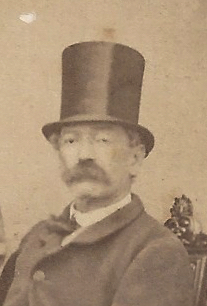
\includegraphics[height=5.5cm]{Fedele} }}%
    \subfloat[Natale Mingazzi]{{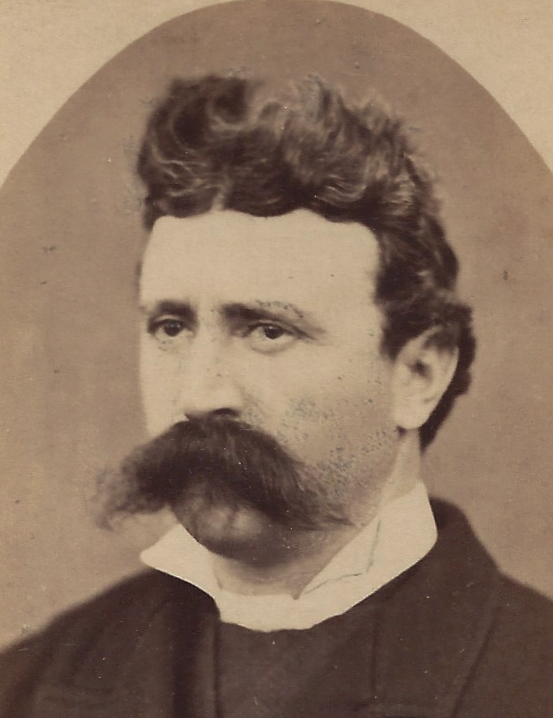
\includegraphics[height=5.5cm]{Natale} }}%
	\vspace{-0.2cm}
\end{figure}

Ho immaginato quindi che Stefano, abbia riportato fedelmente le storie tramandate dal padre e dal nonno, per poi integrare l'opera con le sue storielle.
Inoltre le ultime, benché siano presenti nell'indice, non sono mai state scritte per ovvi motivi. Ho deciso quindi di trascrivere tutte le storielle e di commentarle attingendo informazioni dalle fonti citate nel capitolo \textit{\nameref{fonti} }a pagina \pageref{fonti}.\\

Benché siano storielle palesemente sciocche, presentano parecchi dettagli dell'Alfonsine prebellica e della vita di fine `800 e inizio `900 che sono curiose ed interessanti.




%------------------------------------------------------------------------------
%	CRITERI DI TRASCRIZIONE
%------------------------------------------------------------------------------
\thispagestyle{empty}
\chapter*{Criteri di trascrizione}
La buona calligrafia di Mingazzi ha permesso una facile trascrizione e una discreta comprensione dei concetti che voleva comunicare.\:Tuttavia il testo contiene alcuni errori grammaticali e frasi poco chiare che non permettono la comprensione dell'elemento comico presente in ogni capitolo. Ho scelto quindi di riportare un consistente numero di note a piè di pagina per permettere la comprensione del testo e per arricchire la lettura con curiosità riguardanti i personaggi e i luoghi presentati. Consiglio fortemente di utilizzare queste note per meglio comprendere il testo e per apprendere alcune curiosità sui personaggi e i luoghi presentati. Il testo è stato riportato fedelmente dai manoscritti, ma ho apportato alcune modifiche al fine di una lettura più scorrevole. Per quanto riguarda i titoli dei capitoli ho voluto mantenere quelli dell'indice che si trova all'inizio dei sei quaderni. Siccome in alcuni capitoli vi sono dei sottocapitoli, ho separato questi da titoletti che non erano presenti nel testo originale. L'intero elaborato è stato scritto in \LaTeX\footnote{Scritto anche \LaTeX \: e pronunciato /ˈlatek/ in italiano; errato /ˈlateks/), è un linguaggio di markup usato per la preparazione di testi basato sul programma di composizione tipografica \TeX.} \:dal sottoscritto.\newpage
\noindent Di seguito una foto dell'indice originale:\\
 \begin{figure}[htb]
    \centering
    \vspace{-0.7cm}
    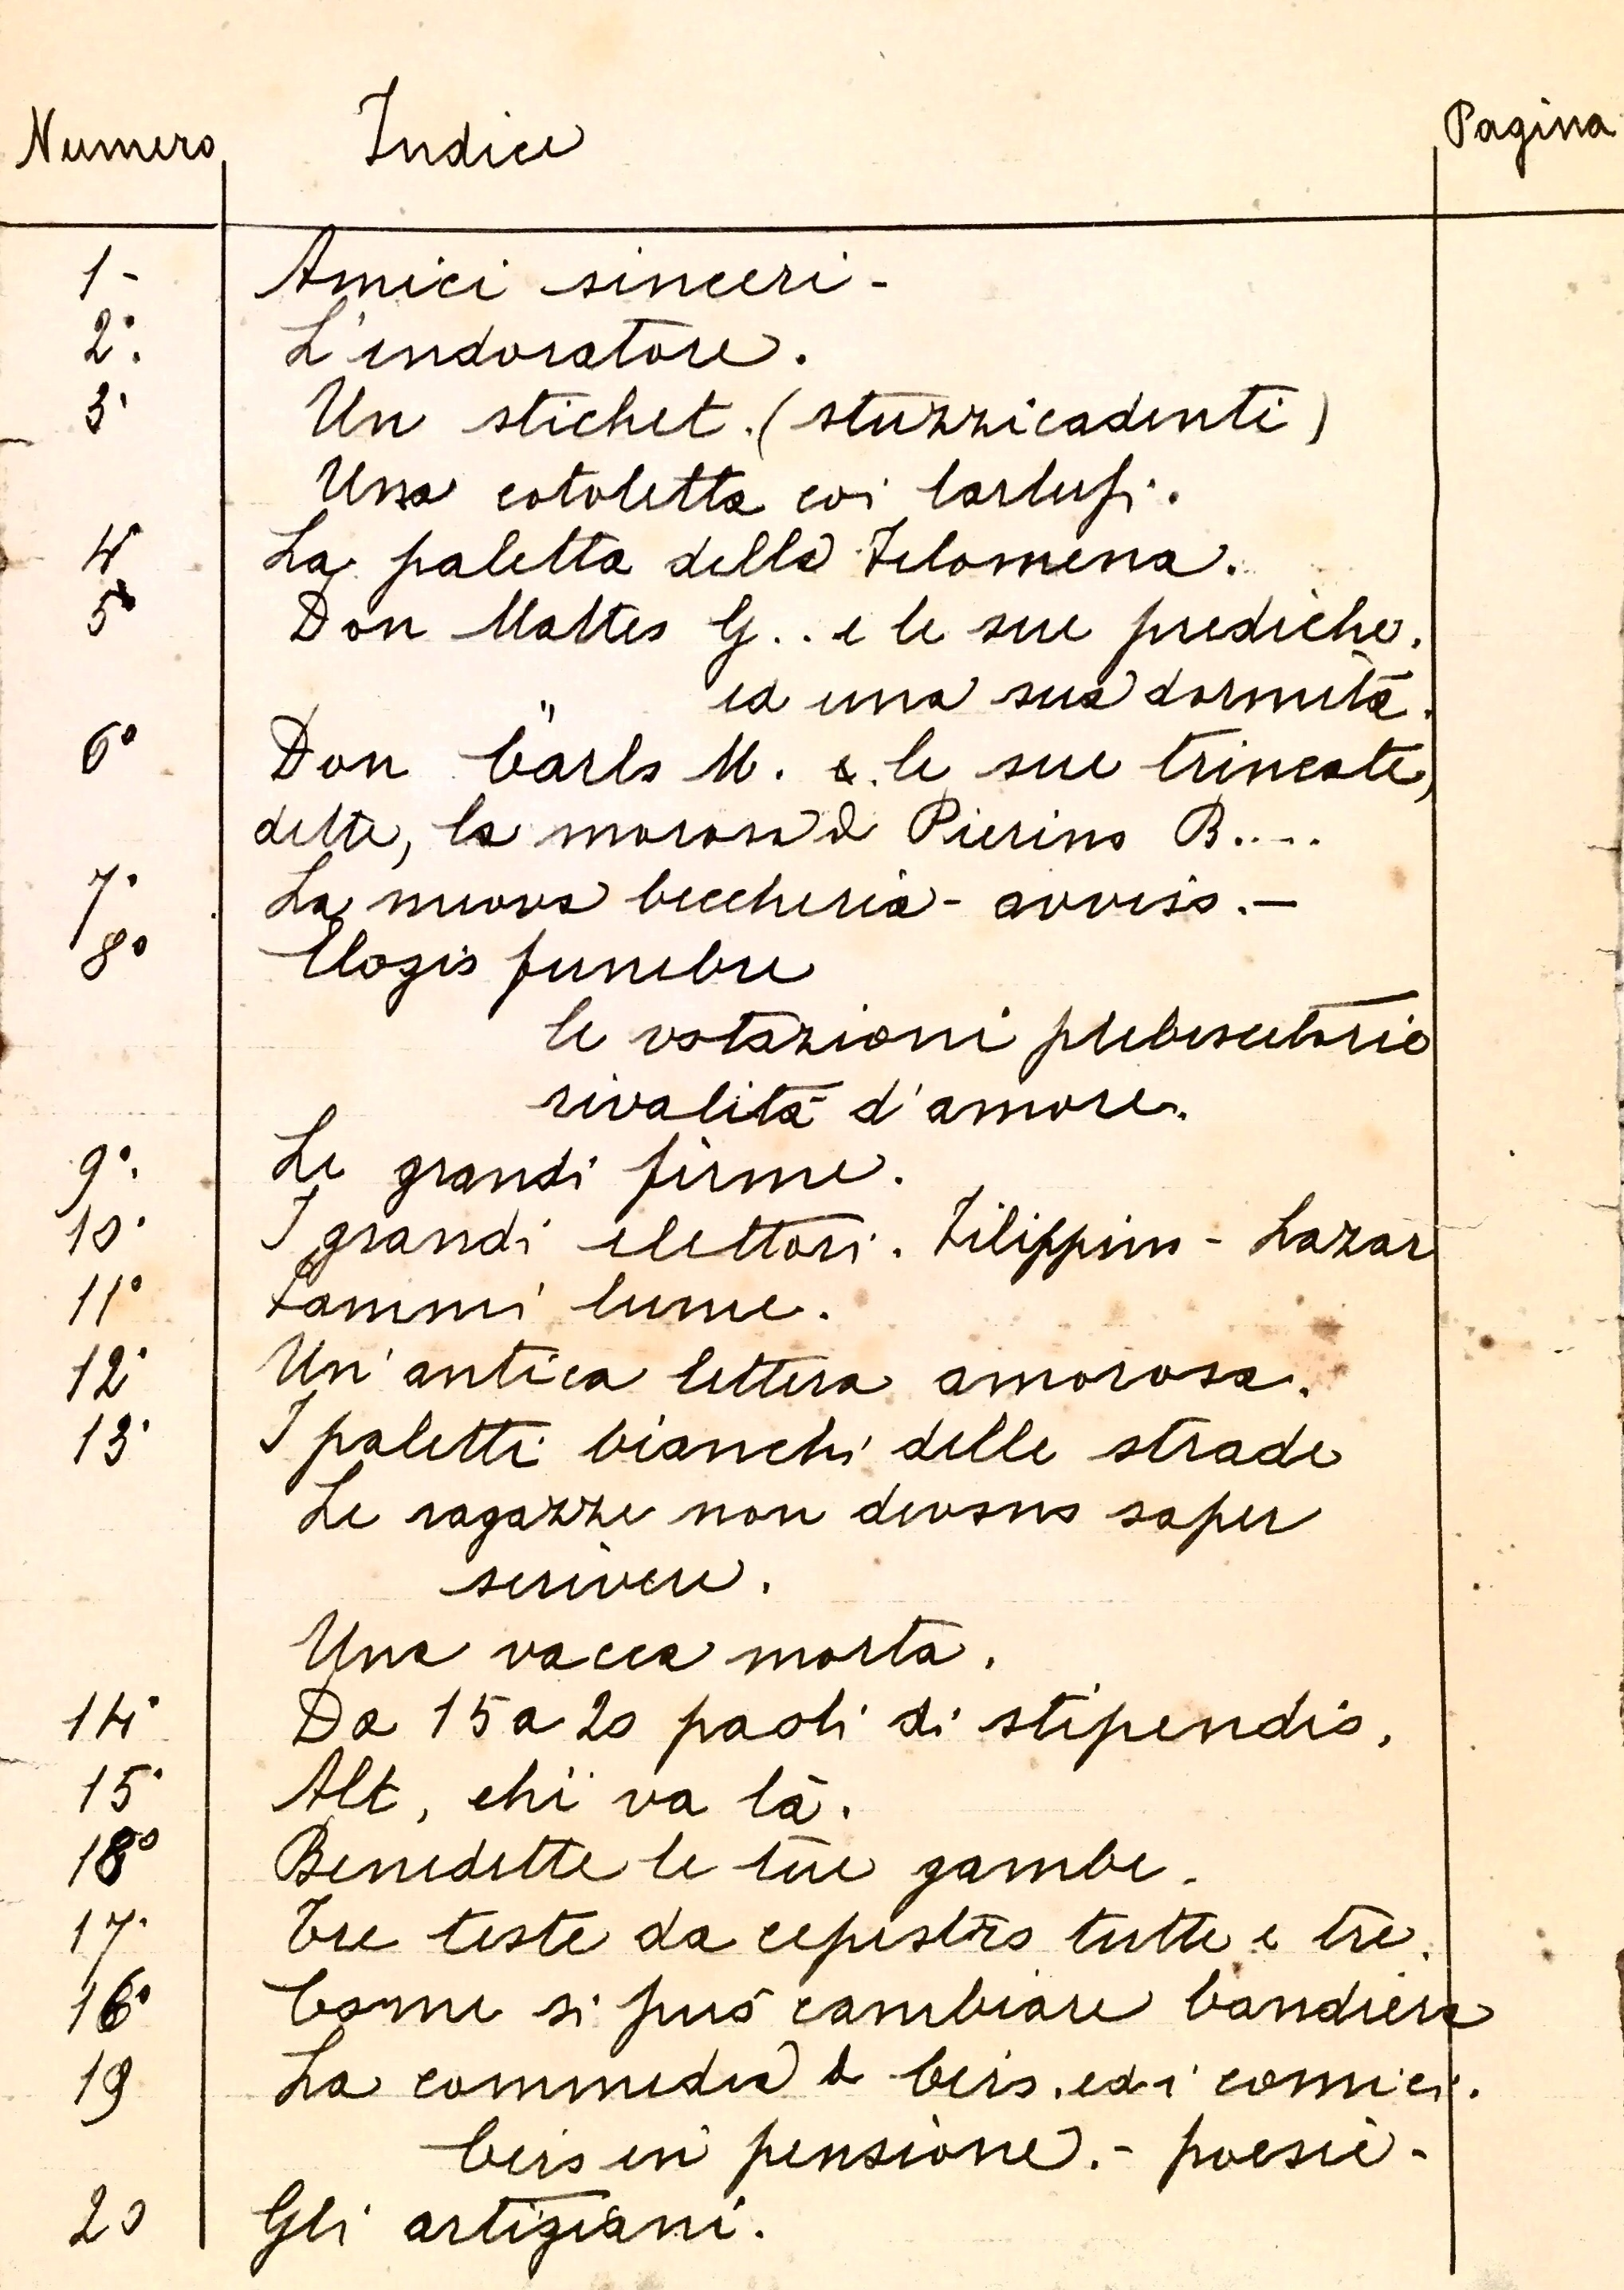
\includegraphics[height=13cm]{indice}
    %\vspace{-0.3cm}t
\end{figure}
\newpage
\noindent Il dialetto scritto da Mingazzi è vistosamente approssimativo: spesso scrive in modi diversi una stessa parola e spesso dimentica accenti necessari per la comprensione. D'altronde è risaputo che il dialetto romagnolo è una lingua relativamente facile da parlare ma di difficile scrittura. Per questo motivo ho aggiunto un minimo di punteggiatura per una buona comprensione, senza però alterare le parole originali, in modo da osservare eventuali diversità tra il dialetto odierno e quello di un tempo. Voglio precisare che molte delle traduzioni in italiano delle frasi in romagnolo, sono state date direttamente da Mingazzi nel testo, tra parentesi. Mi sono limitato a riportare queste traduzioni, tali e quali, nelle note. Per quanto riguarda la punteggiatura, ho scelto di mantenere le virgole nelle posizioni originali, anche se ne risente la comprensione del testo. Una modifica consistente riguarda le citazioni di scritti e di epigrafi che ho riportato al centro della pagina, in corsivo. Per quanto riguarda i dialoghi, ho scelto di munirli di adeguata punteggiatura e di andare a capo quando necessario. Non ho mantenuto lo stesso criterio con cui Mingazzi mandava a capo il testo, ma ho diminuito il numero di questi interventi per motivi di spazio e di leggibilità.	\\\\
\label{fonti}
\noindent A pagina \pageref{Personaggi} ho riportato i personaggi che sono riuscito a riconoscere utilizzando (per ordine di utilizzo):
\begin{itemize}\itemsep2pt
\item{\emph{Storia di Alfonsine}, \index[Personaggi]{Pasi Romano}Romano Pasi}
\item{\emph{alfonsinemonamour.racine.ra.it}, Luciano Lucci\index[Personaggi]{Lucci Luciano}}
\item{\emph{Le Alfonsine, il volto e l'anima}, Giovanni e Maria Francesca Zanzi\index[Personaggi]{Zanzi Giovanni}\index[Personaggi]{Zanzi Mariafrancesca}}
\item{\emph{Quaderni Alfonsinesi}, nella biblioteca Orioli di Alfonsine}
\item{Registri delle Delibere del 1914 e del 1929, nella biblioteca Orioli di Alfonsine}
\item{\emph{I fèt dla veriëla}, Edda Forlivesi\index[Personaggi]{Forlivesi Edda}}
\end{itemize}

A pagina \pageref{Luoghi} ho riportato l'indice di tutti i luoghi presenti nel libro. Per i personaggi e i luoghi più interessanti, ho riportato una descrizione nelle note. Chiedo nuovamente al lettore di prestare attenzione alle note, per meglio comprendere il testo.\\

\vspace{1cm}

Un appello ai lettori esperti: vi prego di contattarmi senza problemi, all'indirizzo email \textit{andraghetti.l@gmail.com} nel caso in cui voleste consigliare qualche correzione o qualche nome mancante.\\

\rightline{Vi ringrazio e vi auguro una buona lettura.}


% Da qui in poi necessito stile bello per i titoli:


%-------------------------------------------------------------------------------
%	CAPITOLO 1
%-------------------------------------------------------------------------------

\chapter{Amici Sinceri}
I reverendi don \index[Personaggi]{Don Salvatori Ruggero}Ruggero Salvatori\footnote{Don Ruggero Salvatori fu un parroco alfonsinese. Oltre ad essere presente nell'indice degli associati all'operetta "Memorie Storiche dell'Alfonsine" di Gian Francesco Rambelli, viene citato al momento dell'assassinio del conte Camillo Foschini per opera di banditi.} e don \index[Personaggi]{Don Faggioli Paolo}Paolo Faggioli erano cresciuti insieme, fatti gli studi ed abbracciato la carriera ecclesiastica. La loro vocazione doveva dunque essere un atto di fede, amor del prossimo e carità cristiana.\\
Bisognava però vivere ed ai piccoli proventi di stola bianca e nera aggiungere qualche altra cosa per il mantenimento decoroso delle famiglie, di relativi fratelli e nipoti, che sempre hanno spolpato i celibi... agiati. Anche in questo pensiero assillante furono d'accordo ed attuarono la speculazione di prendere insieme un podere in affitto di là da Po. Dove precisamente questa unione fraterna trovò le sue discrepanze fu nella divisione degli utili e dei prodotti del fondo\footnote{Il podere, la proprietà che avevano in comune}. \\
Insieme da buoni amiconi, col tradizionale cavallo e biroccino\footnote{Biroccio: carretto porta persone trainato da un cavallo o un asino} si recarono un giorno sul fondo per dividere insieme al colono, il prodotto di un filare di meli. La sorpresa dei due indivisibili amiconi fu grande quando si trovarono a dividere un esiguo mucchietto di mele di scarto... invece della grande quantità conteggiata nella loro mente. Con motto istintivo e temporaneamente i due reverendi inveirono contro il povero colono, tacciandolo di ladro, disonesto... per aver rubato tutte le mele. Agli improperi ed onorifici titoli, seguivano poi le minacce d’escomio\footnote{Cessazione di locazione data a un colono o mezzadro e, anche, la sua esecuzione} da parte dei due reverendi inviperiti... con le faccie accese.\\
Il colono minacciato buttò il dardo... contro le minaccie dei due amici per la pelle e rispose: “don \index[Personaggi]{Don Salvatori Ruggero}Ruggero mi ha ordinato di portargli a casa quattro sacchi di mele, senza che lo sappiate voi don \index[Personaggi]{Don Faggioli Paolo}Paolo. Voi don \index[Personaggi]{Don Faggioli Paolo}Paolo mi avete ordinato di portarvi quattro sacchi di mele. Senza che lo sappia don \index[Personaggi]{Don Salvatori Ruggero}Ruggero. Otto sacchi di mele vi ho portato, altri otto mi sono preso perché dovevano essere di mia parte... e questo è il resto delle mele... da dividere. 
I due reverendi amiconi man mano che il colono parlava e di credere che smettessero il cipiglio fiero e distendessero serenamente le rughe del volto\footnote{La frase è stata riportata fedelmente. Si intende dire che il colono fece capire ai due reverendi che era tutto uno scherzo, provocando una gran risata da parte dei due}... perché entrambi proruppero in una risata...aggiungendo: “Credevo di farvela... invece mi avete prevenuto”.
\begin{center}
\rule{1.5cm}{0.4pt}
\end{center}
Al tempo della vendemmia, ciascuno dei reverendi dispose per portarsi a casa un carro di buon’uva. Il mezzo della gabbatura fu mutato\footnote{Il modo in cui si fregarono a vicenda cambiò}. Due carra di buona uva ed altri due per il colono sul fondo non c’erano. Chi doveva aver la peggio è quel che vedremo. \\
Nei discorsi in sacristia, don \index[Personaggi]{Don Salvatori Ruggero}Ruggero a don \index[Personaggi]{Don Faggioli Paolo}Paolo: “Sentite un po' oggi l’uva è pronta per essere pigiata e portata a casa”.\\
Don \index[Personaggi]{Don Faggioli Paolo}Paolo: “Io, non ci posso però andare, ci mando mio fratello per fare tutto.”\\
Don \index[Personaggi]{Don Salvatori Ruggero}Ruggero: “Va bene, pensate pure voi; io sto a casa a far preparare il tino\footnote{Bacinella per pestare l'uva}”.\\
Verso sera don Ruggero era sugli spini, nell’attesa dell’uva andò sul \index[Luoghi]{Dall'Ara (palazzo)}Crocevia Dall’Ara\footnote{L'incrocio tra via Raspona e via Reale su cui si affaccia il palazzo Dall'Ara ancora oggi esistente, anche se in condizioni pessime. Il palazzo appartenne a Pietro Dall'Ara, reggiano dottore in medicina e chirurgia, stanziatosi in Alfonsine attorno al 1810. Fu eletto Gonfaloniere di Alfonsine nel 1831 e nel 1832 fece costruire un ponte che collegò la strada Reale con la via che portava a Ravenna.} ad aspettare i carri...che non si fecero molto aspettare. Appena apparvero i carri coi contadini don Ruggero li fermo e domandò: “Tu dove devi andare?” - “Da don Paolo” rispose il contadino. “E tu dall’altro carro, dove devi andare?” “Da voi, don Ruggero”. Allora don \index[Personaggi]{Don Salvatori Ruggero}Ruggero, temendo uno scacco, col suo piano in testa tanto ruminato\footnote{Studiato, pensato}, ordinò ai coloni: “Tu, invece di portare il tuo carro d’uva a don Paolo portala a me, e tu che devi venire da me, va da don Paolo” ed ordinato ciò scortò il carro fino a casa sua.\\
Le sorprese vennero alla svinatura del vino. Don \index[Personaggi]{Don Salvatori Ruggero}Ruggero va con la solita confidenza a casa di don \index[Personaggi]{Don Faggioli Paolo}Paolo e gli chiede: “Fatemi sentire il vostro vino nuovo”. Fu subito accontentato, anche perché lo sapevano un ghiottone impenitente. \\
Così si svolse il seguito: don \index[Personaggi]{Don Salvatori Ruggero}Ruggero a don \index[Personaggi]{Don Faggioli Paolo}Paolo “ma com’è buono il vostro vino... mentre il mio è cattivo.” \\
Don Paolo scoppiò a ridere e rispose: “mio fratello ve l’ha fatta perché sapeva che non vi sareste fidato ed avreste disposto sempre il contrario. Ci siete caduto per colpa vostra!”.\\
Don \index[Personaggi]{Don Salvatori Ruggero}Ruggero (mortificato) rispose: “Mi brucia, perché me l’ha fatta un imbecille.”\\
Aveva preso veramente cappello per lo scacco subito\footnote{Si era veramente offeso per il torto subito}, si piantò quindi il tricorno ecclesiastico in testa... e se ne andò a casa di umore più nero della sua veste.\\
L’inganno avrebbe dovuto essergli stato teso da una mente pari alla sua per salvargli la reputazione di furbacchione.\\
%-------------------------------------------------------------------------------
%	CAPITOLO 2
%-------------------------------------------------------------------------------

\chapter{L'indoratore}
Nel \index[Luoghi]{Carraretto Fernè}Carraretto Fernè\footnote{Si intende il quartiere attorno al \textbf{Palazzo Fernè}, ancora oggi presente in via Mameli 3. \index[Personaggi]{Fernè Ferdinando}Ferdinando Fernè era un commerciante di vini all'ingrosso di Bologna ma che aveva un palazzo ad Alfonsine. Maggiori dettagli nell'immagine a fine storiella. (pag. \pageref{fig:villamassaroli})}, allora Massaroli\index[Personaggi]{Massaroli Paolo}, che va ai maceri, vi erano molte vecchie case prima del 1860. \index[Personaggi]{C. Francesco}Francesco C... figlio di buona famiglia nel fiore degli anni e con la blaga del liberalismo contro gli odiati papalini\footnote{Si intende la fissazione del liberalismo. Il liberalismo si ispira a ideali di tolleranza, libertà ed eguaglianza e contesta i privilegi dell'aristocrazia e del clero e l'origine divina del potere del sovrano.}, svelto ardito milite della guardia nazionale, andava a morosa da una tale del \index{Carraretto Fernè}Carraretto. \\
Il suo sentimentalismo aveva parecchie espressioni di adorazione contemplative per la sua bella.
Le scopriva... certe parti, poi battendovi sopra il palmo della mano con carezzevole posa e moine... non si poteva trattenere di esclamare:\\
\indent <<Poverina quanto sei bella, vorrei indorarti\footnote{Ricoprire d'oro}...>>\\
Dillo una sera, dillo due, la cosa andò agli orecchi di certi nottambuli sfaccendati e una sera che il nostro \index[Personaggi]{C. Francesco}Francesco C. era a morosa, sentì bruscamente bussare alla porta, mentre era nella solita contemplazione esilarante.
Si fece buio in faccia; erano i tempi dei ladri e delle bande di Altini\footnote{Altini era un noto brigante che assieme alla sua banda saccheggiava case e sterminava intere famiglie} e di altri e lui temeva... e brusco chiese: <<Chi è?>>\\
Una voce sonora dal di fuori rispose: <<L'indoratore\footnote{L'indoratore era un artigiano che ricopriva oggetti con un sottile strato d'oro}>> e subito a passo di corsa fuggì.
Il nostro buon \index[Personaggi]{C. Francesco}Francesco che aveva tremato alla bussata per la paura di un agguato di ladri, sentendo il nemico che fuggiva si rinfrancò e per la difesa del bel sesso inveì alle stelle: molti ‘boia' di qua, ‘porca' di la, con tutto il coraggio e la forza che può avere chi, deve fare bella figura senza più nulla temere.


 \begin{figure}[htb]
    \centering
    %\vspace{-0.7cm}
    \includegraphics[width=\textwidth]{villamassaroli}
    \caption[Palazzo Fernè - Villa Massaroli]{\textit{Il \textbf{Palazzo Fernè} detto anche \textbf{Villa Massaroli} ancora oggi (2017) presente in via Mameli 3. È attualmente disabitato, e di proprietà degli eredi Pirazzoli. Dalle mappe catastali napoleoniche (e poi gregoriane), risalenti alla prima metà dell'800, il palazzo risulta essere già costruito e di proprietà di \index[Personaggi]{Massaroli Paolo}Massaroli Paolo. I Ferné, proprietari di vaste tenute e di una villa a Lavezzola, si dedicavano soprattutto a produzione e commercio di vino. \index[Personaggi]{Fernè Ferdinando}\textbf{Ferdinando Fernè} sposò nel 1890 una figlia di Massaroli, di nome \index[Personaggi]{Massaroli Diana Anna Cristina `Aunita'}Diana Anna Cristina detta anche Aunita nata nel 1870. Per loro fu arredata la villa che era dei Massaroli e donata come dote alla nuova famiglia. Nel dicembre del 1890 nacque il primo ed unico figlio \index[Personaggi]{Fernè Vincenzo Enzo}Vincenzo Enzo Fernè, che diventerà poi il podestà di Bologna nel 1939. La villa era dotata di uno spazio adibito a cantina per le botti di vino e pare anche di una grande vasca sotterranea dove veniva depositato il vino prodotto e da smerciare a commercianti vari. }}
    \label{fig:villamassaroli}
    %\vspace{-0.3cm}
\end{figure}










































%
%------------------------------------------------------------------------------
%	CAPITOLO 3
%------------------------------------------------------------------------------

\chapter{Un Stichèt}
Il detto \index[Personaggi]{Barèla}Barèla era un macellaio e venditore di carne di pecora. Aveva le sopracciglie folte che gli coprivano gli occhi neri e fondi, i baffi spioventi come due ali d'uccello disarticolate, la faccia rossa e buia, perché sempre poco illuminata dalla scarsa istruzione e mentalità. La grande manifestazione dell'animo suo semplice, che si crede sempre deluso, era la stizza\footnote{Viva irritazione, per lo più momentanea, provocata da un senso di fastidio o di molestia}.\\
\indent Un giorno era andato a Ravenna con chi non gli capitava spesso, e così, fuori del suo ambiente e conoscenze, era impacciato, taciturno e ruminava\footnote{Pensava} molte piccole fantasie nella sua testa, senza sapere con chi sfogarsi. Andò in un'osteria e sentì un tale ordinare una pietanza con un nome nuovo, strano e fuori del suo dizionario. Rimase di stucco quando vide la pietanza: una magnifica bistecca, da fargli venire l'acquolina in bocca e, confacente al suo gusto, per trincare poi un buon bicchiere di quello nero\footnote{Un bicchiere di vino rosso}, credè di evolversi dall'oblicismo\footnote{Voleva evolvere dalla sua ignoranza dicendo al cameriere "un stichèt" credendo di aver ordinato la bistecca} ed ordinò al cameriere <<un stichèt\footnote{Stuzzicadenti}>>. \\
\indent Dopo una lunga attesa ed un lungo assaporamento fantastico richiamò il camerier e gli chiese di portargli <<e stichèt.>>\\
\indent Il cameriere, servizievole disse <<Eccolo, ve l'ho pur portato>> e glielo indicò nel solito piattello sul tavolo.\\
\index[Personaggi]{Barèla}Barèla schizzò veleno, fulminò il cameriere con lo sguardo, trasformato più del solito e di balzo rispose: <<Côssa vut ca megna, di bachèt?>>\footnote{Cosa vuoi che mangi, degli stecchi?}\\
\indent Il cameriere soggiunse: <<Alora côssa vôl?>>\footnote{E allora cosa vuole?}\\
\indent Imbarazzo di \index[Personaggi]{Barèla}Barèla, che richiuse gli occhi, voltò le grandi sopracciglia, la bocca sotto i baffi, si sbiadì, e con voce cavernosa rispose: \\
\indent <<A vòi un quèl còm cl'a magné che sgnór che l'è>>\footnote{Voglio una cosa come quella che ha mangiato quel signore lì} ed alle parole aggiunse l'indicazione fremente con pugno chiuso.\\
\indent Il cameriere: <<Allora deve dire un bistecco!>>\\
\index[Personaggi]{Barèla}Barèla confuso e mortificato, forse temendo di dire un altro strafalcione grugnì: <<Si>> e chinò il mento sul petto per non più fiatare.

Un'altra volta il buon \index[Personaggi]{Barèla}Barèla, che come avrete capito era un semplicione piovuto dal cielo, capitò in un'osteria di Ravenna mentre un suo amico e paesano (un \index[Personaggi]{Fiorentini}Fiorentini) burlone, terminava una cotoletta coi tartufi. All'odore e alla bella vista del prelibato piatto, chiese all'amico quel che mangiasse e quanto costava. L'amico gli rispose che costava due soldi: poi terminò, pagò, se ne andò, mentre \index[Personaggi]{Barèla}Barèla aveva mangiato la prima ed ordinava la seconda, dicendo <<L'è bóna>>\\
Alla seconda, aggiunse la terza e la quarta cotoletta e tirò fuori gli otto baiocchi\footnote{Il termine "baiocchi" può essere inteso come "soldi" in generale. Inoltre 100 baiocchi equivalevano a 1 scudo e dal 1866, 1 scudo era pari a 5,375 lire.} per darli al cameriere.\\
\indent Questi, sorpreso, disse <<Che cosa devo fare?>>\\
\indent \index[Personaggi]{Barèla}Barèla rispose: <<Ma per le cotolette>>\\
\indent E il cameriere: <<Ma costano 8 soldi l'una... quattro per otto trentadue, poi il vino... il pane... >>\\
\indent \index[Personaggi]{Barèla}Barèla frastornato: <<Mo côssa dit? ... an gosta du suld?\footnote{Ma cosa dici? Non costa due soldi?}>>\\
\indent Cameriere: <<No, otto.>>\\
\indent \index[Personaggi]{Barèla}Barèla: <<Vigliac d'un amig quênt cum'à fàt spendar. A putéva magném sol una brasula!\footnote{<<Vigliacco d'un amico, quanto mi ha fatto spendere. Potevo mangiarmi solo una bracciola!>>}>>












































%------------------------------------------------------------------------------
%	CAPITOLO 4
%------------------------------------------------------------------------------

\chapter{La paletta della Filomena}
Nelle nostre vecchie case gli operai non erano stati avvelenati dalla propaganda dell'odio di classe, né imposti in ragione delle loro svogliatezze dai sindacati, ma erano un corpo ed un'anima nella famiglia del datore di lavoro. Beati quei tempi di pace in cui anche i nuovi ricchi non erano ancora venuti a spremere il prossimo ed in ispecie gli operai che dovevansi considerare fidati e parte della loro produzione. In casa del Reverendo Don L. M. i suoi operai trovano sempre una buona mezzella\footnote{Fiaschetto di vino da mezzo litro} di vino (non c'erano ancora i daziari a mettere balzelli\footnote{Imposte} al libero trincare), ed un buon fuoco per cuocere la colazione. La mattina i soliti buoni e bravi operai di casa, preparavano un buon fuoco, una mezzetta di vino e si accingevano alla colazione in cucina, scambiando facezie\footnote{Breve racconto costruito su un motto di spirito} con la serva padrona, la buona \index[Personaggi]{Filomena}Filomena.\\
\indent La confidenza tra la \index[Personaggi]{Filomena}Filomena e gli operai era grande, correvano tra di loro facezie, burle e sarcasmi. Messi in sospetto, gli operai, vollero accertarsi che la \index[Personaggi]{Filomena}Filomena non disertasse di notte il letto di castità della zitellona per altro ancora più casto ed escogitarono una burla atroce che refireremo\footnote{Errore dell'autore: si intende 'riferiremo'} in seguito. \\
Filomena, agli operai radunati a tavola per la colazione, chiese:\\
\indent <<Avete preso la palletta del fuoco?>>\\
\indent E gli operai: <<Chi l'ha vista?>>.\\
\indent E così per otto giorni di seguito durò il dialogo al quale però interrogante e gli interrogati sembrava non dessero importanza alcuna. Al nono giorno la domanda ripetuta dalla \index[Personaggi]{Filomena}Filomena si oscurò e comincio ad inalberarsi ... da serva padrona, ma uno degli operai, il più vecchio, con cipiglio ironico mise le cose a punto dicendo:\\
\indent <<La paletta è nel tuo letto e se tu fossi andata a dormire nel tuo letto l'avresti trovata. Invece sei andata a dormire col prete... e noi abbiamo voluto provartelo.>>\\
Come rimasero per questa trovata, la \index[Personaggi]{Filomena}Filomena ed il prete è facile immaginarlo. Il fatto ancora fa ridere i vecchi del paese.

\vspace{0.2cm}
\centerline{\rule{1.5cm}{0.4pt}}
\vspace{0.2cm}

 \begin{figure}[htb]
    \centering
    %\vspace{-0.7cm}
    \includegraphics[width=\textwidth]{mingazzigente}
    \caption[Mingazzi con altri (1925)]{\index[Personaggi]{Mingazzi Stefano}Mingazzi a destra e in basso la governante `Ghina' con il cane pastore maremmano di Stefano, `Negar'. A sinistra si riconosce un giovane \index[Personaggi]{Zoli Cesare}Cesare Zoli. Le tre persone al centro non sono state riconosciute. La foto dovrebbe essere stata scattata negli anni '20 quando Mingazzi non era ancora sposato.\index[Personaggi]{Mingazzi Stefano}\label{fig:mingazzigente}}
    %\vspace{-0.3cm}
\end{figure}
%------------------------------------------------------------------------------
%	CAPITOLO 5
%------------------------------------------------------------------------------

\chapter{Don Matteo G. e le sue prediche}
\index[Personaggi]{Don G. Matteo}Era un buon diavolo, senza istruzione, sacerdote di Cristo e... di Bacco, unico suo peccato.\\
\indent Fino alle 20,45 stava chiuso nella sua cantina a trincare di quel buon vino ... al quale aggiungeva dell'alcool, perché era troppo debole. Dalle 20,45 diventava astemio per preparasi col digiuno alla Santa Messa del mattino successivo. Non è da tacere che andava sempre a letto in garletta\footnote{Essere "in garlèta" di solito si dice di persona allegra, un po' sopra le righe, magari per qualche bicchiere di vino in più.} orando per forza d'abitudine. Celebrava continuamente la messa a San Francesco ed a Sant'Apollonia\footnote{AGGIUNGERE SAMARITANI VINCENZO San Vincenzo viene anche chiamata Santa Apollonia per il quadro dell'omonima santa che vi è all'interno. S. Vincenzo fu fabbricata circa il 1750 da Francesco de' conti Cervi Samaritani, famiglia venuta da Cremona nel 1509. Diventò un oratorio padronale di proprietà di Stefano Mingazzi. Oggi è di proprietà dei Minguzzi.} al \index[Luoghi]{Passetto}Passetto. Le popolazioni delle due strade gli volevano molto bene, ricorrevano a lui per gli annunzi dall'altare e subito lui li accontentava coi i seguenti pistolotti\footnote{Discorso ammonitorio ed esortativo} autentici:\\
\indent <<Popolo della \index[Luoghi]{Reale (via)}via Reale, è stato perduto un bottazzo\footnote{Direttamente spiegato dal Mingazzi nei suoi quaderni: "Per chi non lo sapesse, il bottazzo era un fustico, piccolo barile, di legno che i contadini portavano nel prato, in valle, col vino da bere durante i lavori"} pieno di vino; chi l'avesse ritrovato si beva il bottazzo e porti il vino...>> poi <<No, no am so sbaglié\footnote{<<No, no mi sono sbagliato>>} voglio dire si beva il vino e porti il bottazzo.>>\\
\indent Altro esempio:\\
\indent<<Popolo della \index[Luoghi]{Reale (via)}via Reale, è stata perduta una gabana\footnote{Termine dialettale per 'giacca'} color di mezzalana\footnote{Don Matteo sbaglia l'associazione colore-materiale}, chi l'avesse ritrovata la porti...>>

I pistolotti suoi personali erano ancora più curiosi. \index[Personaggi]{Magrini}Magrini e altri ragazzi, gli disturbavano la messa, allora il buon prete semplicione, tralasciava le funzioni, si infiammava , e poi:\\
\indent <<Sa vègn fùra cun sta vinciastra a va més mè.\footnote{<<Se vengo fuori con questo vimine vi accomodo io>>}>>\\
\indent Le cose si quietavano per un po' poi i monelli ricominciavano ed il povero don Matteo\index[Personaggi]{Don G. Matteo} abbandonava la messa, pigliava il vimine e vestito dei sacri paramenti rincorreva i monelli per il cortile per picchiarli... I fedeli ridevano e compativano. \\
La fine della sua officiatura\footnote{Celebrazione della funzione religiosa} a \index[Luoghi]{San Vincenzo}S. Vincenzo fu proclamata da lui dall'altare, così:\\
\indent <<Popolo della via Reale\index[Luoghi]{Reale (via)} la Sgnora \index[Personaggi]{Lanconelli Filippina}Flipèna, l'è môrta, \index[Personaggi]{Samaritani Vincenzo}Samartèn (allora padrone dell'oratorio) un'um pêga, e mè, la messa par gnint an la vèngn pui a dì\footnote{<<La Signora Filippina è morta, e Samaritani non mi paga, e io, la messa per niente non la vengo poi a dire>>}>>\\
Con questa chiusa\footnote{Conclusione} cominciò la sua nuova officiatura al \index[Luoghi]{Passetto}Passetto. Colà i contadini andavano a messa con lo schioppo\footnote{Fucile}, del quale il nostro don Matteo\index[Personaggi]{Don G. Matteo} aveva un sacrosanto terrore. Allora uscì in uno dei suoi predicozzi:\\
\indent <<Popolo del \index[Luoghi]{Passetto}Passetto, vi proibisco di venire alla santa messa c'un che cazz che sbat, pet a cl'êtar, uv putrèb scapé una sciupté e amazé e povar zazardòt a l'altér cl'è inuzènt\footnote{<<...con quel cazzo che batte dirimpetto a quell'altro, vi potrebbe scappare una fucilata ad ammazzare il povero sacerdote, all'altare, che è innocente.>>}>>\\

Chiudiamo con un'ultima del semplicione. Funzionava da cappellano a \index[Luoghi]{Savarna}Savarna ed un giorno, verso sera, montato sul suo birroccino tirato dall'asino si prese da Alfonsine per tornare in parrocchia. Come il solito, aveva sul pomeriggio troppo brindato a Bacco e mal si reggeva in gambe. Nei pressi della \index[Luoghi]{Le Marianne}Scoperta delle Marianne, sentì la necessità di una occorrenza... piantò l'asino della strada e si appiattì al di là di una siepe.

Quel che successe si deve indovinare; l'asino fu trovato alla mattina, coi finimenti, attaccato al biroccino, dietro la porte della stalla della Chiesa a \index[Luoghi]{Savarna}Savarna, ma del padrone nulla.

A mattino molto inoltrato, il prete si svegliò nel prato, dove era caduto per la solenne sbornia, perché il sole lo martellava... riandò agli avvenimenti della sera prima e nella mente un po' rischiarata, non trovando più l'asino... lo seguì a piedi... da buon soldato di Cristo.














































%


%---------------------------------------------------------------------------
%	CAPITOLO 6
%---------------------------------------------------------------------------

\chapter{Don Carlo M, le sue trincate e la morosa di Pierino Bonafirma}
\index[Personaggi]{Bonafirma Pierino}
\index[Personaggi]{Don G. Matteo}Don Matteo aveva non solo dei colleghi, ma anche degli imitatori. \index[Personaggi]{Don M. Carlo}Don Carlo M. cappellano della nostra parrocchia, era una macchietta\footnote{Un personaggio molto originale} molto originale. La mattina si alzava presto, per adempiere alle funzione della Santa Messa poi immediatamente si spogliava dei sacri paramenti, si calcava il tricorno a sbilenco in testa, pigliava il bastone e via attraverso la piazza entrava nel bettolino\footnote{Spaccio di vini e pietanze} ed ordinava una paglietta di acquavite\footnote{Fiaschetto di acquavite ricoperto esternamente di paglia} grossa (circa 1/8 di litro) poi alla prima vi aggiungeva molte altre fino alle 8-9 e dopo andava a casa per prepararsi il desinare\footnote{Consumare il pasto principale della giornata, pranzare}. Appena mangiato schiacciava un pisolino, poi attaccava il cavallo ad un birocino color turchino, col sedile fermo su due grosse cinghie, che servivano da molle, e imprimevano a chi si sedeva il movimento del cavallo. Stava seduto in mezzo al cuscino di traverso, col tricorno sulle ventitré da sembrare un aquilone che prende quota; rosso in faccia con due occhi bianchi, sembrava la reclame\footnote{Pubblicità, propaganda commerciale} della canina\footnote{Canina, vino romagnolo da tavola. (da distinguere dalla Cagnina, vino dolce romagnolo)}.

Tutto il giorno era affaccendato per dare benedizioni e maledizioni ai topi, ai grilli, alle rughe, alle talpe ecc. Il volgo aveva una ferma convinzione che le maledizioni di don Carlo\index[Personaggi]{Don M. Carlo}, se ben calcate da lui, erano un portento per il buon esito delle loro speranze. Parlava a scatti, con voce nasale ed appena discendeva per le sue funzioni nel cortile di un contadino, chiedeva del buon vino. Il vino, quello buono, era tenuto gelosamente dai contadini nelle botti ben colme e non a mano\footnote{Non nelle bottiglie, né in fiaschi}. Allora si svolgeva questo dialogo. \\
\indent Don Carlo\index[Personaggi]{Don M. Carlo}: <<Et la tromba\footnote{<<Hai la tromba?>> - Arnese per aspirare il vino da una damigiana o da una botte.}?"\\
\indent Contadino: <<No Sgnor\footnote{No signore}>>.\\
\indent Don Carlo\index[Personaggi]{Don M. Carlo}: <<Alora a jò e sòrg mè\footnote{<<Allora ho il sorcio io>>}>> e tirava fuori un grosso arnese di latta da contenere vari litri... che erano in breve trincati\footnote{I litri di vino vennero bevuti in breve tempo dal prete}.\\

Era caratteristico anche nelle funzioni della messa; bisognerebbe però aver sentito la sua voce, nasale a scatti, nervosa e nasale per meglio gustare il tipo. Appena il chierico vuotava l'acqua nel calice, diceva: <<Basta, basta...>>. Quando smetteva di vuotare\footnote{Versare} il vino, <<vuta... vuta... vuta dóca>>\footnote{<<Versa, versa, versa dunque>>} e non era contento finché il prelibato vin santo non era sgocciolato interamente dalla sacra ampollina nel calice.\\
\index[Personaggi]{Samaritani Vittorio}V. Samaritani era proprietario dell'oratorio di \index[Luoghi]{San Vincenzo `Sant'Appollonia'}San Vincenzo che più non faceva officiare e trascurava.\\
Un giorno passando il nostro prete dalla via ... trova Samaritani sulla strada, ferma il ronzino, e gli rivolge il discorso testuale:\\
\indent <<Ui, al tratè molt mel che casant\footnote{<<Ei, lo trattate molto male quel casante>>}>> ed indicava con la frusta l'oratorio.\\
\indent V. rise, come per scusarsi.\\
\indent Don Carlo\index[Personaggi]{Don M. Carlo} allora: <<T'niv in t'la ment cun an dega cumbien e vostar casant>>\footnote{Letteralmente; <<Tenetevi in mente che il vostro casante non vi dia commiato>>. Come per dire: <<... deve sperare che il vostro edificio non vi dia lo sfratto>>} poi frustò il cavallo e via col solito tric-trac.\\

Esercitava la confessione, in maniera curiosa. Un giorno gli si presenta alla grata del confessionale una bella figliola. Ed eccone il referto genuino:\\
\indent \index[Personaggi]{Don M. Carlo}Don Carlo: <<Fasiv l'amor\footnote{<<Fate l'amore?>>}?>>\\
\indent Ragazza: <<Si>>\\
\indent \index[Personaggi]{Don M. Carlo}Don Carlo, arricciando il naso e con una smorfia: <<een>> (che sembrava un grugnito).\\
\indent Poi: <<Cun chi\footnote{<<Con Chi?>>}?>>\\
\indent Ragazza: <<Con \index[Personaggi]{Bonafirma Pierino}Pierino d'Bonafirma>>\\
\indent \index[Personaggi]{Don M. Carlo}Don Carlo: <<Bonafirma... E pu cossa fasiv\footnote{<<E poi cosa fate?>>}?>>\\
\indent Ragazza: <<Sol... in tal m...\footnote{Mingazzi ha volutamente coperto le parole con i puntini: <<Solo... nelle m...}>>\\
\indent \index[Personaggi]{Don M. Carlo}Don Carlo: <<Spudurè... E vostra medar?\footnote{<<Spudorato... e vostra madre?>>}>>\\
\indent Ragazza: <<La s'indurmêta\footnote{Si addormenta}>>\\
\indent \index[Personaggi]{Don M. Carlo}Don Carlo: <<Ruffiana>> e non fu una voce, ma un ruggito.\\


\newpage

 \begin{figure}[htb]
    \centering
    %\vspace{-0.7cm}
    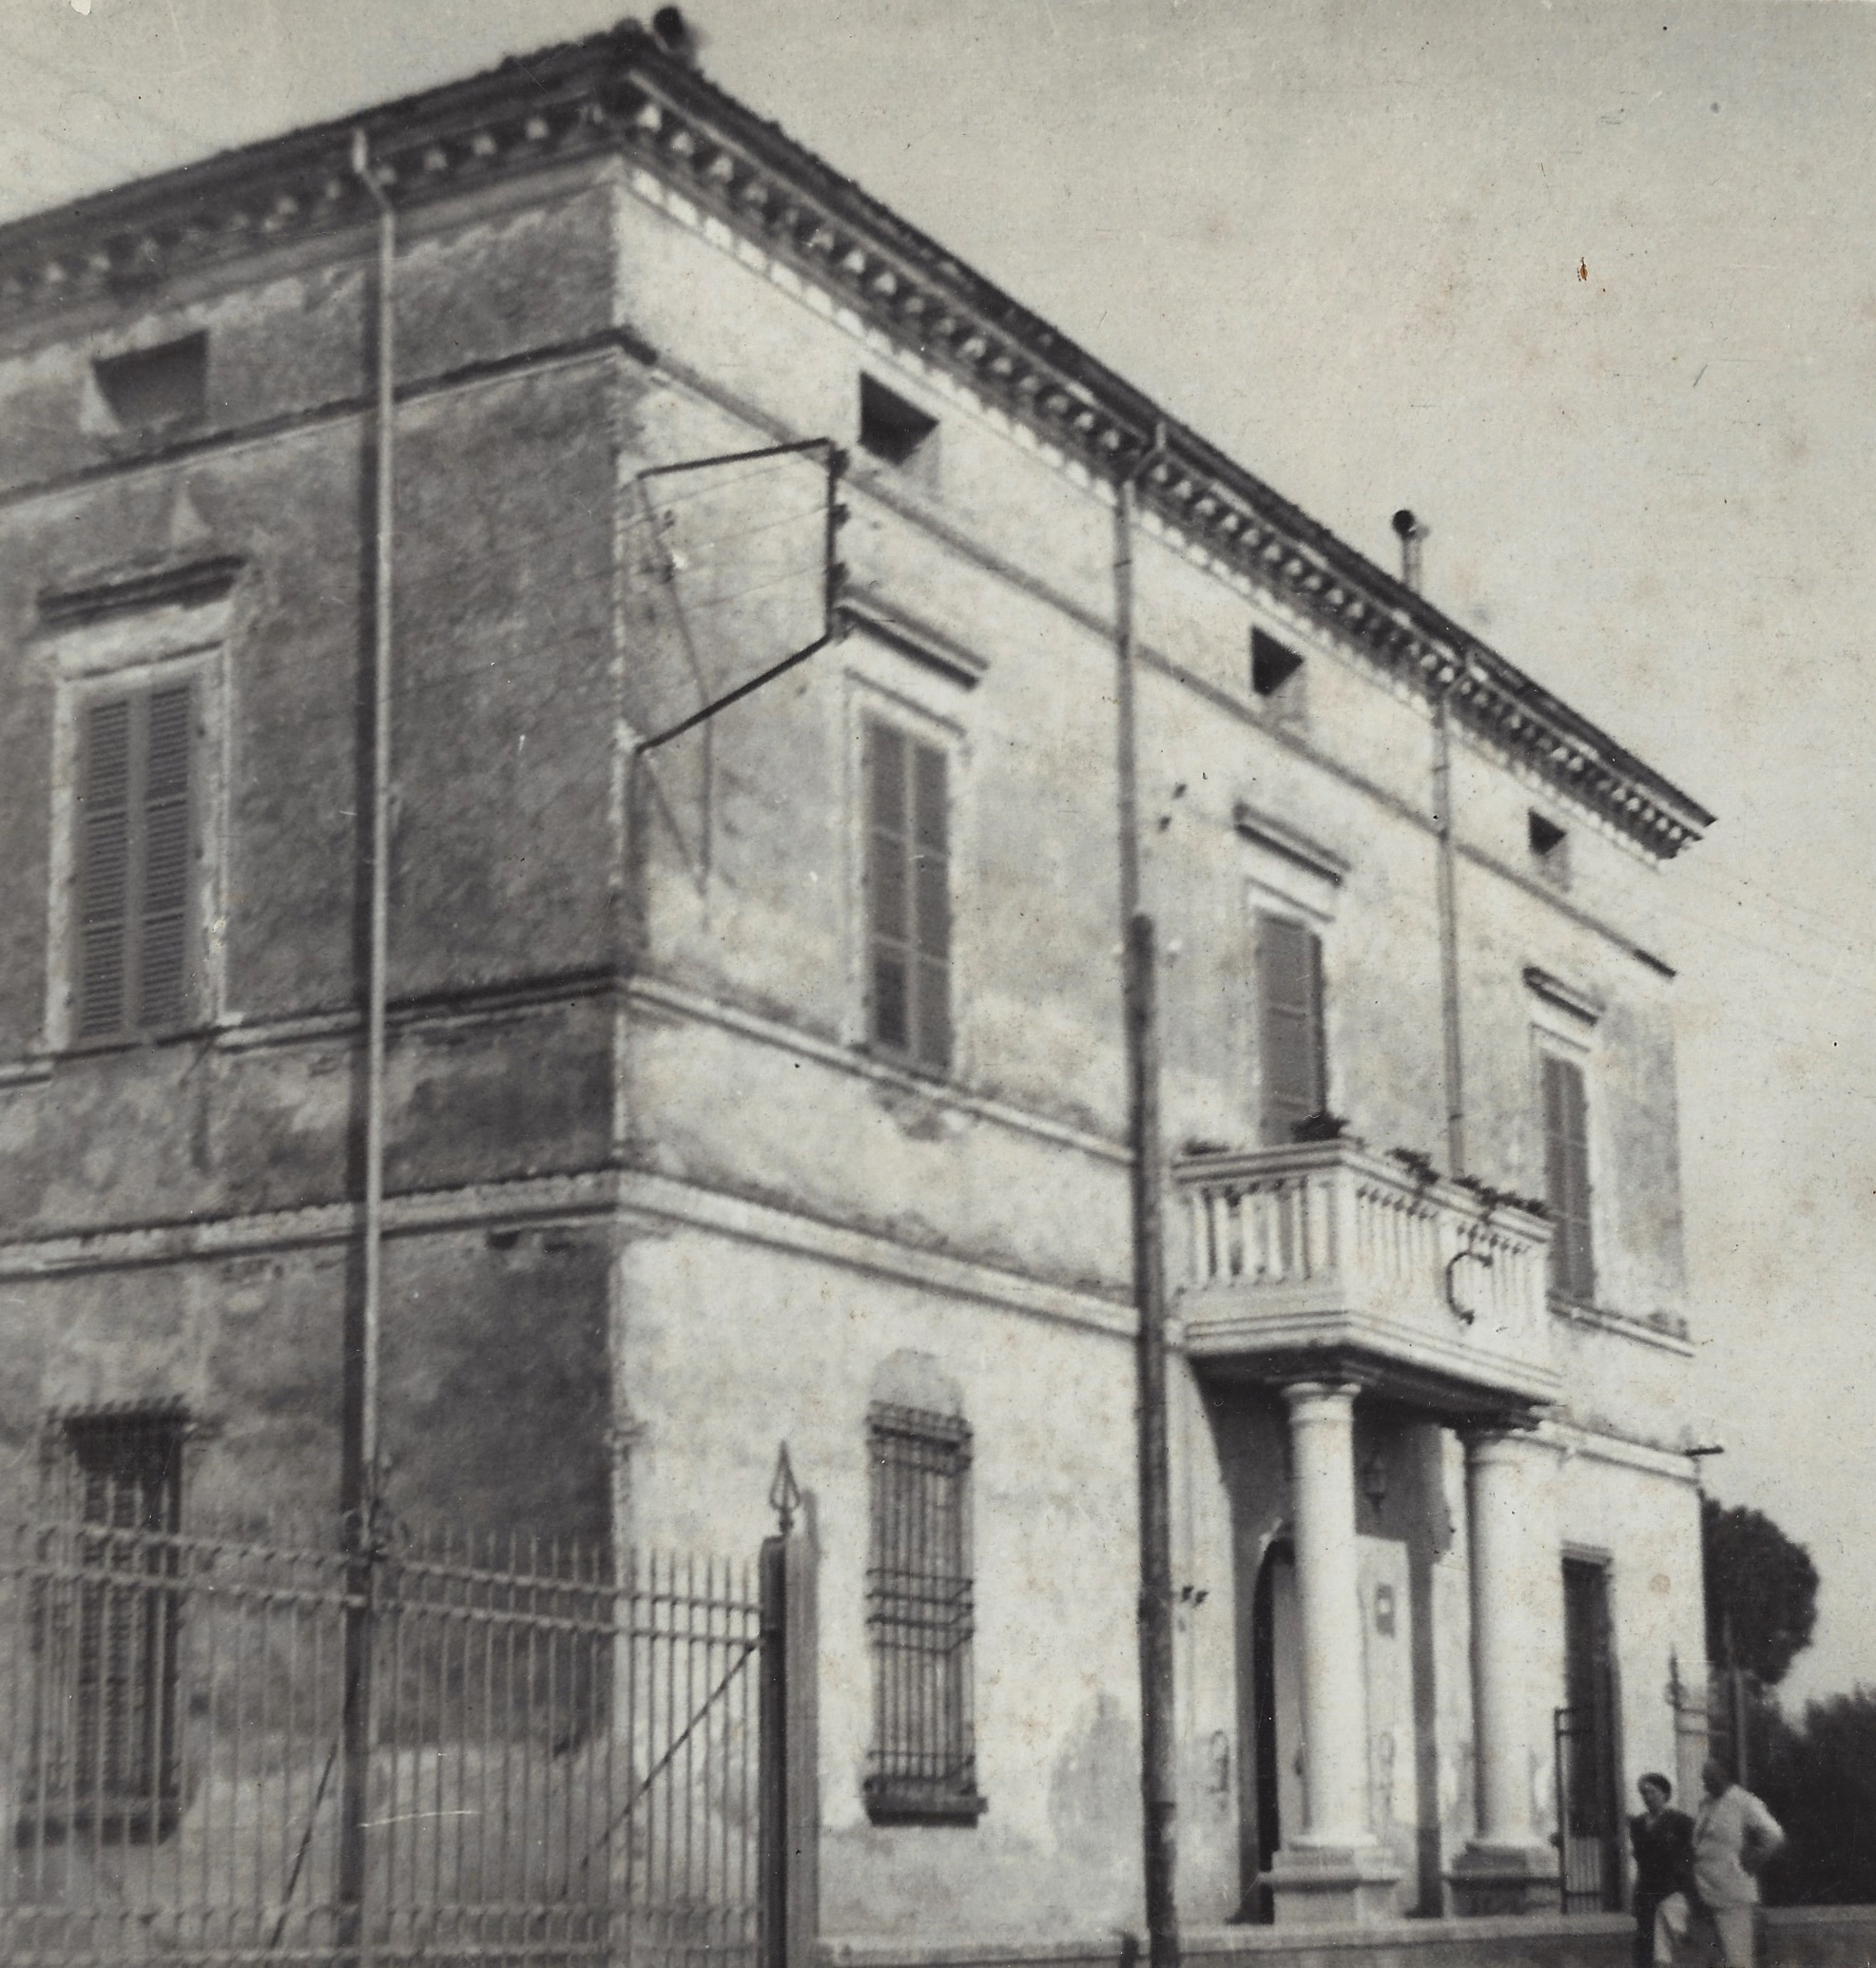
\includegraphics[width=\textwidth]{casamingazzi}
    \caption*{Il \textbf{Palazzo Mingazzi}, in via Reale 97. In basso a destra si può notare Stefano Mingazzi con la moglie Amalia Isani. Alla morte di Amalia, la casa passò all'erede universale di Mingazzi, ovvero l'Istituto dei Ciechi di Bologna. Minguzzi Egisto comprò tutti i terreni tra cui anche il palazzo Mingazzi. Questo edificio non era in buone oncdizioni perciò Egisto decise di abbatterlo. (ndr) Dalle testimonianze che ho raccolto, all'entrata si poteva vedere subito una ripida ma maestosa scalinata in legno.\label{fig:casamingazzi}}
    %\vspace{-0.3cm}
\end{figure}



































%
%------------------------------------------------------------------------------
%	CAPITOLO 7
%------------------------------------------------------------------------------

\chapter{La Nuova Beccheria - Avviso}
\index[Personaggi]{Gioele}Gioele\footnote{\textbf{Gioele}, (ndr) quelli che l'hanno conosciuto, mi hanno raccontato che Gioele, o Giuele, stava seduto davanti ad un caffè dove dava dei pareri. Veniva pagato in natura, quindi con un salame o cose del genere.} calzolaio che aveva disertato da un pezzo il dischetto\footnote{Il dischetto era il tavolino usato dai calzolai nel loro lavoro} per vivere con le bricciole della rendita degli altri: pur di non fare nulla, si peccava di essere un superuomo, un grande elettore, causidico\footnote{Chi difendeva qualcuno in giudizio senza essere avvocato}, letterato. Di tutta l'arca della sua scienza aveva solo la miseria del letterato. S'intrufava\footnote{Intrufolava} ed era un assiduo degli spettacoli pubblici, come le prove dei cavalli sullo stradone, le cause in pretura, le adunanze\footnote{Riunioni comunali} al consiglio comunale, le baruffe in piazza, il montaggio e lo smontaggio dei baracconi dei saltimbanchi e cose di quanto può occorrere a chi non ha né arte né parte ad uno sfaccendato per ingannare il tempo ed emergere\footnote{[...]e tutto ciò che può servire ad uno sfaccendato, che non ha nessun lavoro, per passare il tempo.}.\\
\indent Un giorno gli si presenta \index[Personaggi]{Ettore Pagani, Gena (macellaio)}Ettore Pagani\footnote{\textbf{Ettore Pagani}, la memoria storica vuole che ad Alfonsine vi sia sempre stata una macelleria di "Gena", appunto Pagani.} e lo prega di fargli un avviso al pubblico perché vuole aprire una nuova beccheria. \\
\indent Il nostro \index[Personaggi]{Gioele}Gioele trionfante, per l'onore e col miraggio forse del guadagno di una bracciola, si prende \index[Personaggi]{Ettore Pagani, Gena (macellaio)}Pagani e lo porta in farmacia, dove era di casa un po', e dove trovava gratis, carta, penna e calamaio e persone che l'attorniavano per ridere alle sue spalle.\\
\\
\indent Ecco l'Avviso:

\textcal{ \Huge
\vspace{-1cm}
\begin{center}
	Avviso
\end{center}
\begin{center}
	Nella bottega di \index[Personaggi]{Faccani Rodolfo (commerciante)}Faccani Rodolfo barbiere viene aperta una bottega di carne da bue.\\
\end{center}
\begin{center}
	d'avanti L 1 al Kg\\
	didietro L 1.20 al Kg
		\rightline{Pagani Ettore}
\end{center}
} \normalsize \normalfont 

\indent Letto forte a chiara voce, provocò risata.\\\\
\index[Personaggi]{Vincenzo della Borghina} Vincenzo della Borghina s'azzardò di dire: <<la carne di bue... è al fieno \footnote{(ndr) Dopo varie letture ed interpretazioni, non sono riuscito a trovare un senso a questa frase. Forse intendeva dire che la carne al fieno era pregiata e dire "didietro" la screditava.}>>\\
\indent\index[Personaggi]{Gioele}Gioele: <<Dam a qua e manifest. E poi imbezèl a vut ca dèga `carne da cul'?\footnote{<<Dammi qua il manifesto. E poi, imbecille, vuoi che dica `carne da culo'?}>>. \\
\indent Aspetta.\\
\indent Prese il manifesto corresse borbottando <<Sumàr a vit ac azonz `ora'\footnote{<<Somaro, vedi, aggiungo `ora'>>}>>
\newpage
\textcal{ \Huge
\begin{center}
	Avviso
\end{center}
\begin{center}
	Nella bottega di \index[Personaggi]{Faccani Rodolfo (commerciante)}Faccani Rodolfo barbiere viene aperta \underline{ora} una bottega di carne da bue.\\
\end{center}
\begin{center}
	d'avanti L 1 al Kg\\
	didietro L 1.20 al Kg\\
	\rightline{Pagani Ettore}
\end{center}
} \normalsize \normalfont
<<A vit ora cum ca deg. Portal a la stêpa e pu dì cu la fat Giuèla!\footnote{<<Vedi ora come dico. Portalo alla stampa e dì che l'ha fatto Gioele.>>}>>\\
\indent E così fu stampato e consacrato alle risate del pubblico.















































%

%-------------------------------------------------------------------------------
%	CAPITOLO 8
%-------------------------------------------------------------------------------

\chapter{Elogio Funebre - Le votazioni plebiscitarie - Rivalità d'amore}
\subsection{Elogio Funebre}
Il signor C. B. era uno stimato e ricco negoziante. Si deve anche dire che impersonava anche un po' troppo del suo ‘io' e dopo non vedeva altro, coi suoi interessi.\\
Rimasto vedovo, senza troppa commozione seppe tessere il seguente elogio funebre in lode della sua metà:
"Va, o mia Antonia, quando venisti in casa mia, mi portasti mille scudi ed ora con venticinque paoli\footnote{1 scudo = 10 paoli = 100 baiocchi} ti mando al cimitero."\\
\subsection{Le votazioni plebiscitarie}
Come partito politico tendeva al papalino, e non voleva sentire troppo parlare di liberali, che gli disturbavano il negozio. Tuttavia sapeva stare molto tra color che son sospesi\footnote{Sapeva stare con persone che non avevano rilevanti tendenze politiche} e non si sbilanciava molto, anche perché le sue idee erano in minoranza coi suoi accoliti.\\
Era solito andare nel ferrarese col biroccio per vendere molte botti d'acquavite. In occasione del plebiscito del 1860\footnote{Il 21 ottobre del 1860 si svolse il plebiscito per l’annessione del Regno delle Due Sicilie al Regno di Sardegna. Quel giorno il 79\% degli aventi diritto al voto si espressero per il Sì.} i conti Fuschini, accesi liberali, seppero che il Signor C. B. era tornato allora dal ferrarese ed ansiosi di notizie gli mandarono un biglietto concepito:\\
"Diteci come sono andate le votazioni nel ferrarese."\\
Il Signor C. non volle sbilanciarsi e rispose:\\
"Quando vado sul ferrarese mi occupo di vuotare le mie botti, altro non so di votazioni."\\
La spiritosa risposta provocò risate e rimase celebre. \\
\subsection{Rivalità d'amore}
Per amore e profondità nel dolce parlare Italiano il nostro Signor C. è anche rimasto celebre. Si era innamorato di una bella ragazza, lui attempato e con due baffoni spioventi come due nere saracche\footnote{La salacca, saraca o sarachina è la definizione commerciale di alcuni tipi di pesce}. \\
Il male venne, che la sua bella aveva un'altro adoratore in un giovincello sbarbato, uno sbarbatello, come si direbbe.\\
Geloso, irato contro lo sbarbatello il nostro Signor C. innanzi allo specchio, pavoneggiava la sua carattestica di fiero uomo, contro il disprezzato sbarbatello e provava le mosse da fargli per avvilirlo e le parole da dirgli; avvicinandosi allo specchio con enfasi:\\
Si tirava su i mustacchi\footnote{Baffi} ricciandoli, poi sghignazzante: "... e di questi voi non ne abbiate."\\
Secondo il suo ‘io' lui era un uomo il rivale invece un fanciullo a balia.



%--------------------------------------------------------------------------
%	CAPITOLO 9
%---------------------------------------------------------------------------

\chapter{Le grandi firme}
Le nostre amministrazioni hanno avuto il privilegio di essere mandate alla storia per le grandi firme che le hanno assunte.\\
Infatti leggiamo\footnote{Anticipo ai lettori che le firme sopracitate, sono appartenenti ai personaggi di alto rango che sbagliavano a scrivere il proprio nome, o lo facevano in modo incomprensibile. Mingazzi ha riportato le firme erronee degli assessori Fagioli Angelo, Natali Alessandro e dei consiglieri comunali Poletti Raffaele e Garavini Battista}\footnote{\textbf{Natali Alessandro}, un assessore supplente nella giunta comunale del 1902, con \index[Personaggi]{Alberani Alberto}Alberani Alberto indaco}:
\textcal {\\\\
\Huge
	\centerline{ \:L'assessore \: \: \: \: \: \: L'assessore}\\
	\centerline{Angolo Fagolo  \: \: N. Alessandro}\\\\
	\centerline{Il membro della Cong. Carità}\\
	\centerline{G. Severo}\\
}\\ \index[Personaggi]{Angelo Fagioli (assessore)} \index[Personaggi]{Natali Alessandro (assessore)} \index[Personaggi]{G. Severo}
\normalfont
\footnote{Congregazione di carità è la denominazione ottocentesca delle istituzioni statali destinate a venir incontro ai bisogni della popolazione povera. Era legata all'\index[Luoghi]{Ospedale G. Gamberini di Alfonsine}Ospedale G. Gamberini di Alfonsine e ne gestiva le donazioni.}\\
\indent Vi erano poi anche ai margini delle amministrazioni altre firme di valore:
\textcal {\\\\
\Huge
	\centerline{\index[Personaggi]{Poletti Raffaele (consigliere comunale)}Paffaele Roletti}
}\\ \\
\normalfont
firma che valeva molto su di una cambiale\footnote{Nel diritto italiano, è un titolo di credito la cui funzione tipica è quella di rimandare il pagamento di una somma in denaro.} anche perché l'artefice prima di stamparla aveva bisogno di provare molte paia di occhiali, poi accusava di non trovarne un paio adatti, poi la penna si spuntava, la carta si forava, l'inchiostro macchiava, non scorreva, mezz'ora prendeva la posizione adatta, e racconti della caduta del papa tra una sillaba e l'altra, quella della cacciata dei carabinieri del papa ecc. ecc. e finalmente dalle 9 alle 12 poteva uscire la gran firma. \\

\indent Altra firma era
\textcal {\\\\
\Huge
	\centerline{\index[Personaggi]{Garavini Battista (agente municipale)}Battista Garvno}
}\\ \\ \normalfont
\indent gerente responsabile di bellissimi articoli polemici paesani sul Corriere di Romagna.\footnote{\textbf{Battista Garavini}\index[Personaggi]{Garavini Battista (agente municipale)}, che fu un agente municipale  e protocollista attorno al 1810. Una curiosità: nel 1831, durante i moti, una folla di cittadini si presentò a casa del gonfaloniere \index[Personaggi]{Giuseppe Corelli}Giuseppe Corelli, chiedendo che venisse dimesso il cancelliere,  e tra altre persone, anche l'impiegato Garavini\index[Personaggi]{Garavini Battista (agente municipale)}. Le motivazioni di queste richieste sono confuse: "per l'impudenza, l'alterigia, la troppa lingua, la sfacciataggine e non riconoscenza." come riportò Corelli.}





%------------------------------------------------------------------------------
%	CAPITOLO 10
%------------------------------------------------------------------------------

\chapter{I grandi elettori}
\subsection{Filippino}
\index[Personaggi]{Filippino degli Angiolini}Filippino degli Angiolini aveva ereditato dal padre casa, poderi, un negozio di salumeria, unico nel paese, e molto redditizio, nonché, per sua disgrazia, una zucca vuota. A vederlo con tanto di cappello duro in testa, gli scoppettoni candidi alla Francesco Giuseppe\index[Personaggi]{Francesco Giuseppe I d'Austria}\footnote{Grandi basette collegate ai baffi come Francesco Giuseppe I d'Austria}, la pelle lucida alla coppale, subito appariva un signore spiantato\footnote{A prima vista sembrava un uomo privo di possibilità economiche}. Tratteneva, nel parlare, non sapeva dire e che cosa volesse dire "due e due fa quattro", una O non la sapeva fare con un bicchiere. Con quella testa prese moglie, funzione facile per tutti, ma quando cominciò a dirigere la sua azienda, per la morte del padre, si mostrò la negazione degli affari. Una volta fece macellare 20 maiali, con un caldo terribile... così invece di poter conservare la carne, dovè\footnote{Dovette} buttarla nel fiume marcia frolla. Pretendeva di fare il signore, faceva buttare in un tino la finissima biancheria, invece di darla alla lavanderia, e non la estraeva ché quando era ammuffita e fradicia. Con questa condotta, frutto della sua poca testa, in breve si ridusse alla miseria squallida ed all'accattonaggio. Se la prese con Dio, che lo aveva rovinato, diceva, e con chi aveva mezzi, perché in nome della eguaglianza avrebbero dovuto rovinarsi per dovere di colleganza. La sua posizione di elettore, era stato nominato per censo durante i suoi bei tempi nonostante che fosse analfabeta, durante le elezioni gli montavano la testa e pretendeva di essere qualche cosa contro Dio e l'ordine sociale. \\
\indent Non sapeva come esplicare uno sfogo al suo malanimo, perciò si rivolgeva ad un esponente di quelli che erano contro Dio ed i signori e ruggente di sdegno ripeteva questo discorso:\\
\indent \index[Personaggi]{Filippino degli Angiolini}Filippino: <<Chi èl Rava?\footnote{<<Chi è Rava?>>}>>\\
\indent Interrogato: <<È un monarchico>>\\
\indent \index[Personaggi]{Filippino degli Angiolini}Filippino: <<No no, a na voi savè me, d'sim smasa o amasa\footnote{<<No, no, non lo voglio sapere, ditemi se accomoda (le case) o le scomoda>>}>>.\\
\indent Interrogato: <<No, le accomoda>>.\\
\indent \index[Personaggi]{Filippino degli Angiolini}Filippino: <<Alora a ni deg gnint, me a vut per quelli che smasano!\footnote{<<Allora non gli dò nulla, io voto per quelli che scomodano!>>}>>\\
\indent Ed arrabbiato si faceva dare una scheda del candidato sovversivo... ed andava a metterla nell'urna credendo di produrre l'effetto di una bomba.\\

\subsection{Lazar}
\index[Personaggi]{Lazzaro del comacchiese}Lazzaro del comacchiese, pescivendolo al minuto, era diventato elettore col suffragio universale. Fu nel momento che si doveva votare con la scheda stampata, precisamente i monarchici portavano Rasponi, i repubblicani Mazzolani che aveva impresso nella scheda la foglia d'edera, Baldini che aveva la carriola. Il nostro uomo stette un'ora e mezzo d'orologio nella cabina elettorale e non fu capace di infilare la scheda nella busta per essere consegnata all'urna in forma segreta. Sbuffava, si contorceva, borbottava... quando il presidente del seggio, un giudice di Cagliari, intervenne a sollevarlo da tante fatiche, mettendo per lui la scheda nella busta.\\
\indent Così queste teste dovevano nominare i rappresentanti della Nazione. Povera Italia!



%------------------------------------------------------------------------------
%	CAPITOLO 11
%------------------------------------------------------------------------------

\chapter{Fammi lume}
Il signor \index[Personaggi]{Massaroli Giacomo}Giacomo Massaroli\footnote{\textbf{Giacomo Massaroli}, fu Paolo Antonio, fratello di quel  \index[Personaggi]{Massaroli Paolo}Paolo Massaroli la cui figlia Aunita\index[Personaggi]{Massaroli Diana Anna Cristina `Aunita'} sposò \index[Personaggi]{Fernè Ferdinando}Fernè Ferdinando} aveva un fido servitore detto ...\footnote{Mingazzi ha volutamente omesso il nome}\\
Alla sera quando rincasava, voleva andare nel cortile, con voce baritonale e forte chiamava il buon servitore, il quale era pronto e premuroso.\\
\indent Una sera il signor \index[Personaggi]{Massaroli Giacomo}Giacomo chiamò il servitore perché gli rischiarasse il cammino. Ma il buon servo, accendeva fiammiferi su fiammiferi, diceva sempre <<Vengo, un momento, mi perdoni, ecc>>.\\
\indent Intanto il padrone s'impazientiva\footnote{Si spazientiva} e chiamava più forte. La candela non si accese, e quando il servitore ebbe terminato i fiammiferi, prese la laterna e col padrone entrarono al buio in casa.\\
\indent Finalmente alla luce, di casa, il mistero della mancata accensione si chiarì: uno spirito allegro aveva sostituito alla candela un torso imitazione di radice con entro uno stoppino.\footnote{Qualcuno aveva sostituito la candela con una radice e vi aveva inserito uno stoppino}\\
\indent Per gustare la scenetta bisognava conoscere l'impazienza del padrone e la timida premura del servitore.


\begin{figure}[htb]
    \centering
    %\vspace{-0.7cm}
    \includegraphics[width=\textwidth]{fernè}
    \caption[Palazzo Fernè - Villa Massaroli (2017)]{\index[Luoghi]{Fernè (palazzo)}\index[Luoghi]{Massaroli (villa)}La Villa Massaroli/Palazzo Fernè ai giorni nostri. Altri dettagli a pagina \pageref{fig:villamassaroli}. \label{fig:ferne}}
    %\vspace{-0.3cm}
\end{figure}
%------------------------------------------------------------------------------
%	CAPITOLO 12
%------------------------------------------------------------------------------

\chapter{Un'antica lettera amorosa}
Un vagheggino\footnote{Corteggiatore fatuo e galante} del paese pretendeva una ragazza dei \index[Personaggi]{Salvatori (famiglia)}Salvatori. Per farle giungere i palpiti del suo cuore le inviava delle lettere. Ecco la risposta definitiva della ragazza:\\ 
\indent <<Siete il più bifolco, stracio del paese, finitela>>.\footnote{Il più bifolco e straccione del paese} 

 \begin{figure}[htb]
    \centering
    %\vspace{-0.7cm}
    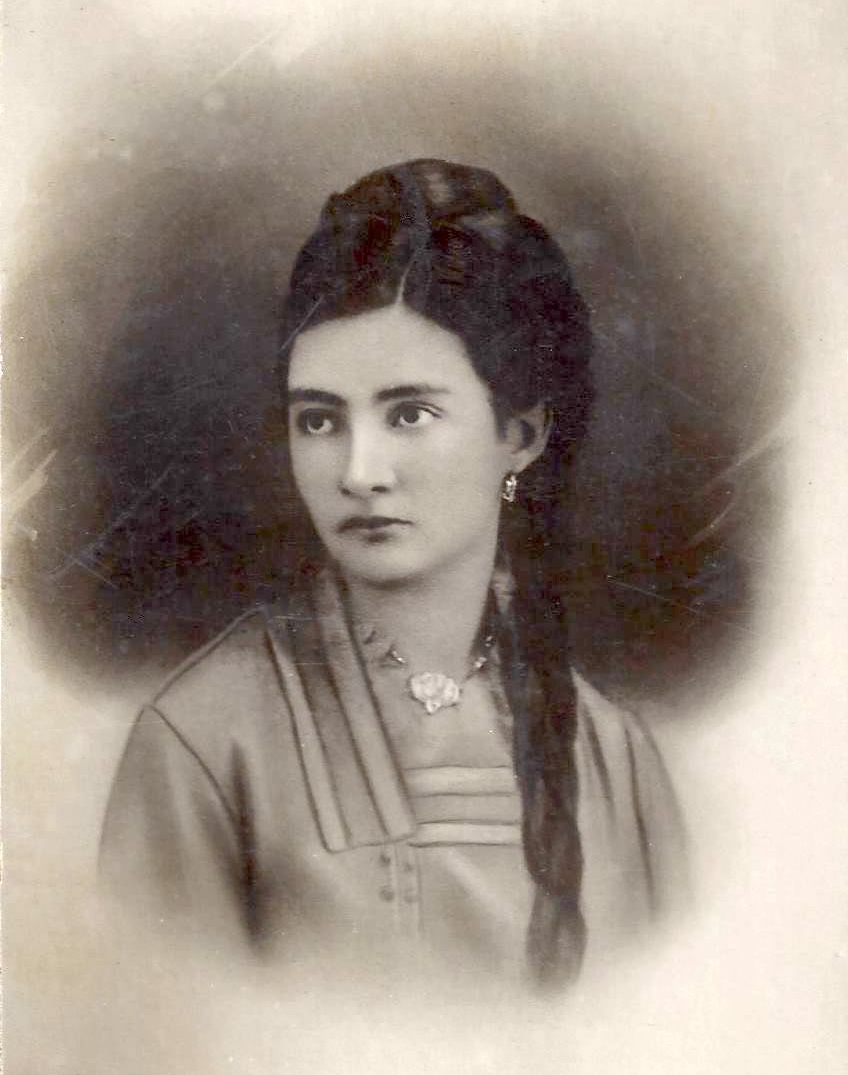
\includegraphics[width=\textwidth]{mariannina}
    \caption[Mariannina Gagliardi]{\textbf{Mariannina Gagliardi}\index[Personaggi]{Gagliardi Mariannina} (1860 - 1882), madre di Stefano. Studiò all'università di Bologna e terminati gli studi si sposò con Natale \index[Personaggi]{Mingazzi Natale}Mingazzi. Morì di tubercolosi a soli 22 anni il 23 settembre 1882 quando Stefano non aveva neanche due anni. Come era solito fare, ai nuovi nati si dava il nome di parenti morti precocemente ed infatti mia nonna prese il nome della madre di Stefano quando nacque nel 1927.  \label{fig:mariannina}}
    %\vspace{-0.3cm}
\end{figure}
%------------------------------------------------------------------------------
%	CAPITOLO 13
%------------------------------------------------------------------------------

\chapter{I paletti bianchi delle strade}
\subsection{I paletti bianchi delle strade}
Per chi non lo sapesse sembrerebbe un'invenzione dell'Azienda Stradale, dovuta allo sviluppo automobilistico, ma così non è. Sotto al governo papale verso il 1850, nella magistratura comunale di Alfonsine si discuteva e si doveva approvare la prima illuminazione pubblica.\\
\indent Il membro \index[Personaggi]{Bagnara Giovanni}Bagnara\footnote{\textbf{Giovanni Bagnara}, fu più volte membro della giunta comunale. Fu il padre di Cassiano\index[Personaggi]{Bagnara Cassiano}, il quale fu vittima di un atto di brigantaggio  da parte della `Ligaza di Trentesì' la sera del 20 novembre 1862 e fu ucciso. Erano i proprietari della casa di Vincenzo Monti} fece la proposta di imbiancare le teste dei pali stradali, perché ciascuno rincasando alla sera avesse un punto di mira per seguire la buona strada.\\
\indent Per molto tempo tutti risero della trovata, ma ora perché è morto da 70 anni... il mondo deve dargli ragione.

\subsection{Le ragazze non devono saper scrivere}
Il \index[Personaggi]{Bagnara Giovanni}Bagnara aveva profondamente radicate le sue convinzioni morali e politiche. Secondo lui le donne non dovevano imparare a leggere e scrivere... perché non scrivessero al fidanzato! La maniera di repressione era, si vede, molto radicale.\\

\subsection{Una vacca morta}
Sempre parlando del nostro uomo che in fondo era buonissimo, diremo ancora.\\
\indent Un giorno un suo contadino gli porta la brutta nuova che gli è morta una vacca. In altre occasioni si sarebbe vivamente accorato\footnote{Dispiaciuto}, per l'affezione che aveva alle bestie e per il danno. Nel caso, non si scompose e rispose:\\
\indent <<L'è l'istes ui aveva la su mitè nec Mingàz\footnote{<<È lo stesso, vi aveva la sua metà anche Mingazzi>>}>>. \\
\indent Si vede che per lui il danno comune era una gioia! E pensare che col Mingazzi\footnote{Probabilmente si parla di \index[Personaggi]{Mingazzi Fedele}Fedele Mingazzi, il nonno paterno di Stefano oppure il padre, Natale Mingazzi} erano amiconi.


 \begin{figure}[htb]
    \centering
    %\vspace{-0.7cm}
    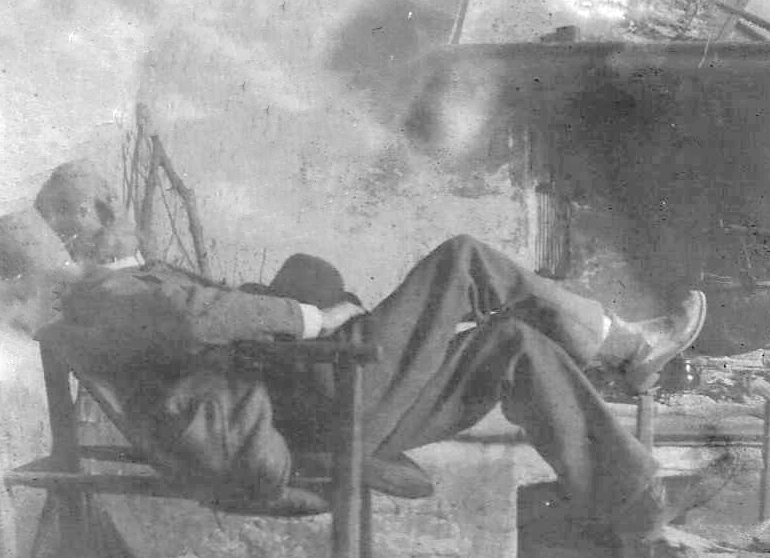
\includegraphics[width=\textwidth]{natalemingazzi}
    \caption[Natale Mingazzi in casa]{\textbf{Natale Mingazzi}\index[Personaggi]{Mingazzi Natale}, il padre di Stefano. Aveva un allevamento di bachi da seta, come ho scoperto leggendo le lettere che la sua futura moglie Mariannina gli inviava da Bologna. In una di quelle lettere si diceva dispiaciuta per il fidanzato sapendo che le larve erano uscite dalla finestra. \label{fig:natalemingazzi}}
    %\vspace{-0.3cm}
\end{figure}
%------------------------------------------------------------------------------
%	CAPITOLO 14
%------------------------------------------------------------------------------

\chapter{Da 15 a 20 paoli di stipendio}
La sede del comune era nel \index[Luoghi]{Borghetto}Borghetto (\index[Luoghi]{Lanconelli (palazzo)}casa Lanconelli ora Martini\footnote{In via Mazzini, nel cosiddetto \textbf{Borghetto}, vi è un lungo caseggiato che viene detto  la ‘Ca d'Pliché'. Pliché era il soprannome dei Martini che vi abitarono e che ne sono ancora i proprietari (2017). Essi erano succeduti alla fine dell'ottocento ai proprietari storici di quell'edificio: i Lanconelli.}). Il consiglio comunale si era radunato in seduta segreta per varie trattazioni e per aumentare lo stipendio al bidello\footnote{Qui inteso come custode.} \index[Personaggiq]{Panciaco (bidello)}Panciaco da 15 a 20 paoli al mese. (\Large \textcal{L 7,50 a 10}\normalfont \normalsize \:)\\
\indent Panciaco per chi non lo sapesse era un omone grande e grosso, molto decorativo, vestito alla Napoleone, con lucerna in testa, falde e spada, per le funzioni della messa cantata della domenica, insieme alla magistratura al completo, con guardie e carabinieri, e per le altre funzioni civili, non escluse le sedute consigliari, che serviva nell'anticamera anche con funzioni di guardiaportone.\\
\indent Al termine della seduta, certo dell'aumento al povero Panciaco, tirava anche l'ombellico dalla consolazione dell'agognato aumento.\\
\indent Con la maestà della divisa e di un Napoleone, spalancò la porta dell'aula consigliare e proruppe con questa esclamazione: <<Ringrazio questa nobile plebaglia!>>\\
\indent Si arguisce che il discorso studiato non lo seppe dire o si confuse.

 \begin{figure}[htb]
    \centering
    %\vspace{-0.7cm}
    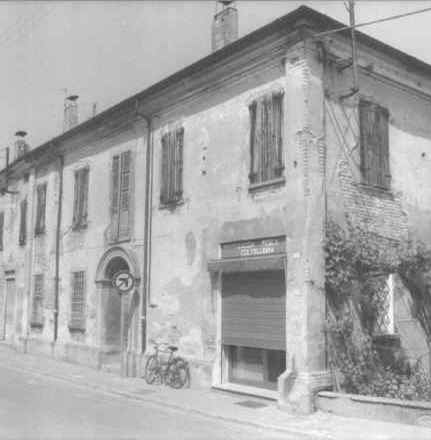
\includegraphics[width=\textwidth]{casamartini}
    \caption[Caseggiato Martini - Lanconelli]{Il \textbf{caseggiato Martini - Lanconelli}. Lanconelli fu una delle più ricche famiglie che fu nel territorio alfonsinese fin dai primi dell'ottocento. Prima di questa data non si hanno notizie della presenza di tale famiglia ad Alfonsine. Probabilmente erano lughesi e, con l’avvento di Napoleone e l'occupazione francese dei territori anche nella Bassa Romagna, riuscirono ad approfittarne. \label{fig:casamartini}}
    %\vspace{-0.3cm}
\end{figure}
%------------------------------------------------------------------------------
%	CAPITOLO 15
%------------------------------------------------------------------------------

\chapter{Alt, chi va là}
\index[Personaggi]{Bigano (fabbro)}Bigano, fabbro di professione, era un acceso liberale del 1859, mangiacristi e mangiapreti, fremeva per poter trasportare l'incudine sull'altar maggiore, diceva. Caporale della guardia nazionale si scalmanava da vero bravaccio\footnote{Chi con parole e portamento minacciosi e arroganti cerca di imporsi più all'attenzione che alla volontà altrui}.\\
\indent Una sera del Maggio 1859 era caporale caposto al quartiere della guardia nazionale, nel Corso e nella casa ex caserma dei gendarmi pontefici, poi Lugaresi, De Maria, ora \index[Luoghi]{Lugaresi (palazzo)}Dopolavoro\footnote{\textbf{Palazzo Lugaresi} era in corso Garibaldi, non lontano dal Credito Romagnolo. Era l'antico palazzo del Cav. Aristide Lugaresi, farmacista e consigliere comunale, padre di Santina e nonno materno di Antonio Camanzi, che ne divenne l'unico erede negli anni '30. Rimase distrutto durante la seconda guerra mondiale}.\\Ad un tratto sentì uno scalpittio di cavallo che veniva dal \index[Luoghi]{Ponte Nuovo}pontenuovo\footnote{Si tratta del ponte sulla via Reale, all'incrocio con corso Garibaldi}. Il caldanzoso caporale, fu pronto, al buio, a gridare:\\
\indent "Alt chi va là".\\
\indent Rispose una voce: "Ufficiale austriaco".\\
\indent Non ci volle altro, senza di nulla più curarsi il nostro valoroso caporale, abbandonò armi, berretto e via di corsa per la porta di dietro per i campi, subito imitato dai suoi militi. Si fece vedere solamente quando la burrasca fu passata da qualche giorno.\\
\indent Chi era stato? All'insaputa di tutti e senza preavvisi era arrivata l'avanguardia austriaca, della intera guarnigione di Ancona, che aveva sgombrato della fortezza per recarsi sui campi Lombardi alla guerra.\\
\indent Per chi non lo sapesse il corpo austriaco era forte di seimila uomini, aveva disposto l'avanguardia alla \index[Luoghi]{Tosca}Tosca\footnote{Zona a ridosso dell'incrocio tra Via Reale e Via Valeria}, sul \index[Luoghi]{Ponte Nuovo}Ponte Nuovo vari pezzi di cannone ai quali erano addetti gli artiglieri sempre con la miccia accesa e pronti al fuoco.\\
\indent Figurarsi il terrore della popolazione allo spettacolo insolito, molto di più perché gli austriaci si erano fissati che in Alfonsine fosse nascosto \index[Personaggi]{Garibaldi Giuseppe}Garibaldi e lo cercavano affannosamente. \\
\indent Si dice anche che un tale, sfuggito alla memoria, alle minacce di un austriaco, fece finta di soddisfarlo, lo condusse nella sosta del fiume, se lo fece camminare innanzio e quando fu ai limiti della scarpata, con una spinta lo mandò a ruzzolare nell'acqua e fuggì a gambe levate per sottrarsi al pericolo.\\
\indent Il generale austriaco dormì nella \index[Luoghi]{Lugaresi (palazzo)}casa Lugaresi.\\
\indent Furono requisiti generi, carri, carrettieri e contadini per trasportare gli equipaggiamenti e servizi austriaci fino all'altra tappa di \index[Luoghi]{Argenta}Argenta.

 \begin{figure}[htb]
    \centering
    %\vspace{-0.7cm}
    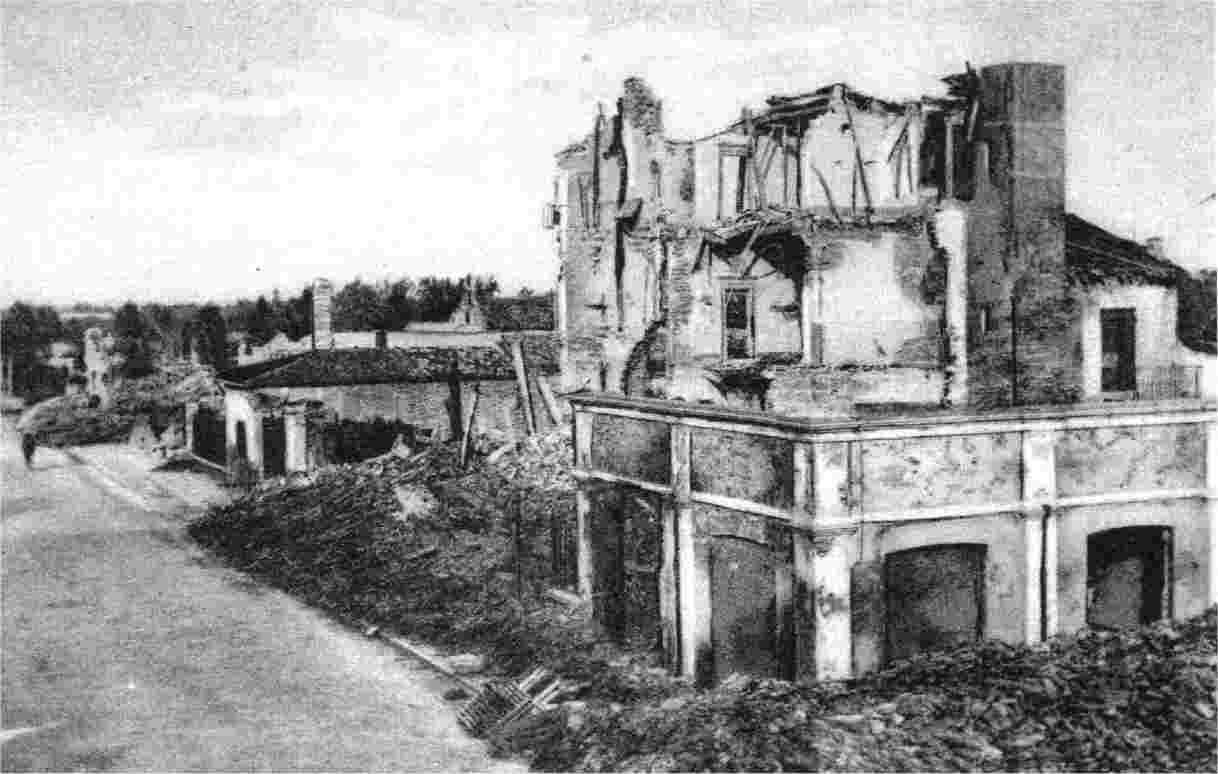
\includegraphics[width=\textwidth]{palazzolugaresi}
    \caption*{Palazzo Lugaresi distrutto dopo la guerra.\label{fig:palazzolugaresi}}
    %\vspace{-0.3cm}
\end{figure}

%------------------------------------------------------------------------------
%	CAPITOLO 16
%------------------------------------------------------------------------------

\chapter{Come si può cambiare bandiera}
I più arrabbiati papalini del paese erano \index[Personaggi]{Bagnara Giovanni}Bagnara, del quale ci siamo occupati, il fabbro \index[Personaggi]{Cappelli Paolo}Paolo Cappelli della \index[Luoghi]{Tosca}Tosca ed il vecchio \index[Personaggi]{Bartolotti Francesco}Bartolotti\footnote{\textbf{Bartolotti Francesco} fu un consigliere comunale insieme a \textbf{Giovanni Bagnara} attorno al 1855}, che abitava al \index[Luoghi]{Cortilazzo}Cortilazzo, poco prima della \index[Luoghi]{Tosca}Tosca. Passando per la strada gli austriaci, in parecchi ebbero necessità urgente di soddisfare certe occorrenze corporali e si rifugiavano nel cortile del \index[Personaggi]{Bartolotti Francesco}Bartolotti.\\
\indent Non ci volle altro! Prima così fermo nelle sue idee papaline, austriacanti reazionare e resistenti alle minacce liberali... il vecchio \index[Personaggi]{Bartolotti Francesco}Bartolotti disertò, per questa offesa al suo suolo, il campo e passò nel campo liberale in armi e bagaglio!\\
\indent I suoi compagni \index[Personaggi]{Bagnara Giovanni}Bagnara e \index[Personaggi]{Cappelli Paolo}Cappelli non gliela perdonarono e specialmente quest'ultimo, cliente e amico del magnano\footnote{Artigiano che esegue minuti lavori in ferro} \index[Personaggi]{Giovacchino}Giovacchino (trentino di nascita) quando passava per andare o tornare a piedi per recarsi nel Trentino lo chiamava e gli diceva:\\
\indent <<Juvachìn a iei i fradèl a \index[Luoghi]{Pontelagoscuro}Pont Legscur\footnote{<<Giovacchino, ci sono i fratelli austriaci a Pontelagoscuro?>> - Pontelagoscuro è una frazione del comune di Ferrara}?>>\\
\indent Juvachìn rispondeva: <<Oh, sè\footnote{<<Oh, si>>}>>.\\
\indent \index[Personaggi]{Cappelli Paolo}Cappelli: <<Alora disìi cossa chi fa chin ven in qua ad amazé tot sti vigliac d'Italièn\footnote{<<Allora dite(chiedete) loro che cosa fanno che non vengono qua ad ammazzare questi vigliacchi d'Italiani>>}>>.\\
\indent Poi grattava e si calcava in testa la papalina, riprendeva il lavoro per consolare la sua ira.



%-------------------------------------------------------------------------------
%	CAPITOLO 17
%-------------------------------------------------------------------------------

\chapter{Tre teste da capestro tutte e tre}
Il vecchio conte \index[Personaggi]{Foschini Camillo (conte)}Foschini era padrone ed abitava la casa \index[Luoghi]{Alberani (palazzo)}Alberani\footnote{\textbf{Palazzo Alberani}, La casa della famiglia del Dott. \index[Personaggi]{Alberani Anselmo}Anselmo Alberani, uno dei più ricchi proprietari terrieri di Alfonsine, in via Reale (dove oggi c'è la fabbrica di trasformazione “Contarini”). Era il padre di Alberto Alberani, che fu sindaco di Alfonsine.}. Una sera faceva la partita nella camera da pranzo, con amici, tra i quali \index[Personaggi]{Don Salvatori Ruggero}Don Ruggero. Era irrequieto, si contorceva sulla sedia, sembrava sugli spini. Accese un lume ad olio, disse agli amici: <<Vengo subito.>> e sparì. È da dire che il vecchio conte era un accanito papalino, mentre suo figlio \index[Personaggi]{Foschini Stefano}Stefano era liberale carbonaro\footnote{La Carboneria è stata una società segreta rivoluzionaria italiana, nata nell'allora Regno di Napoli durante i primi anni dell'Ottocento su valori patriottici e liberali.} acceso. \\
\indent In una camera superiore della casa erano a confabulare \index[Personaggi]{Farini Luigi Carlo}Luigi Carlo Farini\footnote{\textbf{Luigi Carlo Farini} (Russi, 22 ottobre 1812 – Quarto, 1 agosto 1866) è stato un medico, storico e politico italiano, per breve tempo Presidente del Consiglio dei ministri del Regno d'Italia tra il 1862 e il 1863.} il futuro dittatore e Ministro, \index[Personaggi]{Strocchi Girolamo}Momo Strocchi\footnote{\textbf{Strocchi Girolamo}, figlio di \index[Personaggi]{Strocchi Dionigi}Dionigi Strocchi che era stato un letterato, grecista e latinista italiano, amico di \index[Personaggi]{Monti Vincenzo}Vincenzo Monti. Nasce da Dionigi nel 1812. Da sempre cospiratore anche se mai vicino alle posizioni mazziniane estreme, è costretto ad esulare nel 1843. Rientrato a Faenza nel 1848 è capitano con il battaglione di volontari faentini che combatte a Vicenza e l'anno successivo viene arrestato dalle autorità pontificie. Nel 1850 è nominato colonnello della Guardia Nazionale. Con l'Unità d'Italia è più volte consigliere ed assessore comunale. Muore a Faenza nel 1885.} liberale faentino ed il conte \index[Personaggi]{Foschini Stefano}Stefano\footnote{Farini, Strocchi e Foschini erano tre rivoluzionari liberali che parteciparono al moto antipapalino di Romagna del 1843.}. Il vecchio conte padre si mise ad origliare dietro la porta i colloqui. Udito che ebbe che parlavano di politica, aprì la porta come un fulmine, col lume nella sinistra, la destra e l'indice teso si rivolse ai presenti indicandoli: <<Uno, due, tre, tre teste da capestro tutte tre\footnote{<<Tre teste da legare/impiccare>>}>>.\\
\indent Voltò le spalle, richiuse la porta e discese in fretta dagli amici, ridendo e dicendo: <<Credevo che facessero firmare cambiali a mio figlio... invece parlano di politica!>>\\
\indent Dopo il temporale era venuto il sereno nella faccia del vecchio conte, le cambiali erano uno sturbo\footnote{Scompiglio} forte... trasgredire ai suoi principi politici era cosa sopportabile!

 \begin{figure}[htb]
    \centering
    \vspace{-0.2cm}
    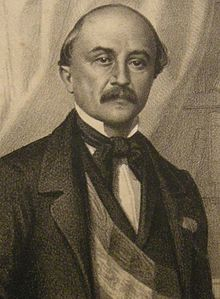
\includegraphics[width=0.7\textwidth]{farini}
    \caption[Luigi Carlo Farini]{Luigi Carlo Farini\\ Russi, 22 ottobre 1812 - Quarto, 1 agosto 1866\index[Personaggi]{Farini Luigi Carlo}\label{fig:farini}}
    \vspace{-0.4cm}
\end{figure}
%-------------------------------------------------------------------------------
%	CAPITOLO 18
%-------------------------------------------------------------------------------

\chapter{Benedette le tue gambe}
Nel 1849 tra \index[Luoghi]{Alfonsine}Alfonsine e \index[Luoghi]{Fusignano}Fusignano si era mobilitata una compagnia di guardie nazionali, comandata da capitano avvocato \index[Personaggi]{Santoni Pietro (capitano, avvocato)} Santoni di Fusignano. Questo signore capitano era persona greve di peso, con una gran pancia e due gambe esili, come dicono.\\
\indent In rinforzo all'esercito regolare questa compagnia armata di schioppi da caccia, allora non avevano armi da guerra, pistole ecc. era stata spinta fino al Piave\footnote{Il Piave è un fiume italiano, che scorre interamente in Veneto nell'omonima valle} insieme all'esercito operante. Su questo fiume, sacro alla patria a sinistra erano gli austriaci, a destra gli Italiani.\\
\indent La brava compagnia della nostra guardia, parte era di guardia, parte a riposo sui cascinali\footnote{Gruppo di casolari in aperta campagna, organizzati o no come cascine.} vicini, quando un brutto mattino ebbe un brusco risveglio. L'artiglieria aveva smantellato due nostri pezzi di artiglieria, minacciava l'attacco delle fanterie. Stordite, le povere guardie si diedero alla fuga. I dormienti si svegliarono e poco rendendosi conto dell'accaduto seguirono i fuggiaschi.\\
\indent Tra le guardie militava anche un certo \index[Personaggi]{Taglioni}Taglioni di qui, famoso cacciatore addomesticatore di cani trifolai\footnote{Cani da tartufo}, secco, smilzo e celebre corridore. Il \index[Personaggi]{Taglioni}Taglioni dormiva su di un cascinale, al frastuono si svegliò, si trovò solo, solo, impaurito ancora di più perché sperduto, prese la fuga, raggiungendo or l'uno or l'altro dei commilitoni che sorpassava con una velocità elastica da saetta, senza curarsi di loro. Dopo poco raggiunse il capitano\index[Personaggi]{Santoni Pietro (capitano, avvocato)}, e quando lo ebbe sorpassato si sentì da questo chiamare, con la invocazione: <<E mi Taiòn, banadèt al tu gamb\footnote{<<Il mio Taglioni, benedette le tue gambe>>}>>.\\
\indent L'invocato, si soffermò e degnò di una frettolosa risposta curiosa il suo capitano: <<A se sgnor me m'avèg da què\footnote{<<Si signore, io me ne vado da qui>>}>>\\
\indent Accompagnò la detta con un colpo della mano sinistra sull'avanbraccio destro, molto significativa, e via nuovamente di corsa.\\
\indent Intanto il povero capitano\index[Personaggi]{Santoni Pietro (capitano, avvocato)}, ansante e sbuffante, col sudore caldo e freddo dell'emozione zampettava per mettere la maggior distanza tra di lui e l'odiato nemico.\\
%-------------------------------------------------------------------------------
%	CAPITOLO 19
%-------------------------------------------------------------------------------

\chapter{La commedia di Ciro - In pensione}
\subsection{La commedia di Ciro}
\index[Personaggi]{Bonfiglioli Ciro}Ciro Bonfiglioli\footnote{\textbf{Ciro Bonfiglioli}, di lui mi è stato raccontato che per vendicarsi dello scarso stipendio, insegnava ai suoi alunni che 2+2=3.}, maestro elementare, poeta, cacciatore, venditore di pistole, fucili, orologi, per 50 anni è stato una tipica macchietta\footnote{Un personaggio particolare}.\\
\indent Si vedeva un gran testone con due protuberanze sulla testa, un naso ammaccato dal quale si staccavano le narici, sotto un pelame di baffi biondi che gli coprivano una bocca sdentata, un mento sporgente, due occhi che si chiudevano a membrana come un giocattolo di Norimberga\footnote{Città tedesca famosa per i giocattoli}. Sotto un corpo lungo, lungo da persona alta e due gambine corte da fanciullo.\\
\indent In primavera vendeva i vestiti d'inverno e comprava a credito quelli d'estate. Spendeva lo stipendio, depurato dall'ammortamento dei debiti, nei primi tre giorni del mare e per gli altri 27 vivacchiava a credito presso i contadini, a riparare orologi, scrivere lettere od altro servizio. \\

\indent Aveva una grande facilità di verseggiare\footnote{Era un abile oratore}, era un gaudente\footnote{Ricercatore assiduo degli agi e dei piaceri che la vita può offrire}, rideva sempre, pigliava tutto in ischerzo, ma se ne aveva a male seriamente quando i ragazzi dicevano: \\\\
\textcal \Huge
	\centerline{Ciro, Ciro pesta pevar}
	\centerline{tu l'amzeta e pu dam da bevar}\normalfont \normalsize\footnote{"Ciro, Ciro pesta pepe, prendi la mezzetta(di vino) e poi dammi da bere"}
\index[Personaggi]{Bonfiglioli Ciro}

Ciascuno ha le sue debolezze, come poteva essere quello dello scrivere, ma però era una cosa amena\footnote{Dilettevole, divertente} per lui e per tutti. \\
\indent Verso il 1886 c'era qui nell'unico teatro, \index[Luoghi]{Teatro Camerani}Camerani\footnote{\textbf{Teatro Camerani}, che si trovava alla destra del Senio, dove oggi c'è la casa Natali subito sotto la rampa. Tale teatro fu costruito probabilmente nei primi dell'800 da \index[Personaggi]{Camerani Giovan Antonio (governatore)}Giovan Antonio Camerani, avvocato e Giudice di Pace, figlio di Matteo Camerani, fattore della famiglia Spreti che aveva sposato la sorella di Vincenzo Monti, Maria Cristina} la compagnia drammatica \index[Personaggi]{Catastini Cesare}Cesare Catastini. Il nostro Ciro\index[Personaggi]{Bonfiglioli Ciro} scrisse la commedia: "Caccia, bugie, amore". La recita venne troncata da una salva\footnote{Insieme di più colpi sparati da più bocche da fuoco} di fischi ed il telone calò.\\
\indent Il capo comico venne alla ribalta scusando la compagnia e tenendone alto il merito e scagliandosi contro quel cane dell'autore della commedia.\\
\indent Fu applaudito e scusato. Al nostro Ciro\index[Personaggi]{Bonfiglioli Ciro}, bruciava la sconfitta artistica ed agli applausi al capo comico, ardì comparire alla ribalta annunziando: <<Quei cani dei commedianti hanno rovinato la mia commedia>>.\\
\indent Una salva di fischi lo accolse. Dopo seguì una lunga invettiva tra il capo comico e l'autore, con godimento del pubblico che ne fece una carnevalata e la commedia si può dire che fu esilarante e bellissima... a telone calato. 

\subsection{Ciro in pensione}
L'ispettore scolastico \index[Personaggi]{Zaccaria Antonio}Zaccaria\footnote{Cav. prof. \textbf{Antonio Zaccaria} (1842 - 1905), ispettore scolastico per il circondario di Ravenna}, uomo alto, con barba, vestito di nero, tutto compreso del suo ufficio, col cavallo di S. Francesco\footnote{Modo di dire: `andare a piedi'} un giorno si recò al \index[Luoghi]{Fiumazzo}Fiumazzo a visitare la scuola del maestro Ciro\index[Personaggi]{Bonfiglioli Ciro}.\\
\indent Un baccano infernale si sentiva nell'aula. L'ispettore bussa, ribussa, seguita il baccano e nessuno risponde.\\
\indent Pensa l'ispettore che nell'aula non ci sia il maestro, si decide, apre la porta ed entra.\\
\indent Che spettacolo! i ragazzi giocavano, spaccavano legna, uno faceva la minestra sul tavolo del maestro, e sullo stesso tavolo era una mezzetta di vino, un bicchiere vuoto ed il maestro chino e addormentato.\\
\indent All'entrata dell'ispettore, col silenzio che fecero i ragazzi, il maestro si alzò, si stirò, arrossì, scattò in piedi, cominciò ad urlare all'ispettore: <<Ah, lei viene per rovinarmi, fuori, fuori...>> e lo spinse fuori dalla porta.\\
\indent Pochi giorni dopo Ciro\index[Personaggi]{Bonfiglioli Ciro} fu collocato in pensione d'autorità con 40 lire al mese.

\subsection{Poesie}
Quando il povero Ciro\index[Personaggi]{Bonfiglioli Ciro} era in bolletta mandava poesie ad autorità, persone facoltose, per essere aiutato.\\
\indent Una volta mandò una poesia a Sua Maestà la \index[Personaggi]{Margherita Maria Teresa Giovanna di Savoia}Regina Margherita\footnote{Margherita Maria Teresa Giovanna di Savoia (Torino, 20 novembre 1851 – Bordighera, 4 gennaio 1926) come consorte di re Umberto I} ed un'altra al Carlino. Il Carlino la mise nella cronaca burlesca e Ciro se ne ebbe a male e rispose al Carlino: <<Per una poesia la Regina mi ha mandato cinquanta lire per il delegato di P. Sicurezza\footnote{Pubblica Sicurezza, complesso di apparati, autorità e strutture preposte alla tutela dell'ordine pubblico e all'incolumità delle persone.}>>\\
\indent Subito il Carlino pubblicò: <<Sua Maestà la Regina Margherita, ha mandato il delegato di Pubblica Sicurezza dal signor Ciro Bonfiglioli\index[Personaggi]{Bonfiglioli Ciro} con ordine di arrestarlo e metterlo per sempre in prigione se ardirà di scrivere altre poesie.>>\\
\indent In altra occasione il nostro poeta andava a sciacquare i pennelli da un imbianchino, pittore ed esclamò: <<Non vedi che questi ragazzi dipinti sembrano gravidi!>>\\
\indent Il pittore fece una zirudella\footnote{Filastrocca} a Ciro per risposta e Ciro altre al pittore, e della girale solo si ricorda\footnote{Il pittore e Ciro si scambiavano filastrocche e dello scambio di `offese' si ricorda solamente quanto segue}:\\\\
\textcal \Huge
	\centerline{Quegli è Morandi, vate e pittore}
	\centerline{carnevalesco decoratore ecc...} 
\normalfont \normalsize
\\

In altra occasione, tra le tante inviò una poesia, intenta ad avere un sussidio da un agente di campagna. \\
\indent Questo, furbo, rispose: <<Caro Ciro, ho venduto la vostra poesia, ho preso lire zero, e zero ve li mando>>.\\
\indent Il nostro poeta rispose: <<C. O. agente di M... è stato un bravo topo - nei grandi magazzini - l'anghusto somarone\footnote{Somarone meschino} ecc...>>\\
\indent Così queste facezie divertivano il paese, nelle more\footnote{Solite} degli avvelenamenti politici. 

































%

%-------------------------------------------------------------------------------
%	CAPITOLO 20
%-------------------------------------------------------------------------------

\chapter{Gli artigiani}

A dire il vero in Alfonsine non furono molti, si ricorda una epigrafe\footnote{Testo esposto pubblicamente su un supporto di materiale non deperibile} che andò per varie generazioni e cioè:
\\\\
\textcal \Huge
	\centerline{Gramantieri Tomaso}
	\centerline{e car fasè}
	\centerline{Santoni Proculo}
	\centerline{ul piturè}\normalfont \normalsize \footnote{Tomaso Gramantieri fece il carro, Proculo Santoni lo pitturò - Mi è stato detto da \index[Personaggi]{Pasi Adis}Adis Pasi che in una casa dietro alla \index[Luoghi]{Villa Marini}Villa Marini, vi era questa epigrafe che però riportava una frase leggermente diversa: "Checco Gramantieri e car fasè, Brocul e Santoni il piturè"}

\index[Personaggi]{Gramantieri Tomaso}\index[Personaggi]{Santoni Proculo}
%-------------------------------------------------------------------------------
%	CAPITOLO 21
%-------------------------------------------------------------------------------

\chapter{Uno spuntino}
Il povero cav. \index[Personaggi]{Zaccaria Antonio}Antonio Zaccaria, faentino, ispettore delle scuola, persona compitissima\footnote{Ben educata, gentile e discreta}, impeccabilmente vestito di nero, barba bianca, alto, compreso della sua missione, moralissimo più realista del Re, un vero tipo e modello di funzionario. Questo l'uomo.\\
\indent Un giorno usciva dalla scuola del \index[Luoghi]{Borgo Gallina}Borgo Gallina\footnote{Detto anche Borgo Fratti, è la zona a ridosso del fiume in vi Antonio Fratti}, sul mezzogiorno, incontra una vecchietta, con affabilità, sottovoce e gran circospezione, le dice: <<Buona donna, spendendo poco si potrebbe fare uno spuntino>>.\\
\indent La vecchia, sorpresa dal fare circospetto e misterioso del cavaliere, e molto a digiuno della lingua di Dante, inarca le ciglia, si mette le mani sulla cintola e come suol dire si inalbera ed acerba risponde: <<Cossa, me a so vecia, mo d'al cos che l'è an no mai fat e mai aiò tnu man...\footnote{<<Cosa? Io sono vecchia, ma delle cose come quella non ne ho mai fatte e mai ne ho tenuto mano>>}>>.\\
\indent Il povero ispettore allibì, temendo di sollevare uno scandalo per l'ignoranza della vecchia, si riprese ed affascinante rispose: <<Oh! Oh! Buona donna che cosa avete mai capito! Voglio dire se si possono mangiare due ova al tegame!>>\\
\indent La vecchia, schiarita nelle idee e nella faccia, replicò: <<Mo alora u m'à da dì che vò magné\footnote{<<Ma allora mi deve dire che vuol mangiare>>}>>\\
\indent E le cose si accodarono tra la vecchia e il cavaliere.

%-------------------------------------------------------------------------------
%	CAPITOLO 22
%-------------------------------------------------------------------------------

\chapter{La parola - Virtù del vino}
\subsection{La parola}
Si trattava di un buon diavolo, del tipo più vecchio che nuovo, per i suoi tempi. G. \: \: sensale da vino\footnote{Mediatore in contrattazioni di prodotti enologici}, reduce delle patrie battaglie era abbastanza introdotto\footnote{Disponeva di conoscenze o relazioni utili allo svolgimento della propria attività}, quantunque non fosse troppo magniloquente\footnote{Sebbene non fosse un gran oratore}.\\
Un giorno nella cantina \index[Personaggi]{Mingazzi Fedele}Mingazzi\footnote{Fedele Mingazzi, nonno di Stefano Mingazzi, fu il veterinario del pubblico macello di Alfonsine. Investì numerose cariche nel Comune}, certo \index[Personaggi]{Allegri}Allegri di \index[Luoghi]{Glorie}Glorie doveva comprare una partita di vino. Il venditore chiedeva novanta lire, l'acquirente storceva il collo e premetteva meno, il sensale, con voce da basso profondo chiede: "La parola a me", prende le mani del venditore e dell'acquirente e con le sue le stringe fortemente imprimendo il colpo, finale solito, per la conclusione e sillaba: "Zdot scud\footnote{"Diciotto scudi". Equivalevano a 90 Lire: con l'avvento del sistema decimale nella monetazione dell'Ottocento il termine scudo venne utilizzato per la moneta da 5 lire in argento. Monete di questo modulo sono rimaste in uso fino alla prima guerra mondiale}".\\
Una risata accolse tale sproposito, ma il contratto si fece su altre basi.
\subsection{Virtù del vino}
È sempre il nostro uomo che parla.\\
Un giorno parlando con una maestra chiese: "L'an ha mai avù fiùl\footnote{"Non ha mai avuto figli?"}?"\\
La maestra: "No."\\
Il nostro G. \:\:\:\:: "Alora cla beva de ven négar gros sl'in vó mètar in sê\footnote{"Allora beva del vino nero grosso se ne vuol mettere insieme"}".\\
Farmacisti e medici aprite questa ricetta alla terapia. 


%-------------------------------------------------------------------------------
%	CAPITOLO 23
%-------------------------------------------------------------------------------

\chapter{L'istrumento di divisione - tre paoli}

Questo capitolo è presente nell'indice, ma non vi è nei manoscritti. Non so se Mingazzi lo scrisse altrove ed è andato perduto, oppure se si è dimenticato completamente di scriverlo. Non lo scopriremo mai.

 \begin{figure}[htb]
    \centering
    %\vspace{-0.7cm}
    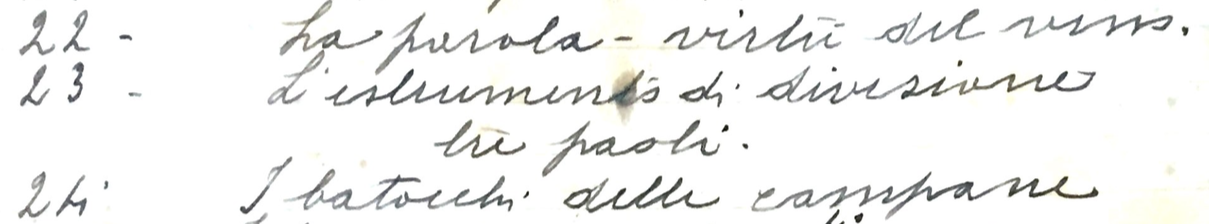
\includegraphics[width=\textwidth]{capitolo23}
    %\vspace{-0.3cm}
\end{figure}
%-------------------------------------------------------------------------------
%	CAPITOLO 24
%-------------------------------------------------------------------------------

\chapter{I batocchi delle campane}
Verso il 1870 serpeggiava in paese ancora la lotta dei liberali contro il partito papalino, che aveva il suo esponente nei preti. I preti erano i più forti di numero , perché contavano sull'elemento femminile, sui contadini, i quali mal sopportavano le ultime schioppettate della guerra d'indipendenza nazionale, e la leva nuovamente introdotta.\\
\indent Per gente che fugge il rumore e bada solamente ai propri interessi, le vecchie idee, solo perché contrarie al nuovo ordine erano un vangelo, la sacrestia e la chiesa el tempio della ribellione contro le novità. Bastava un rintocco di campana per radunare il popolo tutto a dispetto dell'elemento liberale. \\
\indent Si era giunti al carnevale, l'elemento liberale voleva scialarsela\footnote{Godersela, spassarsela}, ballare anche la seconda mezzanotte del martedì grasso che cadeva in Quaresima. Dal canto della chiesa come contromisura erano state chiamate ed in funzione le sacre missioni.\\
\indent Questo fu il colmo! Le ragazze morigerate allora disertarono i festini, schivarono i fidanzati o come suol dirsi i filarini, che forse avevano pensato per un anno di avere nelle braccia le loro belle, almeno nel ballo.\\
\indent Maledette campane! Oltre che stordire gli abitué della piazza chiamavano alla chiesa ed alle prediche il bel sesso, e popolo alla mattina, pomeriggio, sera, con relative confessioni, comunioni... per tenerle sempre in devozione ed in santità lontano dai peccati. Figurate l'ossessione degli irati filarini-liberali a... spasso per la forzata disoccupazione.\\

Il vecchio campanaro \index[Personaggi]{Barabisa (campanaro)}Barabisa come sempre, va a suonare l'Ave Maria del giorno, ma tira, tira, credeva di avere perduto la forza e di non suonare le campane. Bisognò che rischiarasse la mente sonnolenta per convincersi... di essere ancora lui... in forza.\\
\indent Che era? Che non era?\\
\indent Avevano, nella notte, portato via i batocchi delle campane!\\
\indent La voce si diffuse in un baleno, tutti furono mobilitati alla ricerca affannosa dei sacri batocchi in ogni angolo. Si pescavano anche nelle sabbie del fiume, e un colpevole che assistiva a questa curiosa pesca... si mordeva... e brontolava... <<è non sono mica lì>>.\\
\indent Finalmente, dopo tre giorni il detto \index[Personaggi]{Il Dio Scalzo}Dio Scalzo, un fanatico portastendardo delle confraternite, un poveraccio, arrivò a pescare tra le acque e sabbie del fiume i rubati batocchi e trionfò in nome della fede, in odio ai nemici ed ai due paoli al giorno per la ricerca\footnote{Trovati i batacchi delle campane, esultò anche per i soldi guadagnati per la ricerca}.\\
\indent Per quel carnevale... fu una quaresima per gli innamorati\footnote{Mentre le campane erano fuori uso, i ragazzi potevano festeggiare il carnevale liberamente}.
 \begin{figure}[htb]
    \centering
    \vspace{-0.2cm}
    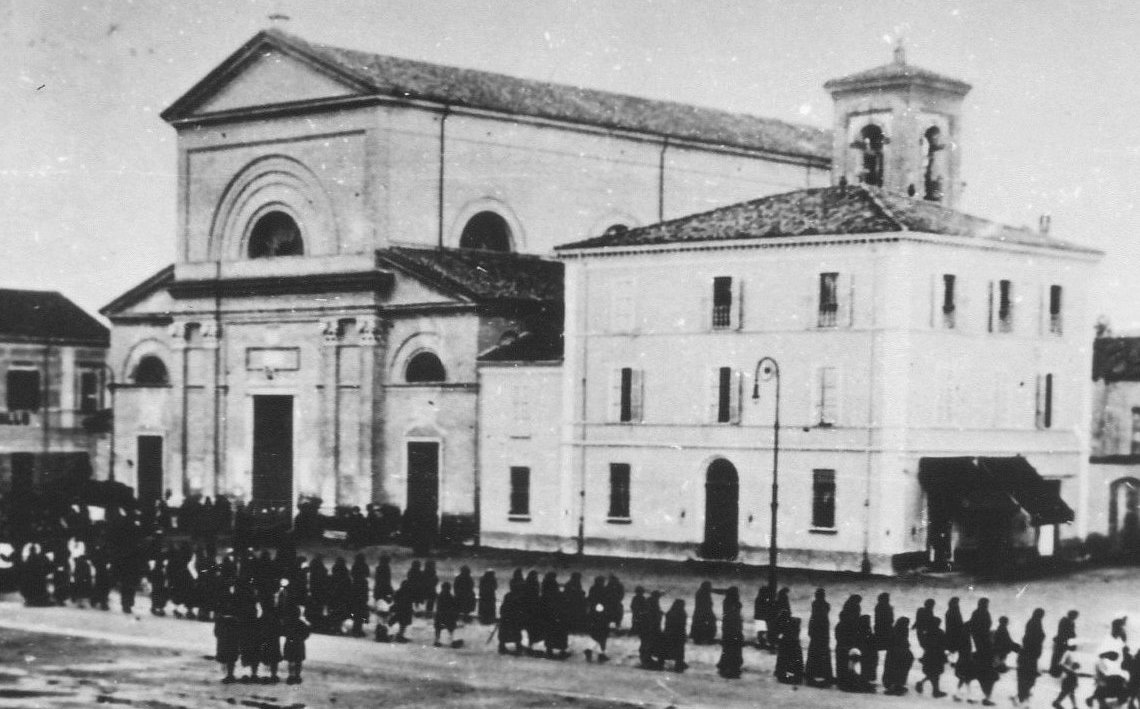
\includegraphics[width=\textwidth]{chiesa}
    \caption*{La chiesa Santa Maria in Piazza Monti\label{fig:chiesa}}
    \vspace{-0.2cm}
\end{figure}






















%
%-------------------------------------------------------------------------------
%	CAPITOLO 25
%-------------------------------------------------------------------------------

\chapter{I funerali di 1\textsuperscript{a}, 2\textsuperscript{a}, 3\textsuperscript{a}, 4\textsuperscript{a} classe}
Nella chiesa parrocchiale avevano sede le confraternite femminili e maschili che erano le più importanti. Vi era la compagnia del sacco, perché i suoi membri portavano una cappa con cappuccio nero e neanche la punta del naso lasciavano scorgere. \\
\indent La compagnia di S. Antonio, con saio bianco e mantellina verde. Altre confraternite tra le quali quella del SS. Sacramento i cui membri portavano la cappa bianca e sopra una mantellina rossa. Qualche vecchio esemplare si può ancora vedere di quest'ultima compagnia, tra i vecchi e nelle grandi funzioni religiose.\\
\indent La compagnia di S. Antonio possedeva le bare per il trasporto a spalla dei defunti. I confratelli non pagavano nulla per i loro funerali: pensava la compagnia. La compagnia poi mandava ai funerali dei confratelli una sua rappresentanza numerosa vestita dei caratteristici costumi e con gonfalone\footnote{Stendardo della confraternita}.\\
\indent Il funerale si disponeva con chierico e crocifisso in testa e clero. Poi venivano i confratelli in due fila, ai margini stradali, con torcia in mano e oranti. In mezzo della strada erano i gonfaloni delle confraternite. Poi la bara ed i portatori, sempre in numero di otto, 4 portatori e 4 ricambi. E dietro i parenti, amici, ecc. La bara nuova era la migliore con un grande panno nero arabescato, con teschio tibie ecc, ed era riservata ai funerali di 1\textsuperscript{a} classe. \\
\indent La bara vecchia era più leggera, più stretta, portava un panno meno lussuoso ed era per i funerali di 2\textsuperscript{a} classe. Vi erano adibiti 4 portatori.\\
\indent Per i funerali di terza classe vi era il cataletto, specie di barella, con sopra un coperchio nero con sopra dipinta la morte e la croce. Serviva per i morti ed anche per portare i vivi malati all'ospedale. I portatori erano due, senza ricambio, e per molti anni furono \index[Personaggi]{Loz}Loz, bracciante, pestatore del pepe nel mortaio dei vari negozi, e \index[Personaggi]{Paulon, e Sandron d'Schenal}Sandron d'Schenal, anelante\footnote{Aspirante} affossatore del becchino. Erano pagati 15 baiocchi ciascuno. \index[Personaggi]{Loz}Loz e Paulon\footnote{Qui Mingazzi lo chiama Paulon, sopra Sandron. Sono sicuramente la stessa persona e probabilmente Paulon veniva anche chiamato "e sandron ad Schenal"}, staccavano la loro tracolla dalla carriola, la infilavano nelle stanghe del cataletto e via per la loro opera funebre.\\
\indent Il clero era numeroso per i funerali di 1\textsuperscript{a} classe, lo sbattocchiamento delle campane grande, ceri ecc. Per quelli di seconda il clero era meno numeroso, meno i ceri ecc. Per la terza classe, un cappellano, in servizio gratuito ed il chierico in testa.\\
\indent Al cimitero era un caso quasi impossibile che non succedesse una lite e non venissero alle mani i portatori, o parenti del morto con il prepotente becchino (\index[Personaggi]{Giuseppe `Iusef' (becchino)}Iusef) il quale si credeva nelle sue funzioni un sovrano dispotico. Una volta aveva, questo malvagio, calato nella fossa un morto bocconi\footnote{In posizione distesa con la faccia in giù}. Alle rimostranze del cappellano (\index[Personaggi]{Don Rotondi}Don Rotondi) rispose male, ma il cappellano, levò la croce dal manico... e con questo qui battè sul groppone di \index[Personaggi]{Giuseppe `Iusef' (becchino)}Iusef.\\
\indent Non era difficile vedere durante i funerali uno dei confratelli uscire dalle righe, discendere nel fosso per qualche occorrenza. Una volta ci fu di peggio. A pochi metri dalla casa \index[Luoghi]{Dall'Ara (palazzo)}Dall'Ara sulla \index[Luoghi]{Raspona (via)} Raspona, uno dei primi confratelli si calò le brache... sul ciglio della strada ed in quella poetica situazione osservò la sfilata del funerale... come uno spettatore curioso.\\
\indent I funerali di 4\textsuperscript{a} classe erano riservati agli annegati, colerosi, morti uccisi ecc. Erano caricati sulla rete di corda del biroccio del becchino coperti da una stuoia e via...\\
\indent Sotto al papa i morti erano coperti dal un coppo sulla faccia, dopo vennero le casse... fino alle alterali lussuose.\footnote{Nel periodo in cui la Romagna era Stato Pontificio, si usava mettere solamente un coppo sulla faccia del morto; successivamente si utilizzarono le bare funebri.}\\
\indent Non solo si deve dire che la gente cambia mondo, ma la stessa gente... ha cambiato il mondo andando sfarzosamente al cimitero in automobile. 

















































%
%-------------------------------------------------------------------------------
%	CAPITOLO 26
%-------------------------------------------------------------------------------

\chapter{I piselli e la ruvaglia}
M\:.\:.\:.\footnote{Romano Gagliardi, mio bisnonno, che lesse questi manoscritti dopo la morte di suo cugino, Stefano Mingazzi, scrisse un appunto sopra la `M': "\textbf{Mauro Ghetti}". Risulta inoltre che nel 1912 un certo Mauro Ghetti possedesse una locanda ad Alfonsine, quindi ho sostituito `Mauro' alla M che aveva scritto Mingazzi.}\index[Personaggi]{Ghetti Mauro} era padrone dell'osteria e stallatico.\\
\indent A quell'osteria si mangiava divinamente bene, l'umido poi faceva resuscitare i morti... ed è rimasto famoso. Era tutto merito delle donne della famiglia, specialmente della vecchia.\\
\indent Il nostro Mauro\index[Personaggi]{Ghetti Mauro} badava allo stallatico, acquisto del vino ecc. e l'ambiente di casa poco si confaceva alla sua abitudine di saper ben governare i cavalli e di signoreggiare nella stalla. Era venuta la ferrovia e si cominciava a vedere qualche forestiero, che non parlava che l'Italiano.\\
\indent Un giorno capita uno di questi tipi di forestieri e le donne di cucina, impedite mandano il buon Mauro\index[Personaggi]{Ghetti Mauro}\index[Personaggi]{Ghetti Mauro} per servirlo.\\
\indent Facciamo subito la presentazione.\\
\indent Mauro\index[Personaggi]{Ghetti Mauro} si presenta in manica di camicia, grande fascia rossa legata alla cinta, sulla quale saltava fuori una gran pancia e più che pancia, stomaco. Cappello in testa... doveva parlare... cercava la parola, ed intanto si grattava la testa con le unghie, si calcava e sollevava il cappello di testa... finalmente. \\
\indent Mauro\index[Personaggi]{Ghetti Mauro}: <<Cosa vol?\footnote{<<Cosa vuole?>>}>>\\
\indent Forestiero: <<Una minestra coi piselli>>.\\
\indent Mauro:\index[Personaggi]{Ghetti Mauro} <<An n'avèn brisa\footnote{<<Non ne abbiamo>>}>>.\\
\indent Forestiero: <<Allora mi porti ecc>>.\\
\indent Mauro\index[Personaggi]{Ghetti Mauro} volta le spalle va in cucina a dare gli ordini alle donne. \\
\indent <<Cucalà d'che sfrinziè l'avleva d'amnestra con i piselli. Us ved che magna sol di curadèn d'zinzéla... e me ai ò dèt ch'en na ven\footnote{<<Quello raffinatello là voleva della minestra coi piselli. - Si vede che mangia solo delle coratelle di zanzara... ed io gli ho detto che non ne abbiamo>>. Si suol dire "mangia solo corratelle di zanzara" a chi è un pò raffinato di gusto}. \\
\indent Donne: <<Ma cosa, ne abbiamo pure! L'è l'arveaia\footnote{<<Ma cosa, ne abbiamo pure! È la ruvaglia!>> La ruvaglia è un tipo di legume chiamato anche roveja simile al pisello e dal seme colorato che va dal verde scuro al marrone grigio. Nel secoli scorsi era coltivato e consumato in abbondanza, ma col tempo se n'è perso l'utilizzo fino alla quasi estinzione. Questa è una testimonianza dell'utilizzo della ruvaglia in Romagna.}>>.\\
\indent Mauro sorpreso ed adirato: <<Mo cl'ignurant un'era bon `d di cun la ruvaglia?!\footnote{<<Ma quell'ignorante non era capace di dire `con la ruvaglia'>>}>>\\
\indent Morale: in ogni paese che vai, và col dizionario in tasca... adatto secondo le teste.


%-------------------------------------------------------------------------------
%	CAPITOLO 27
%-------------------------------------------------------------------------------

\chapter{Boari - Il secchio e il pozzo - L'ipepacuana}
\begin{wrapfigure}{R}{0.2\textwidth}
  \vspace{-1.2cm}
  \begin{center}
    
\includegraphics[width=0.2\textwidth]{Boari}
  \end{center}
  \vspace{-0.5cm}
\end{wrapfigure}
\index[Personaggi]{Boari Attilio (farmacista)}Era una curiosa macchietta ed ancora un più curioso carattere. Volubile, senza idee, deve essere un benemerito del paese per il benefico lascito al ricovero\footnote{\textbf{Attilio Boari}, morendo nel 1903, lasciò la sua eredità in beneficenza. Dopo la sua morte, vi furono molte delibere per decidere come utilizzare al meglio l'eredità. A lui sono oggi intitolati una via e il ricovero, ad Alfonsine.}. La fortuna del ricovero fu che il Boari morì, poco dopo il testamento, senza il tempo di poterlo disfare. Originario di Monestirolo\footnote{\textbf{Monestirolo}, Ferrara}, venne qui come farmacista, sposò la Signora \index[Personaggi]{Salvatori Giovanna}Giovanna Salvatori, rimase vedovo e senza figlio, abbastanza vecchiotto... e per rifarsi dalla tutela della moglie ebbe e presunse di avere varie conquiste... a suon di marenghi\footnote{Soldi}.\\
\indent Sapeva fare il chinino\footnote{Preparato a base di chinina, alcaloide estratto dalla corteccia di china, una pianta sudamericana. Il chinino serviva come farmaco, ma poteva essere usato anche per fare un liquore}, dell'ottima polpa di tamarindo e dei rosoli che regalava in piccole bottiglie agli amici per le feste.\\
\indent Per calcolare i crediti della farmacia, a fine anno, pesava le ricette... e dalla risultanza diceva <<tanti amici e tanto da incassare!>>\\
\indent Si mescolava sempre ai giovani, si riteneva nella vedovanza uno scapolo ed i burloni gli cantavano:\\\\
\textcal \Huge
	\centerline{Il vecchietto cerca moglie}
	\centerline{vuole marito la ragazza}
	\centerline{l'uno freme e l'altro è pazzo}
	\centerline{ecc...}
\normalfont \normalsize\\

Un giorno gli chiedemmo perché non aveva avuto figli.\\
\indent Rispose: <<La secchia non arrivava in fondo al pozzo...>> (di S. Patrizio\footnote{Il pozzo di San Patrizio si trova in Umbria ed è profondo 53,13 metri} si crede!)\\
\indent Si addormentava d'estate a gola aperta su uno sgabello a sdraio in farmacia, si svegliava quando era ben coperto e punzecchiato si alzava ed aveva la velleità di andare... a filare. \\
\indent Per i begli occhi della .\:.\:.\footnote{Nome mancante} era geloso del \index[Personaggi]{Gamberini Dr. Giulio}Dr. Gamberini\footnote{\textbf{Dr. Giulio Gamberini}, primario dell'ospedale di Alfonsine dal 1876. L'ospedale venne poi intitolato a suo nome.} col quale venne alle mani e non gliela perdonò più. \\
\indent Alla sera si sbarrava nella camera da letto con una spranga di legno, passeggiava con uno di quei pai\footnote{Paia} di scarpe che facevano cric crac, mormorava <<Cat vègna un azidènt sèc\footnote{<<Che ti venga un accidente secco>>}>> (quasi sempre alludeva al \index[Personaggi]{Gamberini Dr. Giulio}Dr. Gamberini) e giù una trombettata\footnote{Pernacchia}, e poi <<te vigliac\footnote{<<Tu vigliacco...>>}...>> e così durava delle ore a sfogare la sua gelosia.\\

\vspace{0.2cm}

\indent Un giorno gli facemmo uno scherzo. Erano passate delle pecore che avevano seminate certe pillole\footnote{Le pecore, pascolando avevano lasciato sul terreno escrementi tondi come palline}. Ne raccogliemmo una buona dose, secrate ed infarinate le mettemmo in una scatola bella, tutta argentata, e poi chiedemmo al nostro \index[Personaggi]{Boari Attilio (farmacista)}Boari, complice l'aiutante farmacista: <<Abbiamo trovato questa scatola, che pillole sono?>>\\
\indent Boari ne prese una, la fiutò, fece una smorfia, poi se la sfregò sulla punta della lingua ed in furia emise il responso:<<L'è ipepacuana\footnote{L'Ipecacuana è un arbusto originario dell'India, coltivato anche nel Sud America ed in Malesia ed è un emetico (provoca il vomito) }>>\\
\indent Non poté mai scoprire la burla altrimenti permaloso com'era non ce l'avrebbe perdonata.

 \begin{figure}[htb]
    \centering
    %\vspace{-0.7cm}
    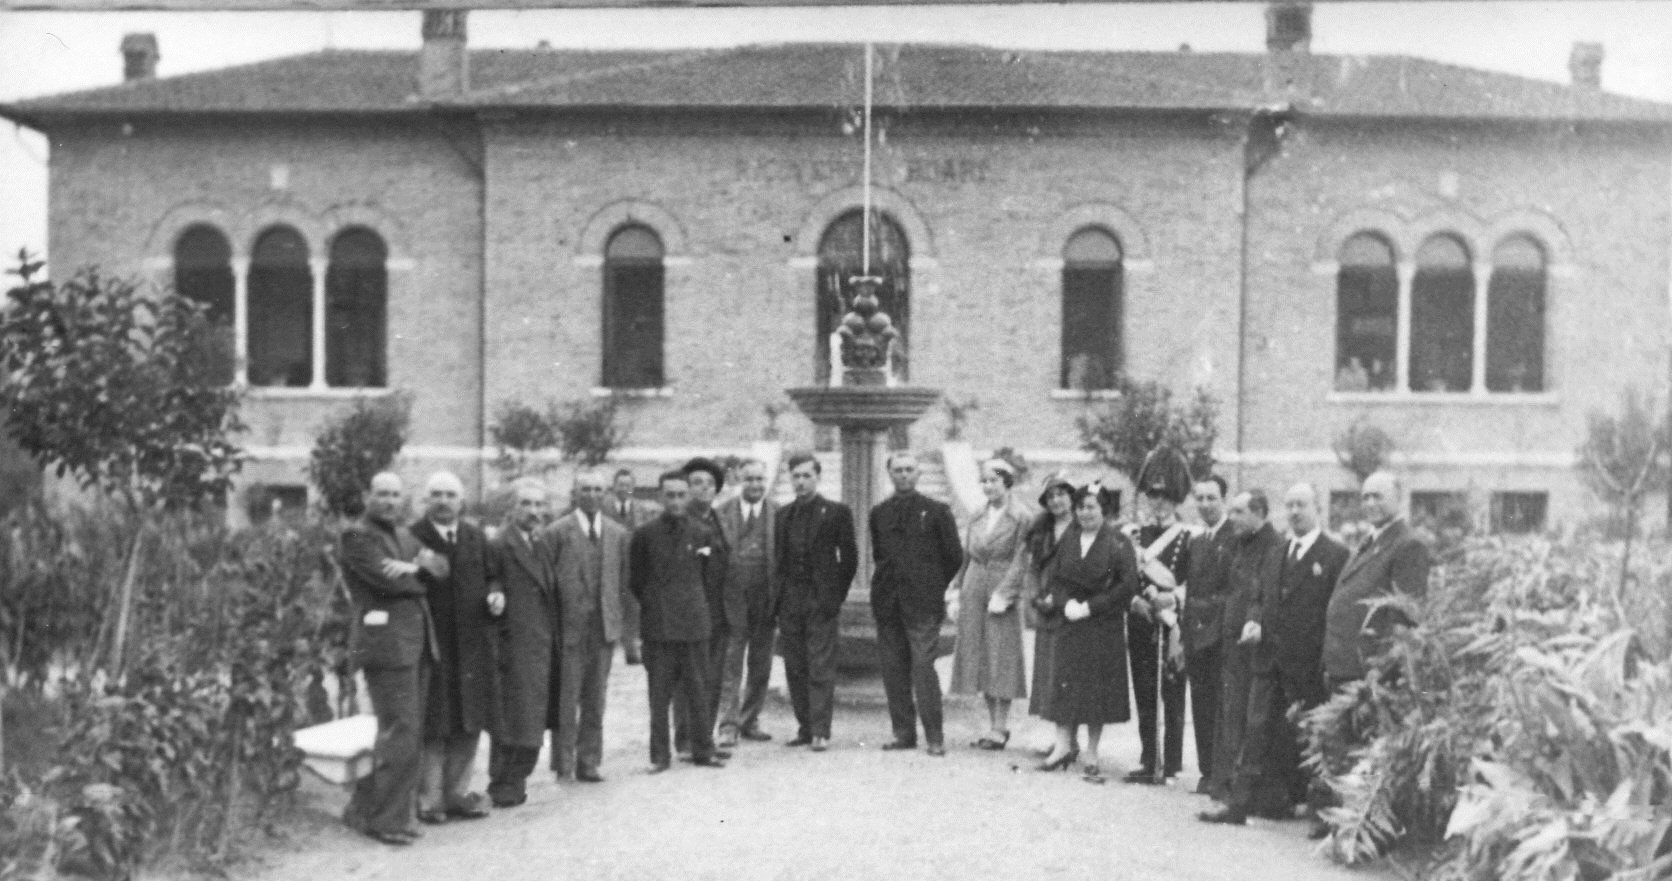
\includegraphics[width=\textwidth]{RicoveroBoari}
    \caption*{Il ricovero \index[Luoghi]{Ricovero A. Boari}\textbf{A. Boari} in via \index[Luoghi]{Reale (via)}Reale, vicino all'Ospedale, terminato nel 1930. Tra le persone presenti nella foto si riconoscono  \index[Personaggi]{Meruzzi dott. Cassiano}Meruzzi Cassiano, il secondo da sinistra a fianco a \index[Personaggi]{Tazzari Luciano (fotografo)}Luciano Tazzari e \index[Personaggi]{Marini Giuseppe}Marini Giuseppe è il primo da destra.\label{fig:RicoveroBoari}}
    %\vspace{-0.3cm}
\end{figure}

\newpage

 \begin{figure}[htb]
    \centering
    %\vspace{-0.7cm}
    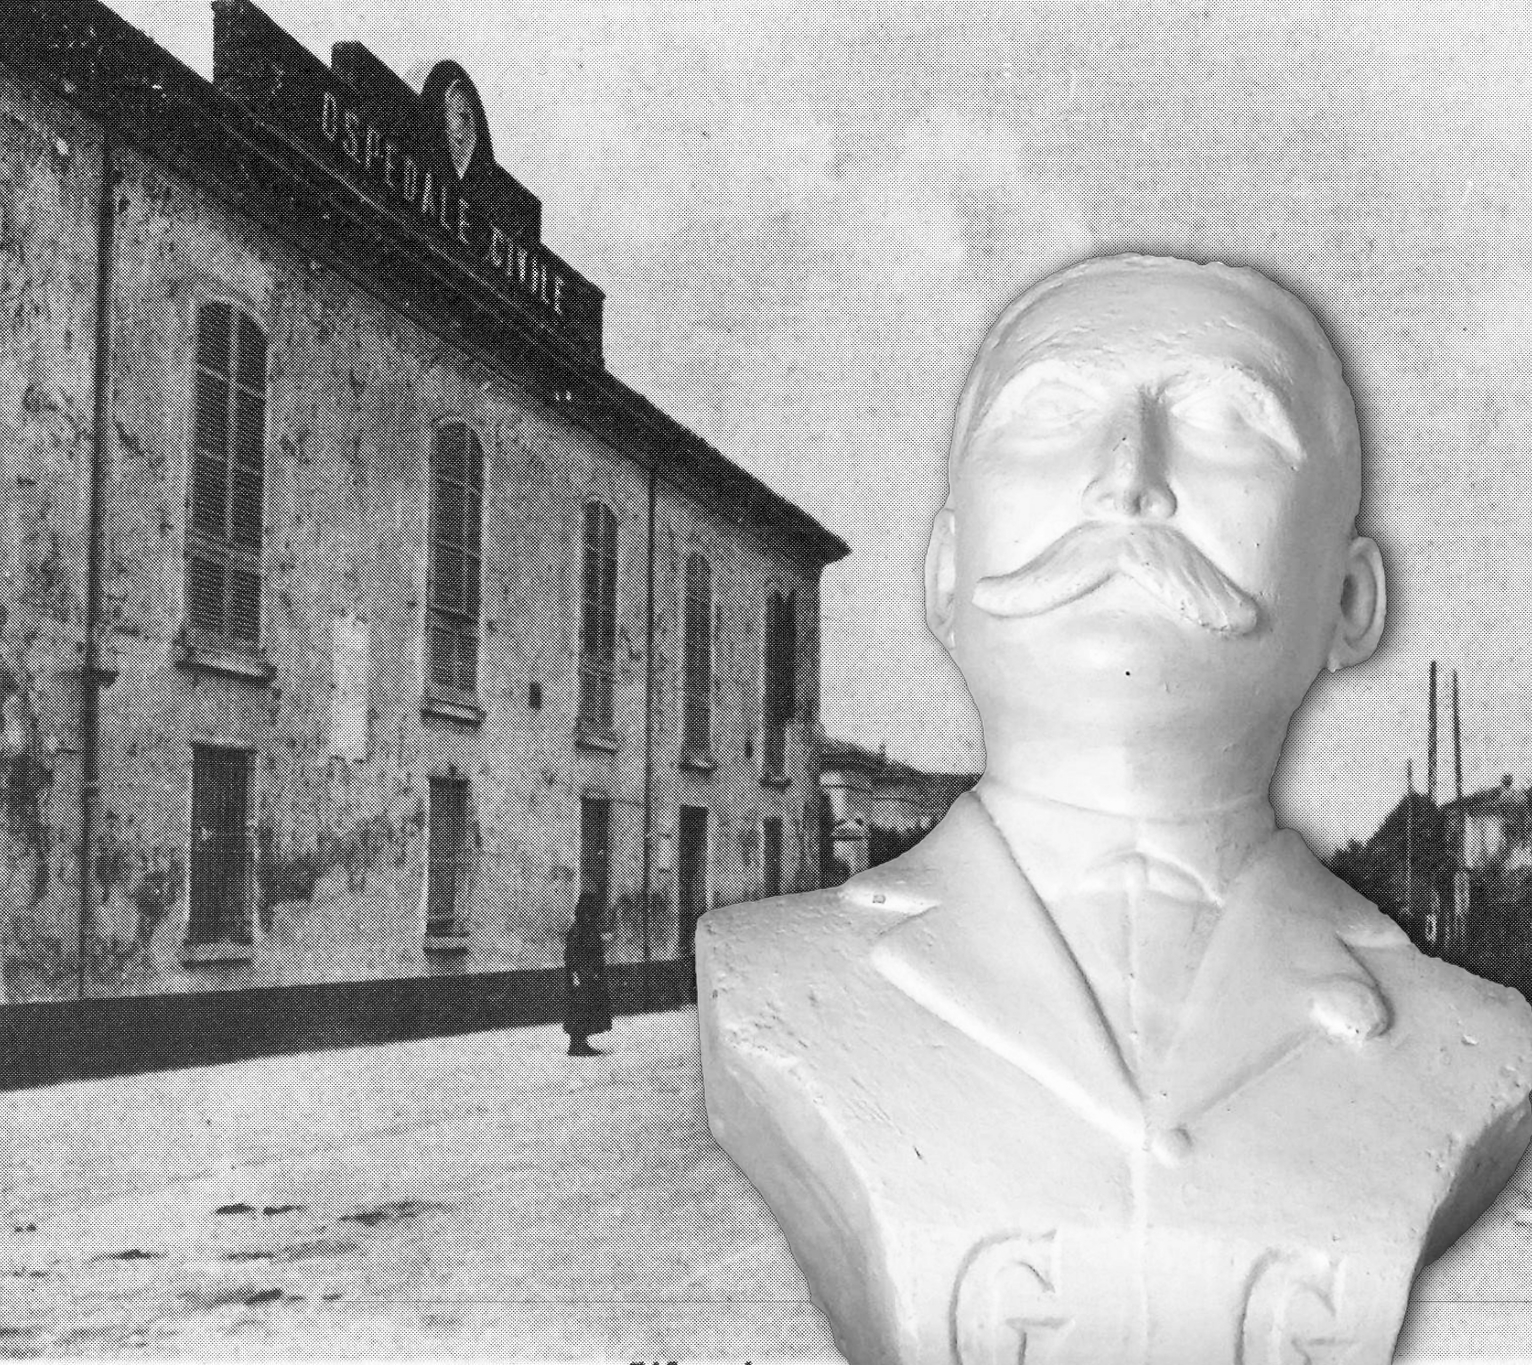
\includegraphics[width=\textwidth]{ospedale}
    \caption*{\label{fig:gamberini}Il busto del Dr. \textbf{Giulio Gamberini}\index[Personaggi]{Gamberini Dr. Giulio} e l'omonimo ospedale.\index[Luoghi]{Ospedale G. Gamberini di Alfonsine}}
    %\vspace{-0.3cm}
\end{figure}


%-------------------------------------------------------------------------------
%	CAPITOLO 28
%-------------------------------------------------------------------------------

\chapter{Uno stronzo nella pentola}
Il signor \index[Personaggi]{Camerani Matteo (farmacista)}Matteo C.\:.\:.\footnote{\textbf{Matteo Camerani} fu un farmacista e fu figlio di  \index[Personaggi]{Camerani dott. Giannantonio (governatore)}Giannantonio Camerani, avvocato, governatore e Giudice di Pace, che a sua volta era figlio di \index[Personaggi]{Camerani Matteo (fattore)}Matteo Camerani, fattore della famiglia Spreti che aveva sposato la sorella di \index[Personaggi]{Monti Vincenzo}Vincenzo Monti, \index[Personaggi]{Monti Maria Cristina}Maria Cristina. Può sembrare confusionaria la genealogia ma è di fatto: Matteo (fattore), Giannantonio (governatore), Matteo (farmacista), Giovan Antonio} aveva fatto scodellare la minestra per sé, la moglie, ed i 4 figli e con la moglie cominciarono a soffiare sulle prime cucchiaiate perché si raffreddasse.\\
\indent I ragazzi erano a tavola meno uno, guardavano in giro e non mangiavano.\\
\indent Matteo, visto il posto vuoto: <<Dov'è \index[Personaggi]{Camerani Giovan Antonio}Giov Antonio...?>>\\
\indent I ragazzi zitti e poi: <<Un'iè\footnote{<<Non c'è>>}>>.\\
\indent Matteo\index[Personaggi]{Camerani Matteo (farmacista)}, al servitore: <<Galli val a ciamé, dov'è?\footnote{<<Vai a chiamarlo, dov'è?>>}>>\\
\indent Ragazzi: <<L'è a là fura!\footnote{<<È là fuori!>>}>>\\
\indent Matteo\index[Personaggi]{Camerani Matteo (farmacista)}: <<Perché non mangiate!>>\\
\indent I ragazzi zitti.\\
\indent Matteo\index[Personaggi]{Camerani Matteo (farmacista)}:  <<Magnì... av deg dal scòpul\footnote{<<Mangiate... vi dò delle scopole>> (scapaccioni)}>>.\\
\indent I ragazzi tentano la fuga, ma sono fermati.\\
\indent Matteo\index[Personaggi]{Camerani Matteo (farmacista)}: <<Parchè an magnì?\footnote{<<Perché non mangiate?>>}>>\\

\indent I ragazzi timidamente: <<Parchè Vàn Antoni\index[Personaggi]{Camerani Giovan Antonio}... la mès un strònz in t'la pignata\footnote{<<Perché Giov Antonio ha messo uno stronzo nella pentola>>}>>.\\
\indent Matteo: <<Ahc! Vigliac!\footnote{<<Bleah! Vigliacco!>>}>> e buttò tutto all'aria.\\
\\
\centerline{\rule{1.5cm}{0.4pt}}\\
\\
\index[Personaggi]{Boari Attilio (farmacista)}Boari era farmacista col signor Matteo\index[Personaggi]{Camerani Matteo (farmacista)}. La mattina del sopracitato fatto, non si sentiva bene.\\
\indent Per rinforzarlo sulle 11 gli portarono una tazza di buon brodo... di quello...\\
\indent Torse la bocca e poi: <<Cos'al ste brod. L'ha un fiè!\footnote{<<Cos'ha questo brodo? Fa una certa puzza!>>}>>\\
\indent Ma lo trangugiò egualmente... come ricostituente sostanzioso. I suoi clienti possano ritenersi vendicati... se da lui hanno avuto delle medicine amare!


%-------------------------------------------------------------------------------
%	CAPITOLO 29
%-------------------------------------------------------------------------------
%
\chapter{I maestri di lingua - Araldo il Capolega B...}
\index[Personaggi]{Lanconelli Araldo}Araldo\footnote{\textbf{Araldo Lanconelli}, (ndr) tutto ciò che so di lui è che sua figlia si chiamava Angelina e che questa fu presente al matrimonio di \index[Personaggi]{Marini Marino}Marino Marini. Tuttavia, Mingazzi ci suggerisce che Araldo coprì la carica di assessore.}, seduto, calvo, con la coppole sulla cervice, ben nutrito, baffi, spioventi, alla moda, era un bell'uomo. Dritto non ci stava perché era zoppo... e così nelle concioni\footnote{Discorsi} dei repubblicani, si vestiva di nero e si metteva in evidenza nel palco accanto a \index[Personaggi]{Mirabelli Roberto (onorevole)}Mirabelli\footnote{\textbf{Roberto Mirabelli}, onorevole, di origine calabrese, più volte deputato di Ravenna per il PRI} o \index[Personaggi]{Mazzolani Ulderico (onorevole)}Mazzolani\footnote{\textbf{Ulderico Mazzolani}, onorevole repubblicano}, essendo un bel pezzo... decorativo.\\
\indent Con le sue idee repubblicane non transigeva, era attaccato alla carica e fu anche assessore.\\
\indent Una sera, durante l'assessorato, si recò a casa, come d'abitudine all'ora di cena, del \index[Personaggi]{Meruzzi dott. Cassiano}Dr. Meruzzi\footnote{Dr. \textbf{Cassiano Meruzzi}, medico condotto di Alfonsine, cugino di Cassiano Bagnara, figlio di Giovanni, proprietario della casa di Vincenzo Monti.}. Poveretto non stava più nella pelle, rideva, si contorceva, faceva delle smorfie.\\
\indent Allora cominciò questo dialogo:\\
\indent Dr. Meruzzi\index[Personaggi]{Meruzzi dott. Cassiano}: <<Insomma, sei troppo contento... hai qualche cosa, dillo.>>\\
\indent \index[Personaggi]{Lanconelli Araldo}Araldo: <<Ecco. Noi repubblicani, a fasèn un oratorio a què drì a la mura d'Terulin\footnote{<<Noi repubblicani facciamo un oratorio qua dietro le mura di Terulin>> - (ndr) non ho trovato corrispondenze con `Berulin'}>>.\\
\indent Donne di casa: <<Oh! Bene così andiamo a pregare... è vicino.>>\\
\indent \index[Personaggi]{Lanconelli Araldo}Araldo si rabbuia e tace.\\ 
\indent \index[Personaggi]{Meruzzi dott. Cassiano}Dr. Meruzzi: <<Voi repubblicani, mangia preti, non ci sarebbe altro... che faceste proprio una chiesa.>>
\indent \index[Personaggi]{Lanconelli Araldo}Araldo in fretta: <<Ma che cisa, a fasèn un pisadur!\footnote{<<Ma che chiesa, facciamo un pisciatoio!>>}>>.\\
\indent \index[Personaggi]{Meruzzi dott. Cassiano}Meruzzi e donne risposero con una risata e poi <<Puh!>>\\
\indent \index[Personaggi]{Meruzzi dott. Cassiano}Meruzzi: <<Alora té da dì un orinatoio...\footnote{<<Allora devi dire orinatoio>>}>>\\
\indent \index[Personaggi]{Lanconelli Araldo}Araldo: <<L'è l'istes, l'è question d'paròl\footnote{<<È lo stesso è questione di parole>>}>>\\
\indent Era anche assessore alla pubblica istruzione certamente se ne intendeva molto e poteva dire anche altro.

Un altro giorno il nostro \index[Personaggi]{Lanconelli Araldo}Araldo, raccontava: <<L'ha scrèt a cà \index[Personaggi]{Forlivesi Sebastiano `Nisò d'Furlivési' (commerciante)}Nisò d'Furlivési\footnote{\textbf{Forlivesi Sebastiano}, nato nel 1830 e morto nel 1905, è il primo dei quattro alfonsinesi che in un modo o nell'altro furono coinvolti nelle varie imprese garibaldine. Partecipò fin dall'inizio alla difesa della Repubblica Romana (1849). Con l'unità d'Italia ebbe a ricompensa della sua attività garibaldina il permesso di aprire una bottega. Quella bottega, passando di figlio in figlio, è ancora oggi attiva in Corso Garibaldi ed è sempre stata chiamata "Butega dla Formazala".} cl'à sintì \index[Personaggi]{De Maria Ugo (professore)}Ugo d'De Maria\footnote{\textbf{Ugo De Maria}, libero docente dell'Università di Parlemo. Fu allievo del Carducci.} in piaza a Palermo, che siringava la folla, contra a Nasi\footnote{<<Ha scritto a casa Nisò d'Forlivesi che ha sentito Ugo De Maria in piazza a Palermo che siringava (per arringava) la folla>>}>> (era il tempo dello scandalo Nasi\footnote{Il Ministro della Pubblica Istruzione, Nunzio Nasi venne accusato di gravi irregolarità nel suo operato. Si parla di corruzione, sussidi ingiustificati, firme sospette, favoritismi, spese personali pagate con i soldi pubblici.})\\
\indent Speriamo che il buon Dio tenga lontano ai palermitani il mal d'urina! Ce ne sarebbero troppe, ma finiamo con l'ultima.\\

\vspace{0.5cm}
\centerline{\rule{1.5cm}{0.4pt}}
\vspace{0.5cm}

Un giorno, al nostro Araldo viene consegnata la scheda per il censimento della popolazione. Da letterato si mette subito all'opera.\\

\newpage

\textcal \Huge
Araldo L\:.\:.\:.\: fu \:.\:.\:.\:\\
\normalfont \normalsize
di professione:
\textcal \Huge Agente Urale
\normalfont \normalsize (per `rurale')\\
di religione: 
\textcal \Huge Ateo

\normalfont \normalsize

\indent Speriamo bene che il nostro protagonista non vada alla storia... e che la scheda di suo pugno non vada in bella mostra... in vetrina.\\

\vspace{0.5cm}
\centerline{\rule{1.5cm}{0.4pt}}
\vspace{0.5cm}


Nel momento rosso i socialisti avevano caricato un buon uomo di molte frasi, capite come poteva e secondo lui solo\footnote{Interpretate a modo suo}.\\
\indent Necessitava una concione\footnote{Discorso solenne in pubblico}.\\
\indent Il nostro uomo, rosso, forte, gesticolante cominciava.\\
\indent <<Soci, amici, compagni, sucilèsta, d'la sucietè, d'la fratelênza, d'la adunênza, d'la cumbrècula, d'la sozia di cuntadèn.\footnote{<<Soci, amici, compagni, socialisti, della società, della fratellanza, dell'adunanza, della combriccola, della socia dei contadini>>}>> Punto e basta il repertorio era esaurito con un <<Evviva noi!>>\\
\indent Per sentire questo discorso migravano molte staffette, parecchi giorni prima; ed il giorno  dell'adunanza i contadini irreggimentati.\footnote{Si muovevano in molti per ascoltare ed il giorno dell'adunanza era tutti inquadrati e pronti all'ascolto} \\
\indent Si vede che mancavano persone a conteggiare quante suole delle scarpe... costava la concione.

 \begin{figure}[htb]
    \centering
    %\vspace{-0.7cm}
    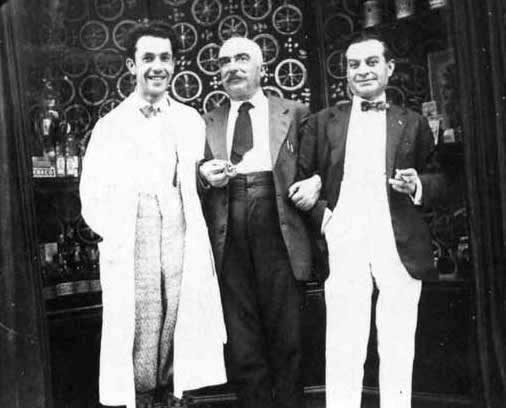
\includegraphics[width=\textwidth]{meruzzi}
    \caption*{I farmacisti della farmacia comunale di via Mazzini. \\ Partendo da sinistra: Dr. \index[Personaggi]{Stella dott.}Stella, Dr. Cassiano \index[Personaggi]{Meruzzi dott. Cassiano}Meruzzi, Nando \index[Personaggi]{Isani Nando}Isani.\label{fig:meruzzi}}
    %\vspace{-0.3cm}
\end{figure}

%-------------------------------------------------------------------------------
%	CAPITOLO 30
%-------------------------------------------------------------------------------

\chapter{Il fanale ed i bisognosi di un albero}
Col suffragio elettorale allargato e l'aumento della popolazione la legge che pretende di regalare tutto dava al paese 30 consiglieri. Cominciarono le spese per preparare i posti per farli sedere e questo fu il primo danno. Il secondo danno fu lo sciupio di carta, sottratta ai WC per la loro elezione... e così via.\\
\indent La passata amministrazione dei monarchici, aveva fatto collocare un fanale a gasolina presso il \index[Luoghi]{Ponte della Ferrovia}Ponte della Ferrovia per rischiarare il passaggio a livello, l'argine del fiume e la rampa che va al \index[Luoghi]{Borgo Gallina}Borgo Gallina.\\
\indent In una seduta si alza il consigliere S.\: \: del \index[Luoghi]{Borgo Gallina}Borgo Gallina, chiamata ed ottenuta la parola, dice: <<A feg la pruposta d'cavè e lampiòn d'in se pont d'la feroveia, parchè su iè un quelcadun ch'eva bsogn d'andes a tu un élbar in te cant \index[Personaggi]{Alberani Anselmo}d'Albarèn, cui possa andè senza èsar vèst\footnote{<<Faccio la proposta di svellere il fanale sul ponte della ferrovia, perché se qualcuno avesse bisogno d'andarsi a prendere un albero nei campi di Alberani ci possa andare senza essere visto>>}>>.\\
\indent Peccato che non sia stata consacrata a verbale questa genuina proposta!

 \begin{figure}[htb]
    \centering
    %\vspace{-0.7cm}
    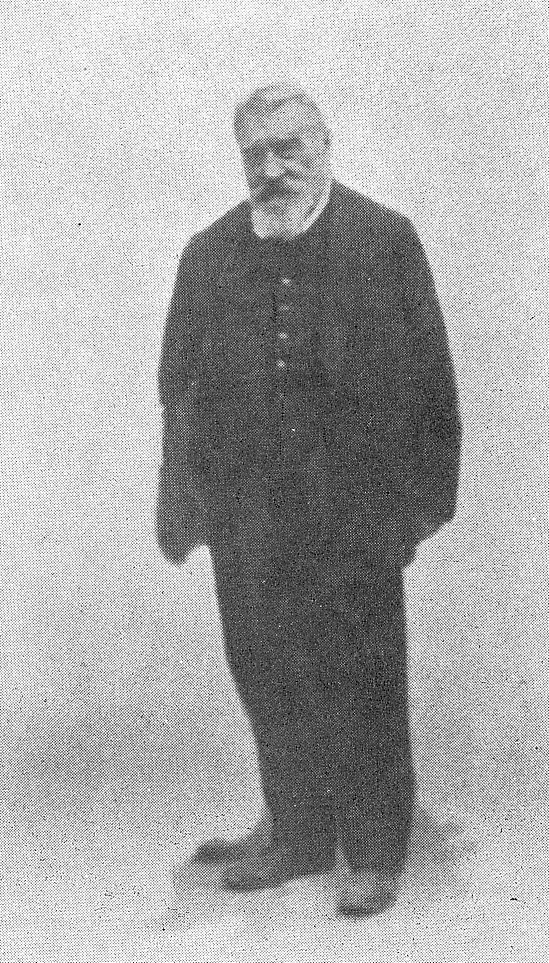
\includegraphics[width=6cm]{alberani}
    \caption[Anselmo Alberani]{\textbf{Anselmo Alberani}\index[Personaggi]{Alberani Anselmo}, uno dei più ricchi proprietari terrieri di Alfonsine, fu pretore. Era il padre di Alberto\index[Personaggi]{Alberani Alberto}, in basso a destra, che fu Sindaco di Alfonsine dal 1922 al 1924.\label{fig:alberani}}
    %\vspace{-0.3cm}
\end{figure}
%-------------------------------------------------------------------------------
%	CAPITOLO 31
%-------------------------------------------------------------------------------

\chapter{In pretura - 12 scudi all'avvocato - Sentenza per donne - Interrogatorio - Un Testimonio - Due asinelli}
\subsection{In pretura}
La pretura, sotto il Papa, era nel \index[Luoghi]{Borghetto}Borghetto, nella casa \index[Luoghi]{Lanconelli (palazzo)}Lanconelli ora \index[Luoghi]{Martini (palazzo)}Martini e precisamente sopra lo spaccio. Nello spaccio e camera retrostante vi erano le prigioni.\\
\indent L'attuale camera dello spaccio era la prigione, larga, dove i prigionieri attraverso la finestra dell'orto, parlavano liberamente col pubblico, chiedevano la carità, mettevano fuori una sporta che i passanti riempivano di cibi.

\subsection{12 scudi all'avvocato}
L'avvocato \index[Personaggi]{Baldrati Girolamino (avvocato)}Girolamino Baldrati, della famiglia ancora esistente dei Cavaler, aveva la fama di tirar fuori i prigionieri, ed a lui affluivano i clienti. \\
\indent Un giorno, parlava attraverso la finestra con un contadino d'Umana, carcerato e suo cliente, al quale esponeva le difficoltà di tirarlo fuori, poi concluse: <<Ti garantisco di tirarti fuori, ma ho delle spese, bisogna che tu mi dia dodici scudi.>>\\
\indent Il contadino dopo i soliti stiracchiamenti contrattuali dovè chinare la testa e promettere all'avvocato di fargli tenere anticipati i chiesti dodici scudi.\\
\indent Tra la finestra superiore socchiusa, vi era il pretore a prendere il fresco, e ad ascoltare il colloquio.\\
\indent Partito che fu l'avvocato, questo pretore certo \index[Personaggi]{Amar\:.\:. d'Ferrara (pretore)}Amar\:.\:. d'Ferrara di famiglia illustre, chiamò \index[Personaggi]{Fantini}Fantini, custore delle carceri e gli ordinò di portargli su il contadino carcerato al quale disse: <<Sono io e non l'avvocato che ti deve liberare. Se mi dai i dodici scudi ti mando a casa subito, se no ti tengo dentro un pezzo.>>\\
\indent Il contadino: <<Propi am manda a ca?\footnote{<<Mi manda proprio a casa?>>}>>\\
\indent Pretore: <<Si, se mi dai i dodici scudi.>>\\
\indent Contadino: <<Alora a mend a dì a mi fradel cu mi purta\footnote{<<Allora mando a dire a mio fratello che me li porti>>}.>>\\
\indent Fu rimesso in carcere... in attesa. Intanto l'avvocato \index[Personaggi]{Baldrati Girolamino (avvocato)}Girolamino, non vedendo i dodici scudi andò alla solita inferiata della prigione, per sollecitarli dal cliente.\\
\indent Là seppe che il suo cliente era stato liberato senza processo e che i dodici scudi li aveva avuti il pretore... che finì col litigare con l'avvocato.

\subsection{Sentenza per donne}
Tre gentildonne dei \index[Luoghi]{Borgo Sabbioni}Sabbioni\footnote{Il \textbf{Borgo dei Sabbioni} era la zona attorno a via Saffi, dove vi era anche la villa della Marchesa, la quale venne sostituita nel dopoguerra da un condominio.} si erano querelate a vicenda innanzi al Pretore \index[Personaggi]{Pompaneri Demenego (pretore)}Pompaneri Demenego, da \index[Luoghi]{Conegliano Veneto}Conegliano Veneto.\\
\indent Questo pretore era un originale, un signore, girava in tuba e code\footnote{Le due code dei vestiti signorili dell'800.} per il paese, proprio quando la massa del popolo portava la `galoza'\footnote{Precisa Mingazzi: "Berretto di canapa/lana, per chi non lo sapesse"}.\\
\indent In udienza, Pretore ad una delle imputate: <<Cosa gasto ti?\footnote{<<Cos'hai fatto te?>>}>>\\
\indent Imputata: <<Mo signor la ma dé dla puténa\footnote{<<Ma signore, mi ha dato della puttana>>}\\
\indent All'altra imputata: <<E ti?\footnote{<<E te?>>}>>.\\
\indent Seconda imputata: <<Me aiò de dla puténa parchè lè steda lì la prèma\footnote{<<Io le ho dato della puttana perché è stata lei la prima a farlo>>}>>.\\
\indent Pretore alla terza imputata: <<E ti?>>\\
\indent Imputata: <<Sgnor che creda cagliè stedi lò dò a dem dla puténa pral premi e me aiò arspost\footnote{Signore creda che sono state le prime a darmi della puttana ed io ho risposto.>>}>>\\
\indent Pretore sentenzia indicando le imputate con un dito: <<Una, due, tre, tre putane fuori dei coioni tutte e tre!>>

\subsection{Un testimonio}
L'abate \index[Personaggi]{F\:.\:.\:. (abate)}F\:.\:.\:. aveva sparato collo schioppo contro il fiume ad un passero su di un albero.\\
\indent Per disgrazia andò ad impallinare vari ragazzi che erano a giocare sull'argine del fiume. L'unico testimonio era un povero vecchio, che non capiva troppo bene l'Italiano, non sapeva quel che si dicesse anche per la paura di trovarsi innanzi alla giustizia.	\\
\indent Il Pretore impazientito, al teste\footnote{Testimone}: <<C'eravate voi quanto l'abate ha sparato...>>\\
\indent Teste: <<Sgnor me ai zur che me ai sera, mo \emph{`c'eravate'} an lo visto in villo\footnote{<<Signore le giuro che c'ero, ma `c'eravate' non l'ho visto da nessuna parte>>.}>>.


\subsection{Interrogatorio}
\index[Personaggi]{Mamon}Mamon e \index[Personaggi]{Marturi}Marturi imputati.\\
\indent Pretore a Mamon: <<Che mestiere fate?>>\\
\indent \index[Personaggi]{Mamon}Mamon: <<Sgnor a feg e sansel, e gambarol, e sert, e barbir, e canzuler, e sbrazèt, a tus i chen...\footnote{<<Signore faccio il sensale, il gambarolo, il sarto, il barbiere, il calzolaio, toso i cani>>}>>.\\
\indent Pretore: <<Basta con questi mestieri>> - a Marturi - <<Che mestiere fate?>>\\
\indent \index[Personaggi]{Marturi}Marturi: <<Gnit sgnor\footnote{<<Nulla signore>>}>>.\\
\indent Pretore, brusco: <<Allora siete un vagabondo!>>\\
\indent Marturi: <<Sgnor, cosa vol ca fega e fa ignacosa lò!>> indicando \index[Personaggi]{Mamon}Mamon.\\
\indent Risata generale e la cosa è diventata un proverbio.

\subsection{Due asinelli}
La nostra \index[Luoghi]{Vincenzo Monti (piazza)}piazza\footnote{Piazza Vincenzo Monti} fu costruita nell'orto \index[Luoghi]{Camerani (palazzo)}Camerani\footnote{Nel 1848 come edificio per un nuovo municipio fu deciso l'acquisto della casa Camerani, una vecchia costruzione che si trovava di fronte all'attuale bar di piazza Monti (ex-Tavalazzi) e dell'orto annesso, che dava sulla via chiamata `Violina', perché molto stretta, che dal ponte andava (e va ancora oggi) fino al cosiddetto “Stradone della chiesa” (dal 1882 Corso Garibaldi). L'orto diventò l'attuale piazza, sistemata alla meglio cui fu dato il nome del poeta Vincenzo Monti\index[Personaggi]{Monti Vincenzo} e la Violina fu allargata e selciata con due marciapiedi laterali.}. Nei primordi era pressoché aperta e confinante con l'attigua campagna. Il nostro mercato della domenica, per le merci, e del lunedì, per merci e bestiame, era antico e cominciato fino dal 1700, per età accreditato ed in molto sviluppo quale centro urbano delle molte ville vicine. \\
\indent Mancavano i fabbricati ed in conseguenza i negozi, così che il commercio era disimpegnato dagli ambulanti. I mezzi di comunicazione erano povere strade, non imbrecciate\footnote{Non coperte con brecciame, ovvero pietrisco}, ed ancora più poveri traini, una carretta, con un ronzino, provato alle inginocchiature di S. Antonio\footnote{Provato fino allo stremo}, e sparuti asini. \\
\indent Come al solito i rivenditori legavano gli asini agli alberi della periferia della piazza, in mancanza di stalle o per economia.\\
\indent Un giorno due di questi asini, in fregola\footnote{Stato di eccitazione sessuale degli animali} d'amore si slegarono, fuggirono per la piazza, si fermarono nel maggiore spiazzo, costituito dalla bella mostra delle terraglie\footnote{Vasellame},  ben disposte dai venditori.\\
\indent In questi amori... la giumenta rimase sotto, abbracciata dalle gambe anteriori del maschio che la copriva... e non desistettero dal loro amplesso che a funzioni finite nonostante le randellate loro sferrate sui rispettivi musi.\footnote{Non fermarono l'amplesso se non quando ebbero finito, nonostante le botte sul muso che ricevevano}.\\
\indent Dei piatti... pestati ne rimasero i cocci. Di qui cominciò la lite tra i venditori delle terraglie ed i proprietari degli asini, per i risarcimenti. \\
\indent Il pretore \index[Personaggi]{C\:.\:.\:. (pretore)}C\:.\:.\:. sentenziò: <<Ritenuti i proprietari degli asini responsabili dei danni, doversi il proprietario dell'asino pagare metà dei danni, perché il suo asino aveva pestato e rotto i piatti con sole due zampe, il proprietario della giumenta dovere pagare il doppio del premio, per avere la sua bestia pestato e rotto le terraglie doppiamente con quattro gambe.>>\\
\indent Ai posteri... i commenti.

 \begin{figure}[htb]
    \centering
    \vspace{1cm}
    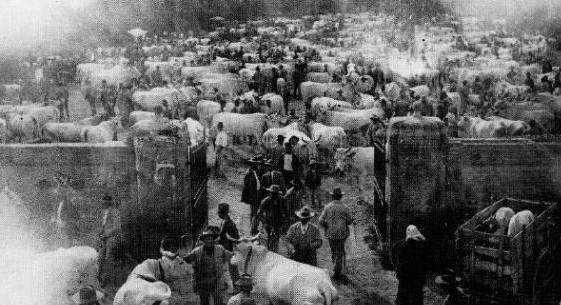
\includegraphics[width=\textwidth]{mercato}
    \caption[Mercato del Bestiame]{Il \textbf{mercato del bestiame}. Nel 1839 fu attrezzata un'area nuova per tale mercato: il \textbf{Campo Boario}\index[Luoghi]{Campo Boario} `e marchè dal besti' in \index[Luoghi]{Corso Garibaldi}Corso Garibaldi, dove ora c'è la ditta Marini con i suoi capannoni\label{fig:mercato}}
    %\vspace{-0.3cm}
\end{figure}











%

%-------------------------------------------------------------------------------
%	CAPITOLO 32
%-------------------------------------------------------------------------------

\chapter{Ho trovato un tesoro}

Eravamo nel periodo, dopo le bande dei ladri. La maggioranza dei ladri erano ancora in galera, ed il popolo fantasticava sulle dicerie che il tale aveva confessato ad un amico di galera di aver seppellito una pentola e marenghi d'oro rubati in qua in là.\\
I luoghi indicati erano la \index[Luoghi]{Chiesa della Madonna del Bosco}chiesa della Madonna dei Boschi, il \index[Luoghi]{Pilastrino della Madonna}Pilastrino della Madonna\footnote{AGGIUNGERE}, ecc... Spesso si vedevano in luogo scavi e tentativi di recupero della gran pentola col tesoro e le fantasie correvano.\\
Una notte il buon \index[Personaggi]{N\:.\:.\:.}N\:.\:.\:. era a letto con la sua \index[Personaggi]{T\:.\:.\:.}T\:.\:.\:. quando lo sveglia un gran pugno tra capo e collo e la voce irata della donna: "Guarda che cos'hai fatto..."\\
\index[Personaggi]{N\:.\:.\:.}N\:.\:.\:. ancora mezzo addormentato e in istato di subcoscenza rispose: "Sta bona la mi \index[Personaggi]{T\:.\:.\:.}T\:.\:.\:. aiò truvé un tesor in te pre dla Madona, e par fei e segn par trovél, aiò c... in sò.\footnote{"Sta buona la mia T\:.\:.\:. ho trovato un tesoro nel prato della Madonna e per fargli un segno e trovarlo vi ho cagato sopra"}"\\
\index[Personaggi]{T\:.\:.\:.}T\:.\:.\:. : "E tesor l'è che tamé c...  in su na gamba e in te let.\footnote{"Il tesoro è che mi hai cagato su di una gamba e nel letto."}"\\
Il resto del risveglio fu molto più reale... perché dovettero alzarsi e preparare il bucato...



%-------------------------------------------------------------------------------
%	CAPITOLO 33
%-------------------------------------------------------------------------------

\chapter{Un tipo originale} 
\index[Personaggi]{M. Giovanni, Giovannone}G. M.\footnote{\textbf{Giovannone M.}, il soprannome è stato definito più sotto} detto S. d' M. era un esperto nel condurre il suo biroccio, nel governo del suo attacco e soprattutto nel vendere il suo vino. \\
\indent Vestiva con un cappello piccolo tondo, alla romagnola, alla cintola aveva la caratteristica fascia rossa dei vetturali\footnote{Incaricato di eseguire un trasporto di merci con un carro, un barroccio o una bestia da soma}, che lo teneva stretto e gli faceva saltar fuori ancor più la pancia.\\
\indent Di mezza età, si era ingrassato, come tutti i corpi sani, guance sporgenti dalle pareti del cranio, un bel parpagliolo rotondo, gli davano una certa rassomiglianza ad una pentola di terracotta.\\
\indent La sua voce da basso profondo era cavernosa, stridula, senza modulazione, tra il toro od il leone infuriato, non rideva mai ed era inclino a prendere tutto sul serio... e parla senza preamboli.\\
\indent Un giorno voleva salire in carrettino, ma si strinse una delle parti genitali, non so come. Qui si era nel tempo del boicott\index[Personaggi]{Faccani Rodolfo (commerciante)}aggio del servizio sanitario, così che il nostro protagonista, consigliato, andò a farsi visitare a \index[Luoghi]{Ravenna}Ravenna dal valente chirurgo prof \index[Personaggi]{Giannetto (professore, chirurgo)}Giannetto e testuamente riferiamo:\\
\indent \index[Personaggi]{C\:.\:.\:.}C\:.\:.\:. (moglie di G.): <<Sgnor professor al se fat mal a un testicul\footnote{<<Signor professore, si è fatto male ad un testicolo>>}>>.\\
\indent G\:.\:.\:.\index[Personaggi]{M. Giovanni, Giovannone} :<<Ignurata... mo che testicolo e mo testicolo, tan si bona dir un `marò'?\footnote{"Ignorante... ma che testicolo e testicolo, non sei capace di dire un marone?"}\\
\indent Il professore rise ed esaminò il paziente e si pronunziò: <<Qui bisogna asportare il testicolo malato.>>\\
\indent \index[Personaggi]{M. Giovanni, Giovannone}G\:.\:.\:. : <<Maiun, mo el pu bon?\footnote{<<Minchioni, ma è però buono?>>}>>\\
\indent \index[Personaggi]{M. Giovanni, Giovannone}G\:.\:.\:. <<Mo si so me sol cun i marò stra a la casa>>\footnote{<<Ma ci sono io coi coglioni tra la cassa>>}\\
\indent \index[Personaggi]{Giannetto (professore, chirurgo)}Giannetto: <<Se non ha stima di me, vada da un altro>>\\
\indent \index[Personaggi]{M. Giovanni, Giovannone}G\:.\:.\:. : <<Quaiù mo sum castra, com'armestia amaséi>>\footnote{<<Coglione ma se mi castra, come rimango accomodato>>}\\
\\
\centerline{\rule{1.5cm}{0.4pt}}
\\\\
Una povera donna un giorno andò dal nostro \index[Personaggi]{M. Giovanni, Giovannone}G\:.\:.\:. che stava terminando il pranzo e gli chiese: <<Allo miga una camera d'afitar?>>\\
\indent \index[Personaggi]{M. Giovanni, Giovannone}G\:.\:.\:. alla moglie \index[Personaggi]{C\:.\:.\:.}C\:.\:.\:. : <<Aièla, faglia avdè.>>\footnote{<<C'è, fagliela vedere.>>}\\
\indent Vista la camera, la povera donna tornò per il responso.\\
\indent Donna: <<Una teraza, una ringhiera...>> (ma non finì)\\
\indent \index[Personaggi]{M. Giovanni, Giovannone}G\:.\:.\:. <<Andì là a si bela>>\footnote{<<Andate là, siete bella>>} scrollò le spalle e la mandò via.\\
\\
\centerline{\rule{1.5cm}{0.4pt}}\\
\\
Aveva un credito con un'oste per una fornitura di vino e non essendo pagato si fece dare un organetto.\\
\indent Successivamente vendette a credito l'organo, a persona che tardava a pagarglielo e trovato in piazza il suo nuovo debitore lo apostrofò:\\
\indent G\:.\:.\:. : <<Ui da cla ca longa, sonal sonal cl'organ?>>\footnote{<<Eih da quella casa lunga (debitore lungo) suona, suona quell'organo?>> - traduzione di Mingazzi riportata fedelmente, probabilmente "debitore lungo" era legato al fatto che questa persona tardasse a pagare il debito.}\\
\\
\centerline{\rule{1.5cm}{0.4pt}}\\
\\
Era un uomo pratico e di buon senso.\\
\indent Un giorno un tale gli disse: <<Voi siete un Signore, perché non andate ad abitare a \index[Luoghi]{Bologna}Bologna e passarvela?>>\\
\indent \index[Personaggi]{M. Giovanni, Giovannone}G\:.\:.\:. : <<A fé chè? Sa steg agl'Infulsen i dis \emph{`S... l'ha di quatrèn'} sa veg a Bulogna i dis \emph{`Chi èl cl'ignurent'}>>\footnote{<<A far che? Se sto ad \index[Luoghi]{Alfonsine}Alfonsine dicono \emph{`Giovannone ha dei quattrini'}, se vado a \index[Luoghi]{Bologna}Bologna dicono \emph{`Chi è quell'ignorante?'}>>}\\
\\
\centerline{\rule{1.5cm}{0.4pt}}\\
\\
Negli ultimi anni aveva dovuto prendere uno scrivano contabile, un simpaticissimo tipo ameno. \\
\indent Un giorno \index[Personaggi]{M. Giovanni, Giovannone}G\:.\:.\:. torna dal mercato e dice: <<Ho comprato un paio di bestie>>\\
\indent Ministro\footnote{Lo scrivano viene chiamato "Ministro" da Mingazzi}: "Dove le avete messe?"\\
\indent \index[Personaggi]{M. Giovanni, Giovannone}G\:.\:.\:. <<Cos'avliv savé vo dgl'intares d'ietar, a mi cuntiv vo i vostar?\footnote{<<Che cosa volete sentire voi gli interessi degli altri, me li raccontate i vostri?>>}>>\\
\indent Un anno dopo i nostri due facevano i conti con un contadino e nella stalla risultava un utile esagerato.\\
\indent Ministro: <<Quelle bestie che compraste quella volta dove le avete messe?>>\\
\indent \index[Personaggi]{M. Giovanni, Giovannone}G\:.\:.\:. : <<A glia avudi stu ca que\footnote{<<Le ha avute costui>>}>> indicando il colono.\\
\indent Ministro: <<È trovato l'errore.>>\\
\indent \index[Personaggi]{M. Giovanni, Giovannone}G\:.\:.\:. <<Vo a scrivì sempar, me a na so cosa ca scriviva s'en avì sgné al besti>>.\footnote{<<Voi scrivete sempre, io non so che cosa scriviate se non avete segnato le bestie>>}\\
Ministro: <<Mo s'an ma dsi, cosa avliv ca seva me>>.\footnote{<<Ma se non me lo dite, che cosa volete che sappia?>>}\\
\indent \index[Personaggi]{M. Giovanni, Giovannone}G\:.\:.\:. <<An la vi da savé vô?\footnote{<<Non lo dovete sapere voi?>>}>>\\
\\
\centerline{\rule{1.5cm}{0.4pt}}\\
\\
Un'altra volta chiamò il ministro e gli disse: <<Scrivì una cartulena a \index[Personaggi]{Pirin Bec}Pirin Bec, a e \index[Luoghi]{Ponte Albergone}Pont Albargon\footnote{<<Scrivete una cartolina a Pirin Bec, a Ponte Albergone>> - Ponte Albergone è la zona e/o il ponte che attraversa il fiume Lamone, con la \index[Luoghi]{Vecchia Albergone (via)}via Vecchia Albergone, sotto \index[Luoghi]{Traversara}Traversara.}>>\\
\indent Il Ministro, inforcata la penna e pronto: <<Come si chiama?>>\\
\indent \index[Personaggi]{M. Giovanni, Giovannone}G\:.\:.\:. : <<Vo scrivì cum cav dec: `a Pirin Bec', in cgnos tot\footnote{<<Voi scrivete come vi dico: `a Pirin Bec', lo conoscono tutti>>}>>\\
\indent Ministro: <<Volete scrivere così, se ne avrà male.>>\\
\indent \index[Personaggi]{M. Giovanni, Giovannone}G\:.\:.\:. : <<Dasim met, scrivì Pirin Bec\footnote{<<Datemi ascolto, scrivete Pirin Bec>>}>>\\
\indent E così fu fatto. E poi \index[Personaggi]{M. Giovanni, Giovannone}G\:.\:.\:. : <<Dsii s'uiè piasù e ven, slin vo dletar. Che zuba se non vien giù il giavolo aveg a la da lò\footnote{<<Chiedetegli se gli è piaciuto il vino e se ne vuole dell'altro. Questo giovedì, se non viene giù il diavolo vado là da lui.>> - `vien giù il diavolo' si dice solitamente riferendosi alle condizioni atmosferiche}>>\\
\indent Ministro: <<Un gni sta più in tla cartulena\footnote{<<Non ci sta più nella cartolina>>}>>\\
\indent \index[Personaggi]{M. Giovanni, Giovannone}G\:.\:.\:. : <<Av si fat da là a mez!\footnote{<<Avete iniziato da lì in mezzo!>> - il ministro aveva cominciato a scrivere da metà cartolina, finendo lo spazio}>>


%-------------------------------------------------------------------------------
%	CAPITOLO 34
%-------------------------------------------------------------------------------

\chapter{Un altro originale - <<Che, che sicurezza la Gigia l'è la mi>>}
Il procaccia postale, prima che la ferrovia fosse attivata nel 1889, andava a prendere e portare tutta la corrispondenza a \index[Luoghi]{Ravenna}Ravenna giornalmente.\\
\indent Col progresso e le strade migliorate, maggior movimento anche il procaccia invece di fare il cammino a piedi, acquistò un ronzino e faceva servizio di trasporto anche per passeggeri, con un cavorino, \textcal{L}\normalfont \:\:\:2\footnote{Un cavorino, detto anche cavurrino, era la carta moneta da lire 2 che portava il ritratto del ministro Camillo Benso Conte di Cavour}, nei primi tempi, 1 scudo (\textcal{L}\normalfont \:\:\:5) negli ultimi, per andata e ritorno. \\
\indent Le tappe erano, partenza dall'osteria in \index[Luoghi]{Vincenzo Monti (piazza)}Piazza\footnote{Piazza Monti}, osteria alle \index[Luoghi]{Glorie}Glorie, Osteria a \index[Luoghi]{Mezzano}Mezzano, osteria della \index[Luoghi]{Camerlona}Camerlona, osteria e stallatico a \index[Luoghi]{Ravenna}Ravenna. Alle osterie tappe vi erano i clienti le commissioni e chi le voleva meglio raccomandare... pagava il quartino di buon vino, al pomeriggio, o l'acquavite alla mattina al procaccia.\\
\indent A \index[Luoghi]{Ravenna}Ravenna bisognava pure ingannare il tempo d'attesa e del riposo del ronzino... ed allora per il procaccia erano altre tappe straordinarie e bevute nelle osterie.\\
\indent Il povero procaccia non si poteva esimere da tante cortesie e libazioni\footnote{Offerta propiziatoria di vino}, il freddo, il caldo, gli facevano venire la necessità di mettere liquido in corpo... e se al ritorno non aveva una sbornia da cataletto.\\
\indent Il vecchio procaccia andò a riposo, ne fu fatto un altro giovane, ispecie perché lo potevano vantare come astemio.\\
\indent Il mestiere però si vede che vuole la sua parte nella manifestazione della vita e così il nostro astemio diventò un forte bevitore e tutte le sere aveva i calori di una solenne sbornia.\\
\indent Venne la ferrovia nel 1889 ed il servizio fu attivato tra la \index[Luoghi]{Vincenzo Monti (piazza)}Piazza e la \index[Luoghi]{Stazione di Alfonsine}Stazione, invece che per \index[Luoghi]{Ravenna}Ravenna, e per quante erano le corse.\\
\indent Le bevute furono maggiori per equipararle alle corse... ed il protagonista era diventato un automa, sempre eccitato, sotto i fumi dell'alcool, irritato, parlava da sé, inveiva ecc.\\
\indent Un giorno lo fermò il Delegato di P. S.\footnote{Delegato di Pubblica Sicurezza} e gli ordinò di portarlo alla \index[Luoghi]{Stazione di Alfonsine}Stazione. Fosse che quel Delegato non lo aveva mai pagato od altro, non ne volle sapere.\\
\indent Allora il Delegato lo apostrofò: "Sono il Delegato di P. S.!"\\
\indent Rispose il procaccia: "Che, che sicurezza, la Gigia\footnote{La sua cavalla} l'è la mi..."\footnote{"Che sicurezza, la Gigia è mia..."} frustò la cavalla e via di corsa, lasciando il Delegato a protestare, ma a piedi.\\
\indent Un'altra volta il nostro originale, aveva consacrato a Bacco forse più del solito, veniva col ronzino e carrettino per la \index[Luoghi]{Strada Sottofiume}Strada Sottofiume\footnote{Attuale via Mazzini}, verso il \index[Luoghi]{Borghetto}Borghetto e sbraitava contro qualche persona.\\
\indent Per una falsa tirata di redini fece montare sull'argine del fiume le due ruote destre del carrettino che si capovolse.\\
\indent Il nostro uomo rimase sotto il carrettino, imprigionato ed incolume, mentre le ruote all'aria seguitavano a roteare; seguitava ad imprecare, come se il caso non lo riguardasse.\\
\indent La Gigia, cavalla, ebbe il buon senso di fermarsi subito...\\
\indent Un'altra volta il nostro uomo doveva firmare la ricevuta dei dispacci nello scompartimento riservato all'ambulante postale, ma si vede che la mano non gli reggeva bene... il capo stazione diede la partenza, ed il treno partì col procaccia... che non volle smontare nelle stazioni intermedie, ma al capolinea di \index[Luoghi]{Ferrara}Ferrara.\\
\indent La Gigia, ed il servizio per il resto della giornata...rimasero sospesi... con delizia dei burloni. \\












































%

%-------------------------------------------------------------------------------
%	CAPITOLO 35
%-------------------------------------------------------------------------------

\chapter{La festa da ballo dei contadini}
I signori del paese erano rimasti in pochi, vecchi e con grattacapi di cambiali in iscadenza, gli artigiani non valeva altro che poco numericamente, e così il carnevale languiva. \\
\indent L'agricoltura faceva progressi, i contadini cominciavano a star bene, alla galozza (berretto giallo di stoppa) cominciavano a sostituire il cappello, erano molli, affiatati, ubbidienti e disciplinati ai loro capi \index[Personaggi]{Sitì}Sitì, \index[Personaggi]{Gallamini Giovanni `Minten'}Minten\footnote{\textbf{Giovanni Gallamini} (22/12/1865 - 20/05/1944)}, \index[Personaggi]{Piteda}Piteda, \index[Personaggi]{Stuanen}Stuanen ecc.\\
\indent In circa un centinaio, per lo più scapoli, si erano uniti in società, pagavano 20 centesimi a testa ogni domenica, per godersi, o faticare per dare una festa da ballo alla sera della domenica grassa. \\
\indent Le adunanze erano molte, per preparare la gran festa, ricordo che una volta ero in casa \index[Personaggi]{Faggioli}Faggioli e tra una Signorina e Sitì si svolse questo colloquio:\\
\indent La signorina, che era in vena di ridere e far ridere: <<Come devono essere vestite le vostre ballerine?>>\\
\indent Sitì: <<Devono essere vestite di bianco, con nastri e sbraciolate fin qui>> e nel dir ciò indicò l'omero del braccio... ed il discorso seguitò col resto degli spropositi e... stuzzicanti domande.\\
\indent Finalmente siamo alla gran sera, gli inviti a stampa ed aggiunte verbali per le belle ragazze e loro madri erano stati fatti. Alla sera alle 19 precise le ballerine dovevano trovarsi tutte accompagnate dalle loro madri all'osteria. Lì le madri levavano fazzoletti, scialle alle loro figlie, che rimanevano coi finissimi vestiti di raso o seta, e venivano consegnati ai complimentari (quelli incaricati delle cerimonie e che le mettevano in ballo poi) irregimentate, ed al braccio ciascuna a un complimentario, al via del capo sala, marciavano in coppie attraverso la piazza, anche se faceva freddo, pioveva ecc. ed entravano in file nel \index[Luoghi]{Teatro Camerani}Teatro Vecchio\footnote{\textbf{Teatro Camerani}, fu costruito probabilmente nei primi dell'800 da \index[Personaggi]{Camerani dott. Giannantonio (governatore)}Giovannantonio Camerani, avvocato e Giudice di Pace, figlio di \index[Personaggi]{Camerani Matteo (fattore)}Matteo Camerani, fattore della famiglia Spreti che aveva sposato la sorella di Vincenzo Monti, \index[Personaggi]{Monti Maria Cristina}Maria Cristina.}, o \index[Luoghi]{Teatro Calderoni, Baraccone}Baraccone\footnote{\textbf{Teatro Calderoni}, detto `e baracò' fu il terzo teatro dell'800 e del '900 alfonsinese. Un possidente terriero e uomo di spicco in paese \index[Personaggi]{Gessi Eugenio (possidente)}Eugenio Gessi, in società con \index[Personaggi]{Santoni Sebastiano}Sebastiano Santoni, decise di costruire un teatro-cinematografo, tra i primi a nascere in Romagna, un primato per Alfonsine. Lo fece costruire tutto in legno da un falegname di nome \index[Personaggi]{Calderoni Antonio (falegname)}Antonio Calderoni, e la gente lo chiamò amichevolmente `e baracò', il baraccone.} dopo, accolte trionfalmente da un ballabile e dai ballerini.\\
\indent Le madri seguivano le figlie col fagotto degli indumenti che andavano a depositare nel camerino delle ragazze. Le ballerine erano subito messe in ballo, e le loro madri in un cantone a fare da spettatrici e commentare...\\
\indent Alla fine di ogni ballo, vi era il "compermesso" cambio dei ballerini. Questi seguivano le ballerine adocchiate durante gli ultimi giri di ogni ballabile con una mano alzata sulla spalla della ballerina, e quando scoccava l'ultima note pronunziavano il sacramentale "compermesso".\\
\indent Con questo sistema il vecchio ballerino si scioglieva dal braccio della ballerina, che dava il braccio al nuovo venuto. Il primo a dire "compermesso" doveva essere il preferito e la ballerina non poteva rifiutare nessuno... essendo ingaggiata per tutta la festa.\\
\indent Una ballerina doveva essere condotta al caffè ogni due balli, massimo e sorbire qualche cosa, per quella che non veniva accompagnata era uno scredito. Uno scredito ancora maggiore per una ballerina era di rimanere per più di due balli con lo stesso ballerino.\\
\indent In questi casi, la società aveva provveduto con la commissione del "tacon" (taccone).\\
\indent Questa commissione era composta di soci che dovevano sorvegliare il cambio regolare di ballerini... ed in caso d'incaglio sostituire i ballerini e scagliare... la ragazza.\\
\indent Questo si diceva fase il "tacon" e succedeva alle brutte... con grave disdoro\footnote{Vergogna} e commenti.\\
\indent Vi era oltre complimentari e quelli della commissione del tacone, il maestro di sala al quale tutti dovevano militarmente ubbidire. \\
\indent Quasi sempre il maestro di sala era il servitore dell'\index[Personaggi]{Monti Cesare (ingegnere)}Ing. Monti\footnote{Ing. \textbf{Monti Cesare}}, un certo \index[Personaggi]{Gallamini Giovanni `Minten'}Minten, un biondo rame, coi capelli tirati sulla fronte, si diceva patina, unti d'olio da sembrare un topo uscito dall'olio, e due baffetti che sembravano stuzzicadenti. \\
\indent Anche questo era un bel tipo e prendeva tutto sul serio cominciando dai suoi strafalcioni.\\
\indent Una notte una maschera, girava con una bandiera, col rischio di spaccare un lume a petrolio. Il nostro \index[Personaggi]{Gallamini Giovanni `Minten'}Minten lo apostrofò: <<Ei mascarotto, tenato su quel bangerotto, che non rompato quel lantarnino>>\footnote{<<Ei mascherotto, tenete su quel bandierotto per non rompere la laterna>>}\\
\indent Nessuno, tranne pochi, rideva a queste scappate, i soci e la massa non aveva allora nozioni della lingua di Dante.\\
\indent A mezzanotte, irregimentate\footnote{Le ballerine}, com'erano venute erano condotte a cena. Qui c'erano cappelletti, lesso arrosto, zuppa inglese per le ballerine ed i soci, e le madri avevano altra cena a parte.\\
\indent Finita la cena, all'una venivano nuovamente irreggimentate le coppie e tornavano alla sala da ballo.\\
\indent Le ore cominciavano a pesare, per smuovere un pò la festa cominciavano le grida, eccole.\\
\indent <<Evviva i soci, Viva le nostre ballerine, Viva noi, Viva la festa, Viva le madri delle ballerine!>>\\
\indent Poi veniva ordinato un ballo per gli invitati, poi un altro per i soci.\\
\indent Guai se le spose tentavano di ballare, era una grossa infrazione, uno scandalo.\\
\indent Quando le ore si facevano più piccine, una voce stonata intonava: <<I invidè s'ia ves dla reputazion is aviareb\footnote{<<Gli invitati se avessero della reputazione se ne andrebbero via>>}>>\\
\indent Ma gli invitati facevano conto di non sentire e la festa continuava fino alle sei. Alle sei tutto finiva con un evviva.\\
\indent I soci avevano faticato, nel dirigere, preparare, spesi tre o quattro scudi a testa per il pranzo, orchestra e festa... e si erano divertiti quando il pubblico diceva <<Oh! Che bella festa!>>.

\begin{figure}[htb]
    \centering
        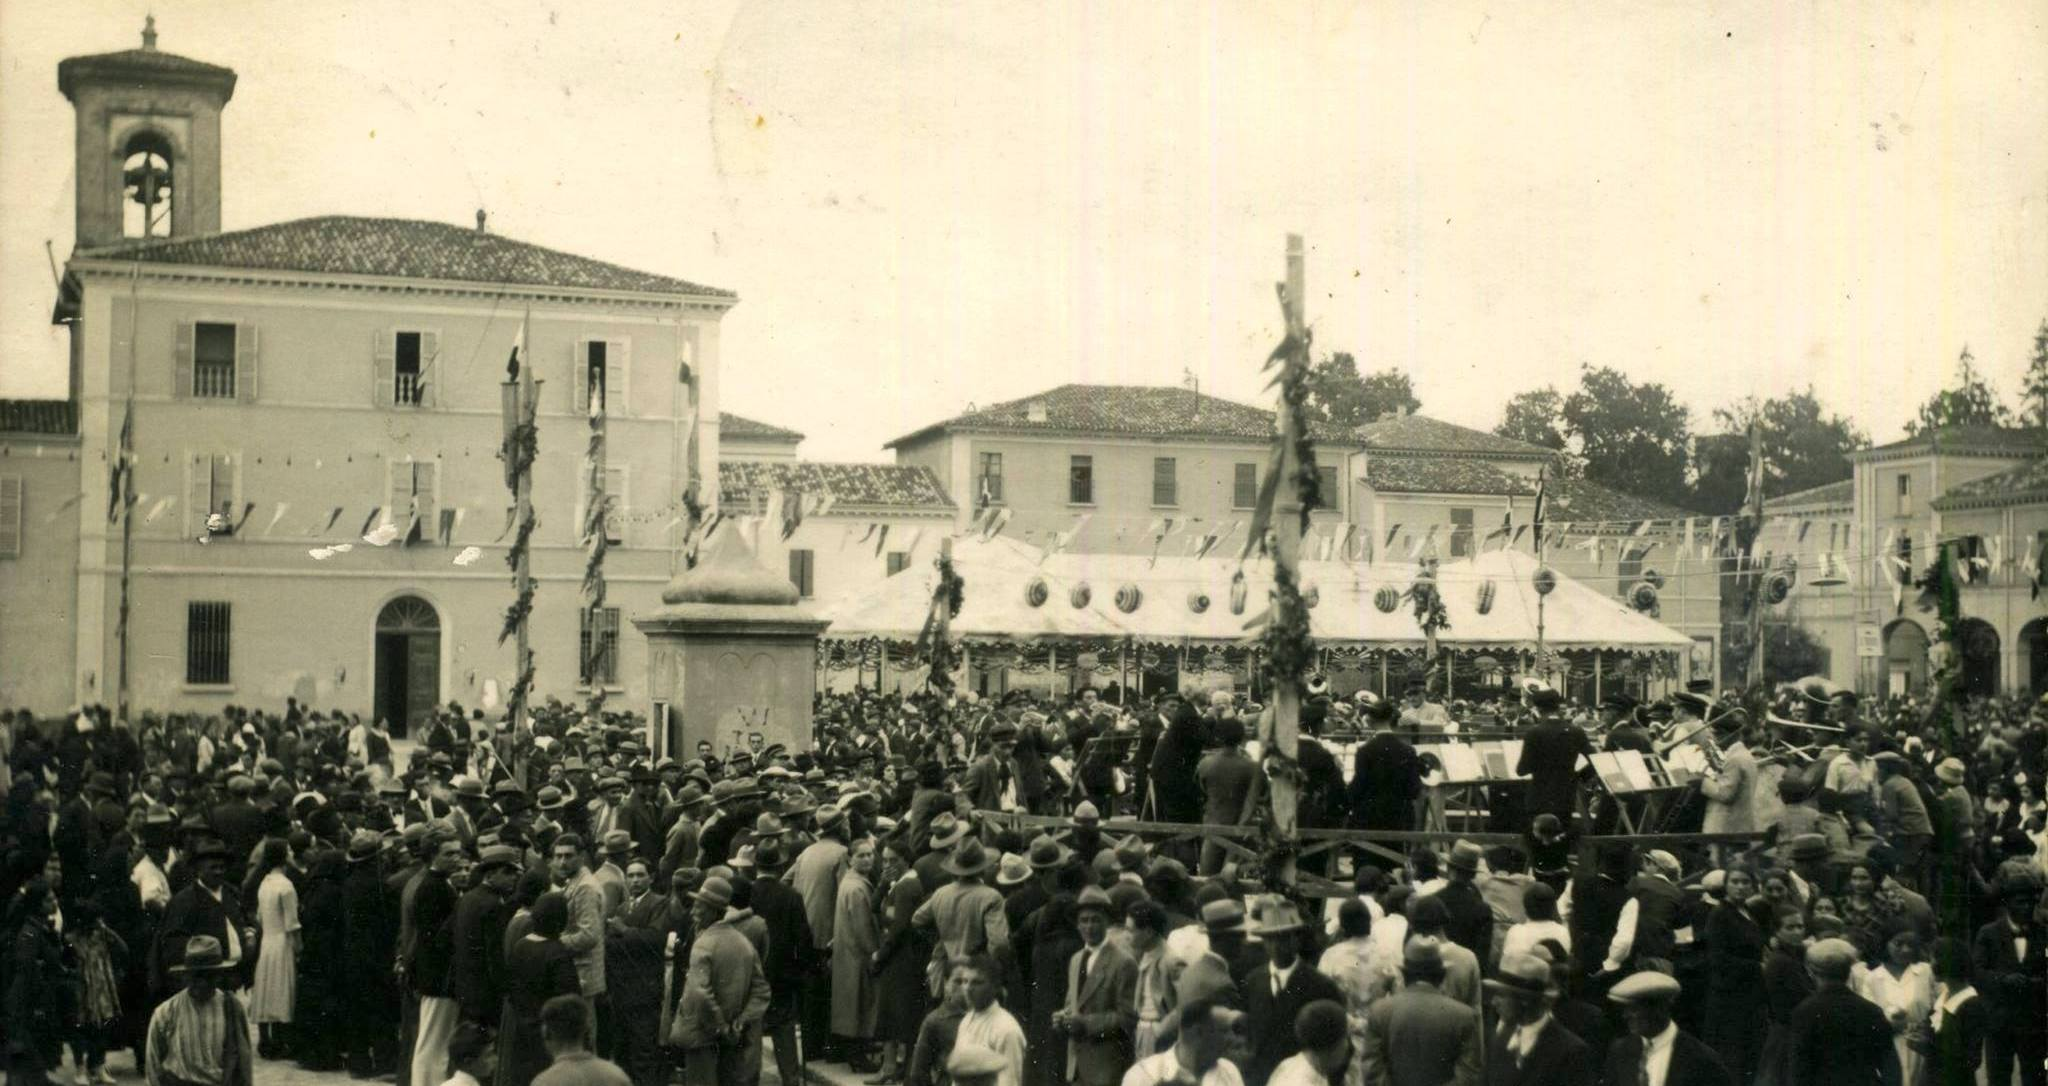
\includegraphics[width=\textwidth]{festa1}
    \vspace{-0.8cm}
\end{figure}

\begin{figure}[htb]
    \centering
    \vspace{-0.45cm}
    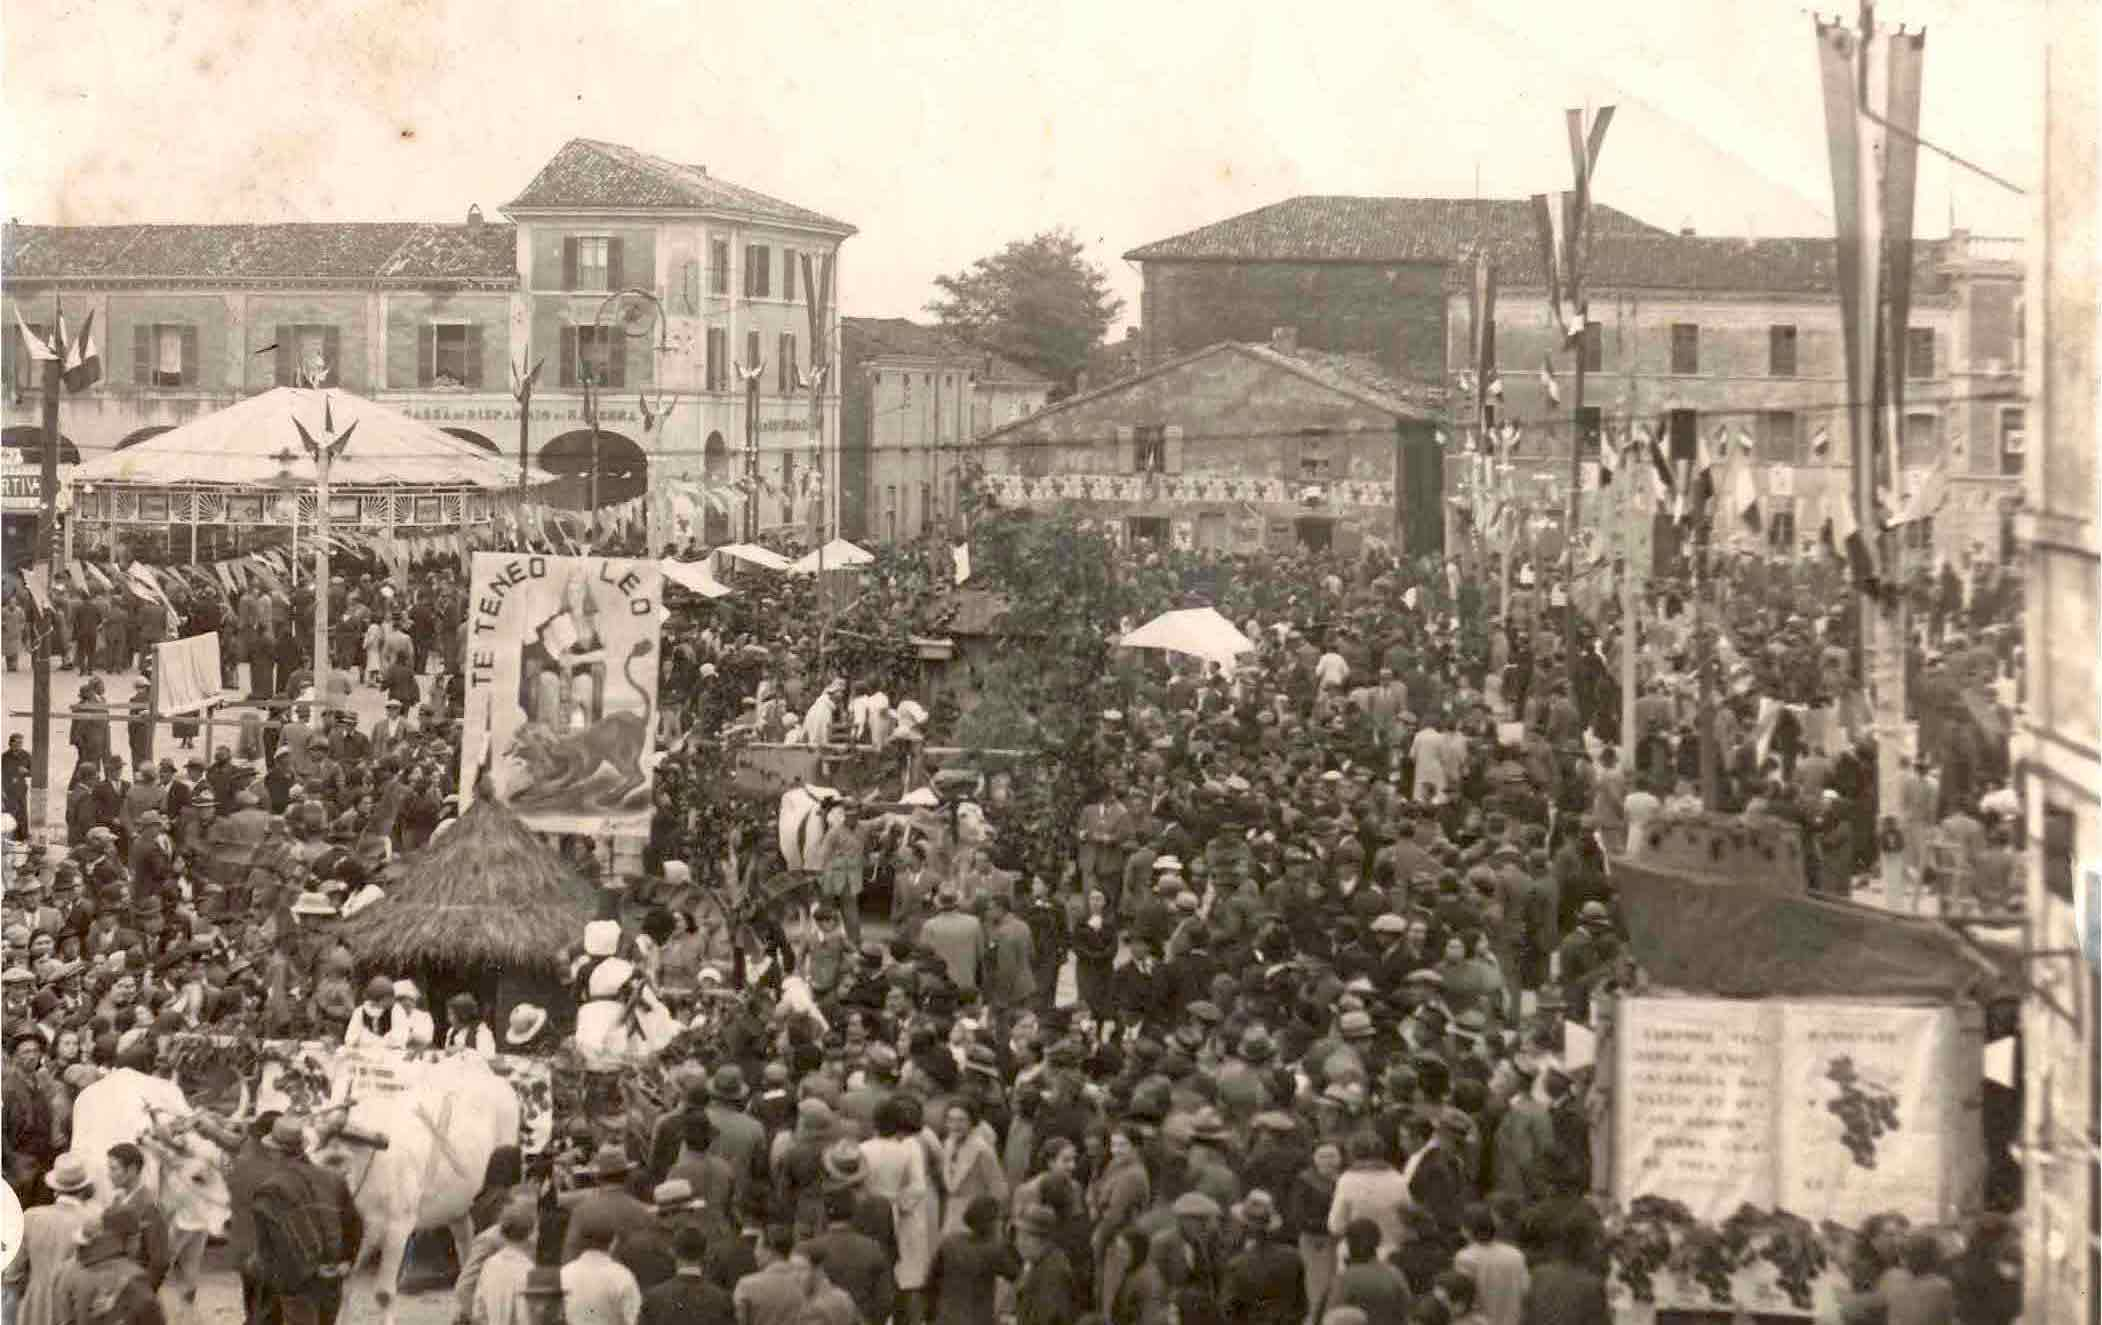
\includegraphics[width=\textwidth]{festa2}
    \caption[Festa dell'uva]{Piazza Monti durante la festa dell'uva 1936. La festa descritta nella storiella probabilmente è la `Festa Gròsa', più antica rispetto alla festa dell'uva. Era chiamata "Fiera di Mezz'Agosto", una vera festa popolare di antica tradizione, ma era già stata dimenticata nel 1929.  \label{fig:festa2}}
    \vspace{-0.8cm}
\end{figure}

%-------------------------------------------------------------------------------
%	CAPITOLO 36
%-------------------------------------------------------------------------------

\chapter{L'atto di divisione tra cognati}
Il notaio \index[Personaggi]{Pirazzoli (notaio)}Pirazzoli si era seduto, lo scrivano \index[Personaggi]{Peppino (scrivano)}Peppino aveva steso la carta bollata sul tavolo, tre cognati e due consorti siedevano intorno al tavolo. \\
\indent Un cognato: <<Alora te t'am dé zeczent frenc...\footnote{<<Allora te mi dai cinquecento lire>>}>>\\
\indent Il secondo cognato: <<No ad deg sol zent scud...>>\footnote{<<No ti dò solo cento scudi>>}\\
\indent Il primo cognato: <<L'è pù l'istes.\footnote{<<È lo stesso" infatti 1 scudo equivaleva a 5 lire}>>\\
\indent Il secondo cognato: <<No a ti darò me e zeczent frenc...\footnote{<<Te li dò io le cinquecento lire...>>}>> tira fuori un lungo stile e si avventa sul primo cognato, che infila la porta e fugge a gambe levate inseguito...\\
\indent Terzo cognato e sorelle: <<Un spò scorrar cun cucalà\footnote{<<Non si può parlare con quello là>>}>>\\
\indent Notaio: <<Me ne vado anch'io finché la strada è libera e buona...>>\\
\index[Personaggi]{Peppino (scrivano)}Peppino, raccolse la carta e l'infilò nella cartella e via... dietro al notaio.\\

\indent Un'altra volta il primo cognato, sempre per questione di somme nelle quali era profondo, aveva disteso, in piazza su di una panca, certi lavori.\\
\indent Un cliente: <<Ti dò una lira e mezzo>>\\
\indent Primo cognato: <<No, a voi trenta bulè\footnote{<<No voglio trenta soldi>> - 1 soldo era equivalente a 5 centesimi di lira, quindi 30 soldi erano esattamente 1 lira e mezzo}>>\\
\indent Cliente: <<T'si mat...\footnote{<<Sei matto...>>}>>\\
\indent Primo cognato credendosi preso in giro: <<A ti darò me la lira e mezzo...\footnote{<<Te la darò io la lira e mezzo...>>}>> e gli si avventò per picchiarlo.\\
\indent È da sperare che questo bravo primo cognato non venga mandato dai sindacati, per turno di lavoro, a prestare la sua opera alla commissione dei cambi con l'estero.\\

\vspace{1cm}
\centerline{\rule{1.5cm}{0.4pt}}
\vspace{1cm}

 \begin{figure}[htb]
    \centering
    %\vspace{-0.7cm}
    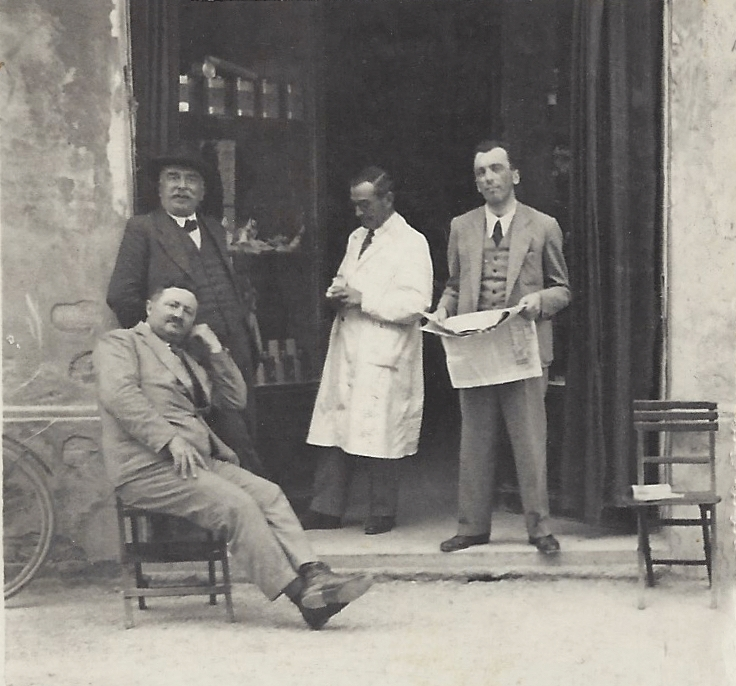
\includegraphics[width=\textwidth]{farmaciamingazzi}
    \caption[Entrata Farmacia con Mingazzi]{L'entrata della farmacia comunale  \index[Luoghi]{Farmacia Comunale} in via Mazzini. Nando \index[Personaggi]{Isani Nando}Isani in camice bianco. Seduto Stefano \index[Personaggi]{Mingazzi Stefano}Mingazzi, dietro il dott. Cassiano \index[Personaggi]{Meruzzi dott. Cassiano}Meruzzi. In piedi col giornale il direttore del Credito Romagnolo Pasi.
	\label{fig:farmaciamingazzi}}
    %\vspace{-0.3cm}
\end{figure}
%-------------------------------------------------------------------------------
%	CAPITOLO 37
%-------------------------------------------------------------------------------

\chapter{Un telegramma}
Il buon \index[Personaggi]{M. P.}P. M. aveva un figlio all'università, con tutte le preoccupazioni della spesa da sostenere e delle bagatelle che esso figlio gli poteva procurare per la sua gioventù e vivacità.\\
\indent Un giorno il signor \index[Personaggi]{M. P.}P.\:.\:.\: si vide recapitare un telegramma, vergato a grossi caratteri dal collettore locale postegrafico \index[Personaggi]{Mercatelli (collettore postale)}Barandellaccio di Mercatelli, così:\\ \textcal \Huge\\
\centerline {Vostro figlio carcerato}\\
\centerline {firmato da persona amica}\\ \normalfont \normalsize \\
\indent Il povero uomo, cominciò a disperarsi, in fretta e furia riempire il portafoglio, perché in qualunque disgrazia bisogna cominciare a vuotarlo... attacca il cavallo e via a \index[Luoghi]{Lugo}Lugo per prendere il treno per \index[Luoghi]{Bologna}Bologna.\\
\indent Il lettore potrà bene immaginare i tristi pensieri che accompagnavano il nostro uomo fino a \index[Luoghi]{Bologna}Bologna... dove arrivò più morto che vivo.\\
\indent Appena arrivato a Bologna, trafilato si recò all'abitazione del figlio e trovata la padrona di casa subito l'apostrofò: <<Mio figlio?>>\\
\indent Padrona: <<È fuori in baldoria con gli amici.>>\\
\indent \index[Personaggi]{M. P.}P.\:.\:.\: : <<Oh, mio signore ma che cos'ha fatto che l'hanno arrestato?>>\\
\indent Padrona: <<Arrestato! Non so nulla. Andiamo a vedere in trattoria.>>\\
\indent In trattoria trovarono un'orgia infernale a banchetto di studenti e non c'era caso né di parlare, né di farsi ascoltare.\\
\indent Con un pò di pazienza trovarono il sospirato figlio... laureato... e la scena cambiò... con una smunta allegra e simpatica al portafoglio di papà.\\
\indent Quel \index[Personaggi]{Mercatelli (collettore postale)}Barandellaccio del telegrafo ne combinava delle curiose!

\vspace{1cm}
\centerline{\rule{1.5cm}{0.4pt}}
\vspace{1cm}

\begin{figure}[htb]
    \centering
    %\vspace{-0.7cm}
    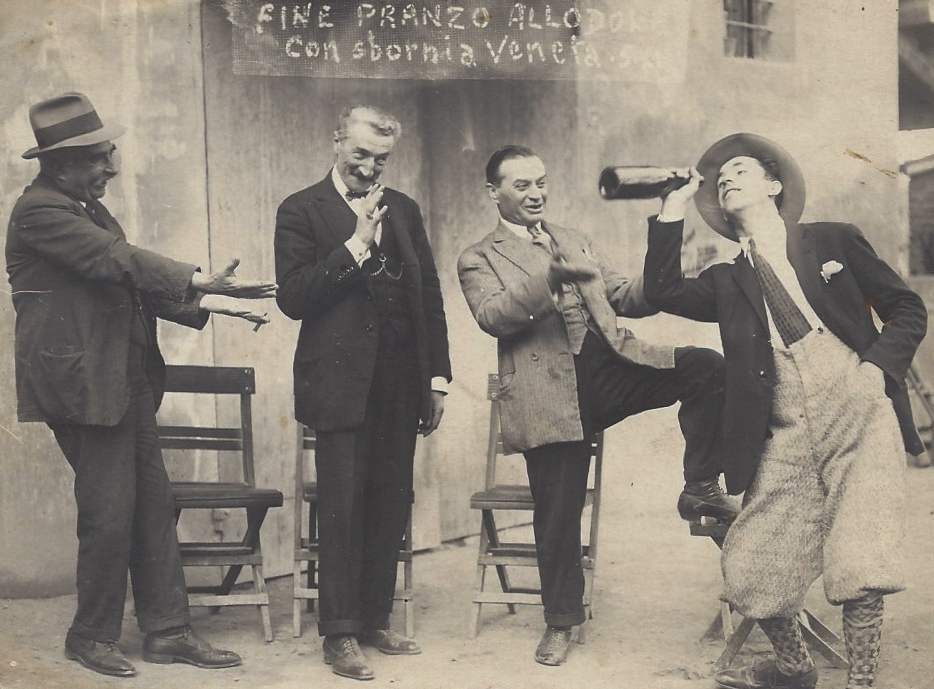
\includegraphics[width=\textwidth]{sbornia}
    \caption[Bevitori - "Sbornia Veneta"]{Una simpatica fotografia trovata nell'archivio di Mingazzi. "Fine Pranzo Allodole - Sbornia Veneta - 5 XI". Da sinistra: Dr.\:Cassiano Meruzzi \index[Personaggi]{Meruzzi dott. Cassiano}, \index[Personaggi]{Tazzari Luciano (fotografo)}Luciano Tazzari (fotografo), Nando Isani\index[Personaggi]{Isani Nando}, Dr.\:Domenico Stella\index[Personaggi]{Stella dott. Domenico}. \label{fig:sbornia}}
    %\vspace{-0.3cm}
\end{figure}
%-------------------------------------------------------------------------------
%	CAPITOLO 38
%-------------------------------------------------------------------------------

\chapter{Un uomo d'affari intraprendente}
Anche questo era un bel tipo. Alto, robusto, dritto, piedi enormi, ginocchie indentro, testa alta, cappello sulla cima della testa, barbuto come un guerriero barbaro. Aveva la mania di essere molto grande, credeva o pretendeva di avere molti appalti di opere pubbliche, corrispondenze ed affari, con anche conquiste femminili e più si scalmanava per ritenersi grande e meno era preso sul serio.\\
\indent Appena si sentiva il treno partire per \index[Luoghi]{Ravenna}Ravenna, sul duro selciato si sentiva un correre e battere forte di tacchi, come un cavallo al trotto.\\
\indent La gente usciva per vedere quel che succedeva... era il nostro bel tipo che ritornava dalla parte della stazione... annunziando a tutti che doveva recarsi a \index[Luoghi]{Ravenna}Ravenna, per grossi affari (che erano bugie) e che aveva perduto la corsa.\\
\indent Tutti ridevano... e facevano finta di compassionare la sua cattiva sfortuna... per farlo parlare dei suoi molti castelli in aria... ingegnosamente architettati.\\
\indent Diceva di spendere quattro mila lire all'anno nella posta, allora che le cartoline postali valevano due soldi, i bolli per le lettere quattro, i telegrammi venti. Non sapeva molto di lettere, non aveva né buste, né carta intestata, non era tanto avanti col progresso... e si crede che per scrivere una cartolina dovesse ricorrere ai suoi figli. \\
\indent Al mattino girava tutta la piazza per mostrare la provvista in una grande sporta... perché si sapesse come se la trattava... e per essere tenuto tra le più ricche famiglie.\\
\indent Apriamo una parentesi per un fatto curioso. \index[Personaggi]{Faccani Rodolfo (collettore postale)}Rodolfo, collettore postale, conosceva la calligrafia di tutti, era scontroso e salace. Un bel giorno il nostro protocollista, innanzi alla posta, aveva cercato di radunare un crocchio di conoscenti e li teneva fermi con chiacchiere, col motivo nascosto di provare loro la sua grande attività affaristica, costrittiva. \\
\indent Rodolfo\index[Personaggi]{Faccani Rodolfo (collettore postale)} esce dalla posta.\\
\indent Il nostro .\:.\:.\: <<Rodolfo, aiel gnint par me?\footnote{<<Rodolfo, c'è niente per me?>>}>>\\
\indent Rodolfo\index[Personaggi]{Faccani Rodolfo (collettore postale)}: <<Uiè cl'la lettra c'av si scret vo ades, aspitì c'av la deg subit...\footnote{<<C'è quella lettera che vi siete scritto voi, aspettate che ve la dò subito...>>}>>\\
\indent Voltò le spalle, entrò nella posta, uscì con la lettera ed al nostro .\:.\:.\: : <<A vò! Lè pu la vostra...>>\\
\indent Il grande affarista rimase muto come un baccalà tra le risate e motteggi\footnote{Punzecchiare con allusioni maliziose} dei presenti.\\
\indent In certa epoca aveva messo gli occhi di triglia, addosso ad una bella contadina bruna, certa \index[Personaggi]{Bice (contadina)}Bice. Non smetteva mai le sue profferte d'amore... e di danaro ed un giorno volle che la bella gli promettesse d'andare con lui a \index[Luoghi]{Ravenna}Ravenna... per consacrarsi all'amore.\\
\indent La bella \index[Personaggi]{Bice (contadina)}Bice, promise ad un fatto, che il suo adoratore doveva ringiovanire col taglio della barba vestito da milord.\\
\indent Così, sbarbato, ben vestito pochi giorni dopo si presenta ansioso alla sua bella, per prendere gli ultimi accordi...\\
\indent La bella \index[Personaggi]{Bice (contadina)}Bice, ridendo, rispose invece molto in disaccordo al suo filarino... precisamente così: <<<Ora senza barba, non vedete come siete brutto... siete più salame di prima>> e l'idillio finì.\\
\indent Sempre in materia di femmine e conquiste al nostro uomo gliene capitò un'altra ancora più bella.\\
\indent Tra le inquiline di una casa che teneva in affitto ce n'era una molto... libera. L'intraprendente nostro uomo si vantava di averla posseduta. La femmina però gliela fece pagare a suon di denaro... mandandolo scornato\footnote{Umiliato, deriso}. Non gli pagò gli otto scudi del fitto. Così il millantatore la citò innanzi al conciliatore, che era il vecchio \index[Personaggi]{Alberani Alberto}Alberani\footnote{\textbf{Alberto Alberani}, sindaco di Alfonsine dal 1922 al 1924.}.\\
\indent Qui riferiamo il colloquio:\\
\indent Conciliatore: <<Tu... hai citato la .\:.\:. perché devi avere otto scudi per il fitto.>>\\
\indent Intraprendente: <<Se>>\\
\indent Conciliatore, alla donna: <<E voi che cosa dovete dire?>>\\
\indent Donna: <<Sgnor, lò -indicando l'intraprendente- e va pu a di cun tot c'um ha .\:.\:. questa che qua un l'à da paghè>>\footnote{<<Signore, lui, va a dire con tutti che mi ha scopato; questa qui la deve pagare!>>}>> con gesto espressivo e forte a palmo aperto sulla parte colpita...\\
\indent L'intraprendente ammutolì.\\
\indent Conciliatore: <<Allora siete pari>> e tra le risate generali dell'uditorio finì la disputa... per la quale è da dire che il nostro grande intraprendete perdè otto scudi, senza nulla avere goduto. 




%-------------------------------------------------------------------------------
%	CAPITOLO 39
%-------------------------------------------------------------------------------

\chapter{I soci, i parenti}
\index[Personaggi]{Graziani, Il Governo (contadino),}Il Governo, un contadino\footnote{Era un contadino soprannominato "Il Governo"}, non quello che comanda, aveva una barca per caccia insieme ad altri due. Non si trovavano d'accordo sulla caccia, a chi la barca? La segarono in pezzi tre.\\
\\
\centerline{\rule{1.5cm}{0.4pt}}\\
\\
Il \index[Personaggi]{Magnanini}Magnanini aveva in parecchi una biroccia, dovevano dividere. Come fare? Segarono le stanghe, il letto, e dei gavoli delle ruote se ne prese uno a te... uno a me... e così alleviarono le loro fatiche da altri trasporti.\\
\\
\centerline{\rule{1.5cm}{0.4pt}}\\
\\
\index[Personaggi]{Cichinoni}Cichinoni... aveva insieme a suo fratello una casa di due stanze, una sopra l'altra nelle \index[Luoghi]{Borse (via)}Borse.\\
Dovevano dividere.\\
Cichinoni voleva quella di sotto, perché la voleva guastare come sua legittima proprietà... sulla quale altro nulla può.


%------------------------------------------------------------------------------
%	CAPITOLO 40
%------------------------------------------------------------------------------

\chapter{Lisco}
Bumb... bumb... bumbum... l'è morto P\:.\:.\:. l'è morto P\:.\:.\:. bum... bum... bumbumb... ecc. col passo secco assordante di due zoccoli ferrati, si sentiva per la via. Era \index[Personaggi]{Lisco}Lisco, che passava a passo veloce per dare al paese un nuovo annunzio funebre.\\
E ciò appena era morto qualc'uno. Come facesse questo disgraziato a conoscere subite tutte le novità e specialmente quelle di morte, nessuno lo sapeva. Forse lo guidava un istinto di godimento per lo spettacolo del funerale nel quale era sempre in testa, specie se vi era la banda.\\
Nella sua idiozia maliziosa si sentiva ammirato e qualche cosa in queste funzioni... di male augurio. Gli annunzi funebri li proclamava coi panni da fatica, zoccoli, saccona, calzoni rimboccati, cappello rovesciato e fissato in testa sul tondello copri testa. Ai funerali precedeva tutti... al rombo della sera musica... e canto... sbirciando di traverso gli spettatori fermi sui marciapiedi. Lo seguiva uno stuolo di bambini.\\
Questo disgraziato, idiota, seguendo un funerale credeva d'andare alla festa... sfoggiando il vestito nuovo, con sul panciotto una catenella da sembrare il barbazzale\footnote{Catenella che unisce i due occhi del morso passando dietro la barbozza del cavallo} di un cavallo focoso.\\
Il suo linguaggio era tutto speciale: "siglio" per \emph{si}, "miglio" per \emph{me}, "iglei" per \emph{lei}, ecc. Non sapeva né il dialetto né l'italiano,,, che credeva d'inventare. Le comitive allegre lo fermavano e per l'esca di qualche soldo lo facevano dire il dizionario dei suoi sproloqui e ridevano.\\
Oltre che l'uomo del male augurio per gli annunzi funebri si era anche arrogato la specialità degli auguri di capo d'anno ed il suo da fare per questa impresa durava vari giorni.\\
Chi voleva ridere rispondeva al buon anno di \index[Personaggi]{Lisco}Lisco "grazie, altrettanto" ma \index[Personaggi]{Lisco}Lisco... subito: "datemi due soldi" e così passava tutti incassando qualche scudo.\\
Quando si presentò alla rivista militare fu pronto a spogliarsi, ma la commissione lo tenne in disparte per osservarlo meglio e chiesero informazioni al Sindaco presente. Il responso della Commissione di leva fu la classifica di 'idiota'.\\
A chi chiedeva a Lisco, che cosa voleva dire ‘idiota', con serietà rispondeva "vuglio dire miglio sono baibo" (io sono balbuziente).\\
Un giorno, col cappello rovesciato, gli zoccoli nei piedi e nella saccona infilato l'ombrello di tela cerata verde... battendo la sua solita musica, a \index[Luoghi]{Bologna}Bologna andò ad infilare via \index[Luoghi]{Rizzoli (via)}Rizzoli, seguito da uno stuolo di ragazzi che lo motteggiavano. La passeggiata finì, come doveva finire, fu preso dalle guardie e portato a vedere il cielo a scacchi\footnote{Portato in prigione}... per essere rimpatriato. Il bello però venne quando gli sequestrarono 12 scudi, frutto delle guardie. Montò su tutte le furie... ma le guardie sopraffecero e lo immobilizzarono... e lui ad urlare: "Lêdar dasim i mi bulèn!"\footnote{"Ladri datemi i miei soldi!"}\\
La sua deficienza mentale, lo salvò da altre pene... ed a \index[Luoghi]{Bologna}Bologna non andò più.\\

 \begin{figure}[htb]
    \centering
    %\vspace{-0.7cm}
    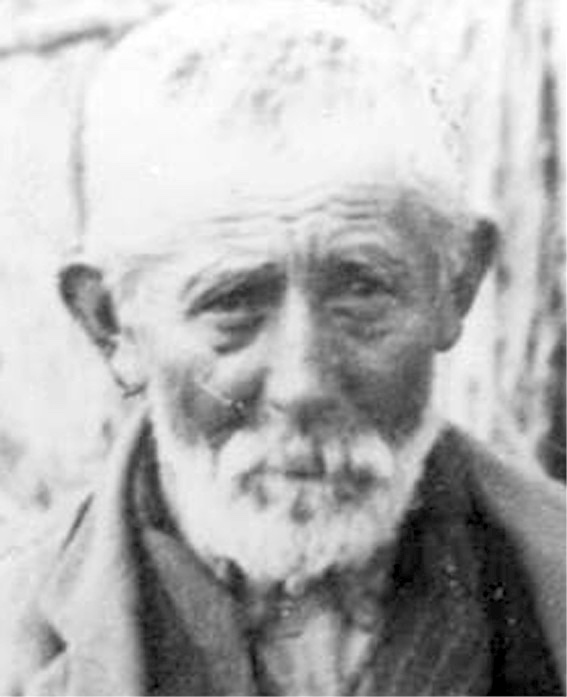
\includegraphics[height=8cm]{Lisco}
    \caption{Lisco, ritratto da vecchio, personaggio famoso ad Alfonsine\label{fig:Lisco}}
    %\vspace{-0.3cm}
\end{figure}




%-------------------------------------------------------------------------------
%	CAPITOLO 41
%-------------------------------------------------------------------------------

\chapter{I due Capelli - Gioti}
\index[Personaggi]{Capelli (avvocato)}Uno affogato nel vino. Parliamo di quello. Era un valore come legale, conscio del suo valore ne era altero e soffriva mal volentieri di fare il suo tirocinio alle dipendenze di un celebre avvocato di \index[Luoghi]{Bologna}Bologna il quale trionfava nei Tribunali con le difese del nostro uomo.\\
\indent L'applicazione allo studio, il mal trattamento od altro rovinarono la salute del nostro emerito avvocato... ed i genitori lo vollero a casa per guadagnare la salute.\\
\indent Qui era medico primario il povero dott. \index[Personaggi]{Gamberini Dr. Giulio}Gamberini, che aveva una grande fiducia nei buoni effetti rigenerativi del vino e cognac.\\
\indent Avendo sotto la sua casa il nostro avvocato, esile, allampanato... senza appetito ed astemio, cominciò a farlo trincare per rinvigorirlo. Fu una sbornia attaccata all'altra e lo rovinò.\\
\indent Solitamente la sbornia di carnevale cominciava in lui a Natale e finiva a Pasqua. Fiutava tabacco e chi lo avesse spolverato ne poteva ammassare qualche ettogrammo\footnote{Il protagonista era talmente impolverato che, scrollandolo, si poteva recuperare qualche ettogrammo di tabacco}.\\
\indent Il povero avvocato era ridotto ad uno stato miserevole dagli aiuti dell'alcool... in mezzo ad una festa da ballo, nella piazza affollata orinava in faccia al pubblico...\\
\indent Se la prendeva coi pretori perché non gli davano la vittoria nelle cause.\\

I suoi ritornelli ed invettive ai principali pretori, chi non li ricorda?
\textcal{	
\begin{center}
\Huge
No, anavoi Capolozzo! Capolozzo!\\
No, anavoi Mambrucon!\:\:\normalfont\normalsize\footnote{<<No, non voglio Capolozzo! Capolozzo; No, non voglio Mambrucone!>>}\footnote{Mambrucone fu pretore ad Alfonsine. Citando Romano Pasi: "Questo pretore Scognamiglio, principe meridionale, soffriva molto il freddo alfonsinese, per cui ascoltava le parti in causa standosene al calduccio del letto, mentre al cancelliere faceva mettere tutto agli atti. Quando la corte si ritirava per deliberare, si tirava la coperta sul capo, e dopo un po', scoprendo il volto, emetteva la sentenza."}
\end{center}}
\index[Personaggi]{Capolozzo}\index[Personaggi]{Mambrucone (pretore)}
\normalfont \normalsize
\noindent Di lui era caratteristica la macchietta.\\
Ecco l'uomo colto... ridotto incolto... dall'alcool.
 \begin{figure}[htb]
    \centering
    %\vspace{-0.7cm}
    
\includegraphics[height=6cm]{Capelli_Avvocato}
    \caption[Capelli (protocollista)]{}
    %\vspace{-0.3cm}
\end{figure}\newpage
\index[Personaggi]{Capelli (protocollista)}

Sotto l'altro\footnote{E ora parliamo dell'altro}. \\Per questo la gola fu fatale. I tortelli hanno ucciso Capelli\footnote{Mia nonna Mariannina Gagliardi, nipote di Mingazzi, si ricorda che spesso Mingazzi raccontava di un certo "Zucò 'd Capèli", il protagonista di questa storiella.}, questa orrenda notizia vi dò!\\
\indent Tipo curioso, si credeva bello, irresistibile alle donne. Permaloso, un pò tardo di comprendonio sotto lo sforzo della digestione.\\
\indent Offriva a tutte le belle ragazze 100 scudi per una gita... con lui a \index[Luoghi]{Ravenna}Ravenna. Distribuiva a 60 anni, alle sue dame il suo ritratto all'età di 20 anni, vestito da sottotenente, nella sua caratteristica figura. La faccia sembrava una gran luna con sopra un guscio d'ovo, che era il berretto, due baffetti spioventi alla cinese, occhini coperti da grosse palpebre, sembrava un maiale della grassa. \\
\indent Si riteneva molto eloquente, faceva il causidico\footnote{Avvocato da poco, di bassa lega.} in pretura ed una volta presentò una comparsa con citazioni latine... che non conosceva. Il Pretore \index[Personaggi]{De Simone (pretore)}De Simone, ebbe a dirgli: <<Ecco spieghi questa...>>\\
\indent Al nostro causidico cadde il mondo addosso e credè rispondere: <<Ecco... si... già... s'intende...>> e fu una risata generale.\\
\indent Aveva lo stipendio da protocollista in comune, ma il suo tempo era diviso per le seguenti funzioni:\\
\begin{itemize}
\item[9.00]purga con acqua - Janos\footnote{Acqua medicinale Hunyadi János, conosciuta e consumata dal 1863, costituita da sale di Glauber e sale inglese.}
\item[10.00]leggere sotto lo scaffale della scrivania il giornale, e brontolare a chi osava varcare la porta del suo ufficio: <<Ho da fare lasciatemi in pace...>>
\item[11.00]entrata nella vecchia latrina del palazzo comunale, dove c'era una gran pietra per posare i piedi, dietro una buca di m. 1,50 per 0,80 e dopo il muro.\\
Giù le brache... chino il corpo in orizzontale, non arrivava ad accovacciarsi sui polpacci... che la scarica avveniva nel muro di contro con una rosa di almeno 60 centimetri. \\
Chi andava dopo di lui vedeva i segni di \index[Personaggi]{Capelli (protocollista)}Capelli.
\item[11.30]Andava alla firma, riceveva 4,5 lettere da protocollare.
\item[12.00] a mangiare.
\item[13.00] a fare il chilo sul sofà e respirare a due riprese, perché troppo pieno.
\item[13.30] per la strada presso le fruttivendole a mangiare arance, mele, mandarini, zucca cotta ecc.
\item[14.00] all'ufficio a cominciare missive d'affari sui grandi fogli da protocollo, poi accartocciava tutto... perché sbagliava perché era troppo pieno... e non concepiva il pensiero.
\item[17.00] (d'inverno) uscito dall'ufficio, passava a rifornirsi di cioccolatini e poi da qualche bella a farseli mangiare.
\item[18.00](se d'estate) all'osteria a ordinare un etto di mortadella, o salame, mezzo litro di vino, e due soldi di pane, con molti bis.
\item[19 - 20] a cena a divorar tutto.
\item[20.30] al caffè cominciava a bere latte mangiar paste, biscotti, pan di Spagna ecc. per qualche mezzo chilo.
\item[21.30] a morosa fino alle 22
\item[22.00] entrato nell'osteria annusava come un cane da trifola, poi chiedeva : <<Che cosa hai rimasto?>>\\
\indent Oste: <<Cappelletti, umido, arrosto, lesso."\\
\indent \index[Personaggi]{Capelli (protocollista)}Capelli: <<Fammi vedere>> poi <<Quanto vuoi per tutto?>>\\
\indent Il contratto era fatto e tutto divorato.
\item[23.00] Chiudevano l'osteria ed il nostro uomo prendeva la via dell'amata... fino all'una.. a fare il chilo e farsi far vento alla pancia perché gli tirava per avere troppo mangiato...
\item[1.00] tornava a casa e dava aria ai polmoni... ed alla strada... per sgonfiare la pancia. Poi a letto fino alle 8.
\end{itemize}

Era assiduo di tutti gli spettacoli ai quali assisteva divorandosi brustole\footnote{Semi di zucca}, caramelle, cioccolatini ecc.\\
\indent Credeva di conquistare le commedianti o cantanti, ronzando sempre loro intorno come un molesto bagarone\footnote{Calabrone}.\\
\indent Una sera il pover'uomo era a godersi uno spettacolo, seduto su una delle prime fila di sinistra del \index[Luoghi]{Teatro Calderoni, Baraccone}Baraccone. Aveva mangiato più del solito, la sua testa era in confusione credendosi ammirato... (e per questo era abile perché aveva una gran cura di mostrare alle artiste il portafoglio e di promettere molto...) ma la digestione lo disturbava molto e lo assopiva. Però non poteva né assopirsi né sedersi comodamente... era come sugli spini per la gonfiezza.\\
\indent Sulla fine di un atto uscì, si appressò alla siepe del \index[Luoghi]{Carraretto Venturi}Carraretto\footnote{Carraretto Venturi, il teatro Baraccone fu spostato nel Carraretto Venturi (e lazarètt) già dal 1894}, ad orinare quando credé di fare uno sforzo per vuotare l'aria... ma il colpo fu tale e forte... da prendere una lombaggine\footnote{Dolore in sede lombare che si acutizza nei movimenti di flessione ed estensione del tronco} (snestar\footnote{Espressione dialettale per `colpo della strega'}) e dovettero portarlo a casa, e chiamato il povero \index[Personaggi]{Novi (dottore)}Dr. Novi e l'infermiere \index[Personaggi]{Domenico Soatti `Mingò d'Galèna` (infermiere)}Mingone di Gallina\footnote{\textbf{Domenico Soatti}, detto Mingò d'Galèna,infermiere.}, che lo sottoposero ad una iniezione calmante.\\

\indent Era sempre tutto gentile... per non far torto al suo budello che tanto lo aiutava. Era geloso di tutti e di tutte.\\
\indent Il povero \index[Personaggi]{Isani Nando}Nando Isani, aiuto farmacista da \index[Personaggi]{Boari Attilio (farmacista)}Boari, quando lo vedeva venire serrava la bussola\footnote{Portantina} della farmacia e si nascondeva nel laboratorio.\\
\indent Cominciava allora la scena da ridere. \index[Personaggi]{Capelli (protocollista)}Capelli, spingeva la bussola, chiamava... strimpellava, perché si metteva in sospetto che nel retro farmacia Nando \index[Personaggi]{Isani Nando (farmacista)} avesse qualche avventura galante... e lui voleva sorprenderlo... per intimare alla femmina... amore anche per lui... \\
\indent La porta rimaneva chiusa e \index[Personaggi]{Capelli (protocollista)}Capelli guardia portone, finché dopo un gran pezzo appariva il povero Nando \index[Personaggi]{Isani Nando (farmacista)} facendo l'imbronciato, e cominciava il dialogo.\\
\indent Capelli: <<Chi avevi...>>\\
\indent Nando: <<Nessuno, che cosa vuol sapere!>>\\
\indent Capelli: <<Va là dimmelo, ti vuoi godere solo tu... ed insisteva per delle ore...>>\\
\indent Capelli a qualche altro: <<Mo chi era la donna, dove è?>>\\
\indent Interrogato: <<Stia zitto è scappata dalla porta di dietro!>>\\
\indent Capelli: <<Porca, non sono capace di trovarla!>>\\
\indent E la commedia si ripeteva spesso... tra le risate.\\

\indent Una delle sue amate stava in \index[Luoghi]{Vincenzo Monti (piazza)}Piazza\footnote{Piazza Monti} di fronte al \index[Luoghi]{Palazzo Comunale}Palazzo Comunale ed aveva le finestre al 2\textsuperscript{o} piano.\\
\indent \index[Personaggi]{Capelli (protocollista)}Capelli si metteva alla finestra del \index[Luoghi]{Palazzo Comunale}Palazzo Comunale, la sua amata... alla sua, distante 150 metri e pretendeva di essere ammirato. Una volta poi avvenne che i saltimbanchi eressero in \index[Luoghi]{Vincenzo Monti (piazza)}Piazza grandi tende ed impedirono l'idillio di ammirazione. Il nostro \index[Personaggi]{Capelli (protocollista)}Capelli se la prese con l'amata... e la piantò per qualche tempo.\\
\indent L'amata però mal soffriva un tale ingiusto trattamento e decise di fermare l'amato bene un sera quando andava a casa. Il colloquio si svolse così:\\
\indent Amata: <<Perché non vieni più?>>\\
\indent Capelli: <<Perché non mi hai guardato dalla finestra...>>\\
\indent Amata: <<Ma come devo fare, ci sono le baracche in mezzo e non si può vedere...>>\\
\indent Capelli: <<A na voi savé me, va dsò da la Pia... (al 3\textsuperscript{o} piano) me a voi t'am guerda\footnote{<<Non lo voglio sapere io, va di sopra dalla Pia, io voglio che tu mi guardi>>}>>.\\

\newpage
Ammiriamo anche noi questo pachiderma.
 \begin{figure}[htb]
    \centering
    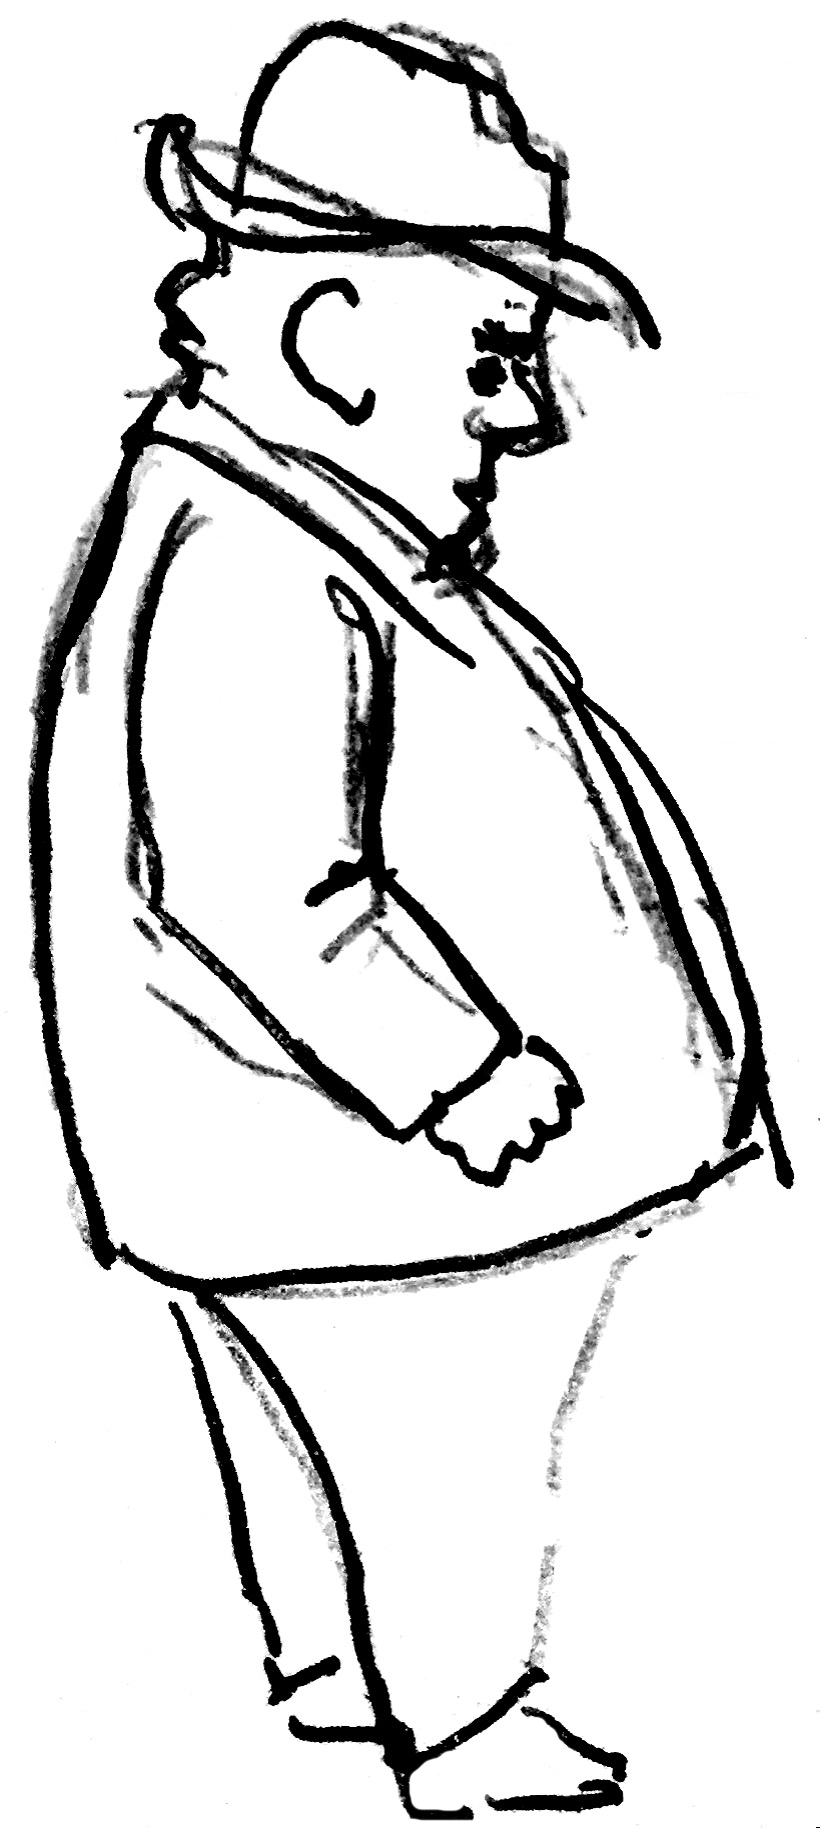
\includegraphics[width=0.6\textwidth]{Capelli_mangione}
    \caption[Capelli (Zucò 'd Capeli)]{}
    \vspace{-0.3cm}
\end{figure}

\newpage
\indent Teneva regalare copia e minute\footnote{Le prime stesure provvisorie delle lettere} delle lettere amorose che riceveva, la collezione dei ricciolini... e di altri peli ancor più fini...\\
\indent Dopo morto si trovò tutto questo materiale documentario della sua attività conquistatrice ed una cambiale, con la firma del povero \index[Personaggi]{Capelli (protocollista)}Capelli ed altra persona con accompagnato un biglietto così concepito:
\begin{center}
	\emph{Caro Capelli, vi mando la cambiale che avete firmato per me, che ho pagato, e che ora ha solo un valore di riconoscenza. Vi prego di distruggerla, perché se la trovano i vostri eredi diranno che vi siete mangiati anche quelli...}
\end{center}

 \begin{figure}[htb]
    \centering
    %\vspace{-0.7cm}
    \includegraphics[width=\textwidth]{mingò}
    \caption[Gruppo Montecatini di Alfonsine]{L'uomo con gli occhiali seduto al centro è \textbf{Domenico Soatti}, "Mingò 'd Galèna"\index[Personaggi]{Domenico Soatti `Mingò d'Galèna` (infermiere)}, mentre i due uomini in piedi sulla destra, partendo da sinistra sono: Stefano Mingazzi e \index[Personaggi]{Isani Nando}Nando Isani\label{fig:mingò}. L'uomo con il camice a sinistra è Domenico Stella\index[Personaggi]{Stella dott. Domenico}.}
    %\vspace{-0.3cm}
\end{figure}

\newpage
\subsection{Gioti}
Questo capitoletto è presente nell'indice, ma non fu mai scritto. Questo è ciò che ho trovato nel quaderno:\\
\begin{figure}[!htbp]
   \includegraphics[width=\textwidth]{"Gioti".jpg}
\end{figure}
\\Probabilmente Mingazzi voleva scrivevere qualche racconto su \index[Personaggi]{Marchiani Luigi `Gioti'}Marchiani Luigi (08/06/1872 - 29/04/1934). Alcuni vecchi del paese ancora lo ricordano, sempre a spasso con il suo asinello.
\newpage
Riporto la prima pagina del racconto su Gioti della mia cara amica \index[Personaggi]{Forlivesi Edda}Edda Forlivesi.\\

 \begin{figure}[htb]
    \centering
    \vspace{-0.3cm}
    \includegraphics[width=\textwidth]{Gioti2}
    \vspace{-0.3cm}
\end{figure}

\noindent \textit{Traduzione}: Gioti stava nella casa dei Zalambani, quella che hanno buttato giù; là c'era il circolo, e sotto al circolo di Vincenzo Monti, c'era Gioti, e lì in tutta quanta la casa vecchia, comandava Bosi di Lugo. È stato 42 anni lì e non ha mai pagato l'affitto un anno. Un bel giorno arriva Bosi di Lugo e gli dice: <<Ciò, Marchiani (lui si chiamava Marchiani) qui...>> (lui faceva il sarto e la mattina prendeva il somaro che lo chiamava `Girardengo', e poi andava a contadini. Tornava a casa la sera, come al solito, sempre ubriaco).\\
\indent E una mattina arriva Bosi, lui è lì che prende il somaro e gli fa:\\
\indent <<Ciò Marchiani, qui se non paghi l'affitto, sono costretto a mandarvi via da qui!>>\\
\indent <<Eccolo, finisco di mettere le redini al somaro e poi me ne vado subito!>>\\
\indent <<No, no, qui, o comprate oppure ve ne andate!>>\\
\indent <<Io pensavo di vendere>> gli rispose Gioti.\\




























%-------------------------------------------------------------------------------
%	CAPITOLO 42
%-------------------------------------------------------------------------------

\chapter{Il Capitano}
Anche questo capitolo è presente nell'indice ma purtroppo non è mai stato scritto. Tuttavia, nel raccoglitore di mio nonno ho trovato una lettera insieme ai manoscritti. Questa lettera è indirizzata a Stefano Mingazzi ed è firmata \emph{G. De Maria}. Giuseppe De Maria (cav.)\index[Personaggi]{De Maria Giuseppe} fu sindaco di Alfonsine nel 1902 e fu farmacista. Probabilmente Mingazzi chiese a Giuseppe De Maria qualche informazione sul \emph{Capitano Lucidi}, ovvero \index[Personaggi]{Lucidi Pietro (assessore)}Pietro Lucidi, che fu assessore delegato.  \\
Riporto fedelmente il contenuto della lettera:\\\\
\emph{
\rightline{Roma 28.10.1942}
Gentilissimo Stefano,\\
Subito dopo il ritorno di Nando e della Clara a Roma sono stato colto dell'influenza. Questa è la sola ragione per cui la mia risposta le giunge con tanto ritardo.\\
Io sarei stato ben lieto di poterle fornire notizie inedite sul Capitano Lucidi; ma da quello che m'ha raccontato la Clara, Lei, benché comparso sulla scena del mondo ben tardi, conosce di questa macchietta tutta la ridicola istoria.\\
In una zirudela stampata alla macchina verso il 1880 e attribuita al maestro \index[Personaggi]{Castellani Giulio (avvocato)}Castellani ecco com'era dipinto quest'imbecille:
\begin{verse}
	E Badoia e vó sté d'sora\\
	E e dis: "ostia, va in malora!"\\
	Lò beet cun e su amor\\
	a squicer a totti agli or\\
	Il sa tott che é su zarvell\\
	Uiè scap d'sotta e cappell
\end{verse}
Rovistando nel mio disordinato archivio ho trovato un brutto sonetto che riguarda il Capitano, che io composi, se non erro nel 1887. Esso mi fu ispirato da una scena violenta avvenuta sulla piazza di Alfonsine, provocata da rivalità in amor, fra il \index[Personaggi]{Capitano}Capitano e certo Cavour, calzolaio, conosciuto anche come figlio di \index[Personaggi]{Bigano (fabbro)}Bigano, il quale, Cavour, mi pare che morisse al manicomio.\\
Nel sonetto è il Capitano che parla:
\begin{verse}
	Con la zanetta di legnoso albano(1),\\
	Passeggiavo su e giù per la Viulina (2)\\
	Quando un tal mi gridò: "Vecchio marrano,\\
	Ho voglia di scherzar questa mattina..."\\
	\rule{1.5cm}{0.4pt}\\
	Tosto confabulai: Chi sei prusano?\\
	Non sai che il mondo al mio voler s'inchina?\\
	Io son, rispose, il tuo rival Bigano,\\
	Quel Bigano che vuole la tua rovina!\\
	\rule{1.5cm}{0.4pt}\\
	Sbigutito livai la mia zanetta,\\
	Ma quel sicario m'afferrò pel collo\\
	Gridando: Puttanier, voglio vendetta!\\
	\rule{1.5cm}{0.4pt}\\
	Che spavento Gaitano,(3) che tracollo!\\
	Per fortuna fui tolto dalla stretta...\\
	Fratel, metti il pisodio a prutocollo! (4)\\
\end{verse}
1) Albàno invece di ebano. Il Capitano narrava spesso che "Venezia era fabbricata sopra dei pitoni di albàno!"\\
2) La \index[Luoghi]{Violina (via)}Viulina: ora via Abele Faccani\\
3) \index[Personaggi]{Lucidi Gaetano}Gaetano Lucidi, protocollista del Comune era fratello del Capitano\\
4) All'epoca del fattaccio, il Capitano funzionava da Sindaco e riteneva che la storia si sarebbe interessata dé suoi casi. Pisodio invece di episodio. \\
\\
Il capitano nella sua miserabile giovinezza si era arruolato in una compagnia di commedianti di passaggio per Alfonsine. Perciò tornato vecchio al suo paese volle dare un saggio della sua abilità come attore e si unì ai filodrammatici recitando la parte di Guglielmo nei "Due Sergenti". Io recitai con lui nello stesso dramma. Ma più che degli errori di cui infarciva la sua parte (Es. "Una borsa piena di doro") era la sua recitazione che faceva sbellicare dalle risa. Ora di tale recitazione potrò darle un saggio se Lei mi onora di una sua visita. Verbalmente potrò meglio illustrarlo quello che ha serivo. Mi riverisca la sua signora e Lei gradisca l'espressione della mia affettuosa amicizia,\\
\rightline{Suo att.mo G. De Maria}
\\\\P.S. Nando e la Clara mandano a Lei e alla Signora Amalia, a mio mezzo, i loro cordiali e rispettosi saluti.
}\\

\noindent Riporto la facciata della lettera nella pagina seguente.\\
 \begin{figure}[htb]
    \centering
    %\vspace{-0.7cm}
    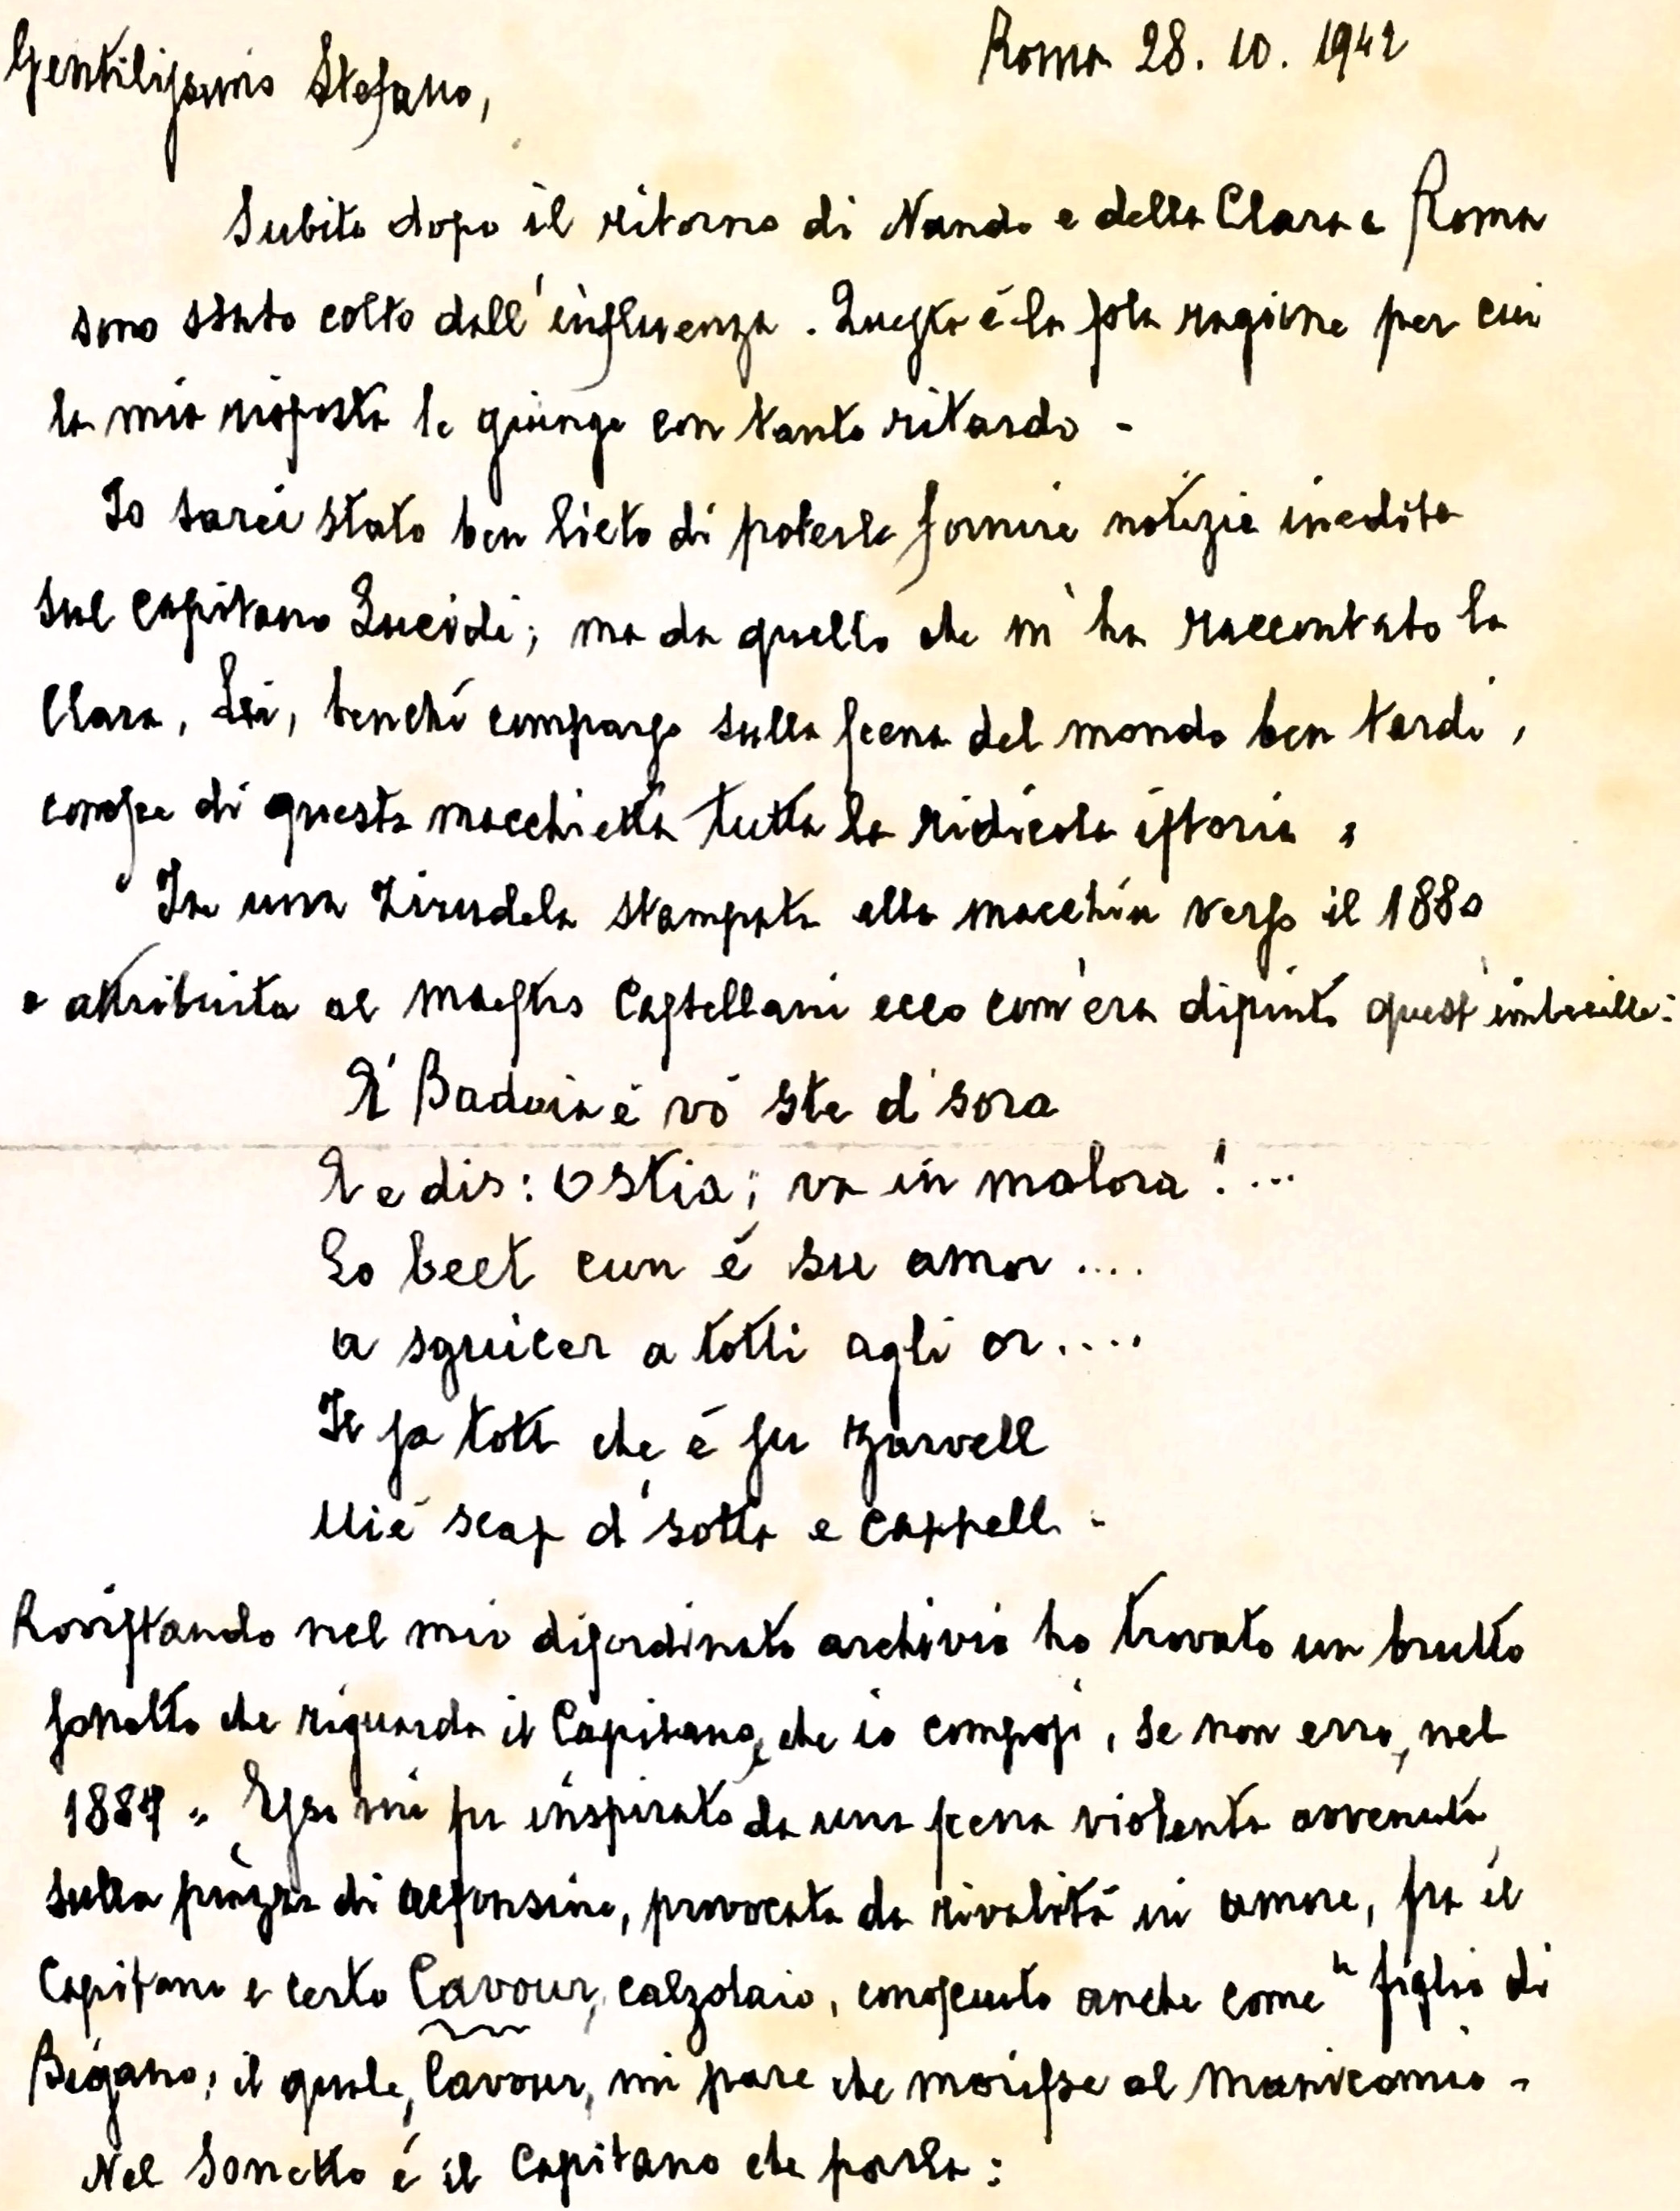
\includegraphics[width=\textwidth]{lettera}
    %\vspace{-0.3cm}
\end{figure}


%-------------------------------------------------------------------------------
%	CAPITOLO 43
%-------------------------------------------------------------------------------

\chapter{Capitoli mai scritti}
Nel retro dell'ultimo quaderno ho trovato alcuni appunti e titoli di capitoli  a matita che Mingazzi non è mai riuscito a scrivere. Vi riporto le annotazioni:\\
\\\emph{Ed ecco Alessandrino dei miei Natali\\
Coi suoi coniughi e le cubicazioni\\
Che per virtù di cappe e di piviali\\
Divenne anche Assessor dei matrimoni
\\\index[Personaggi]{Natali Alessandro (assessore)}
\rule{1.5cm}{0.4pt}\\
\\
Don \index[Personaggi]{Don Servidei Serafino}Servidei\footnote{Don Serafino Servidei fu il parroco presente durante la settimana rossa ad Alfonsine}
\\
\rule{1.5cm}{0.4pt}\\
\\
Il Santo
\\
\rule{1.5cm}{0.4pt}\\
\\
\index[Personaggi]{Fabbri Cesare}Fabbri Cesare (ricordi funebri (cavallo))}\\\\

\newpage

\noindent In allegato vi era anche questo appunto:\\

\noindent \emph{Casa posta sulla via\\
elta o basa che la sia\\
quand cla pies e su patron\\
cusavut te e mi cuion}\\
\begin{figure}[hbt]
\begin{center}
\vspace{-10pt}
   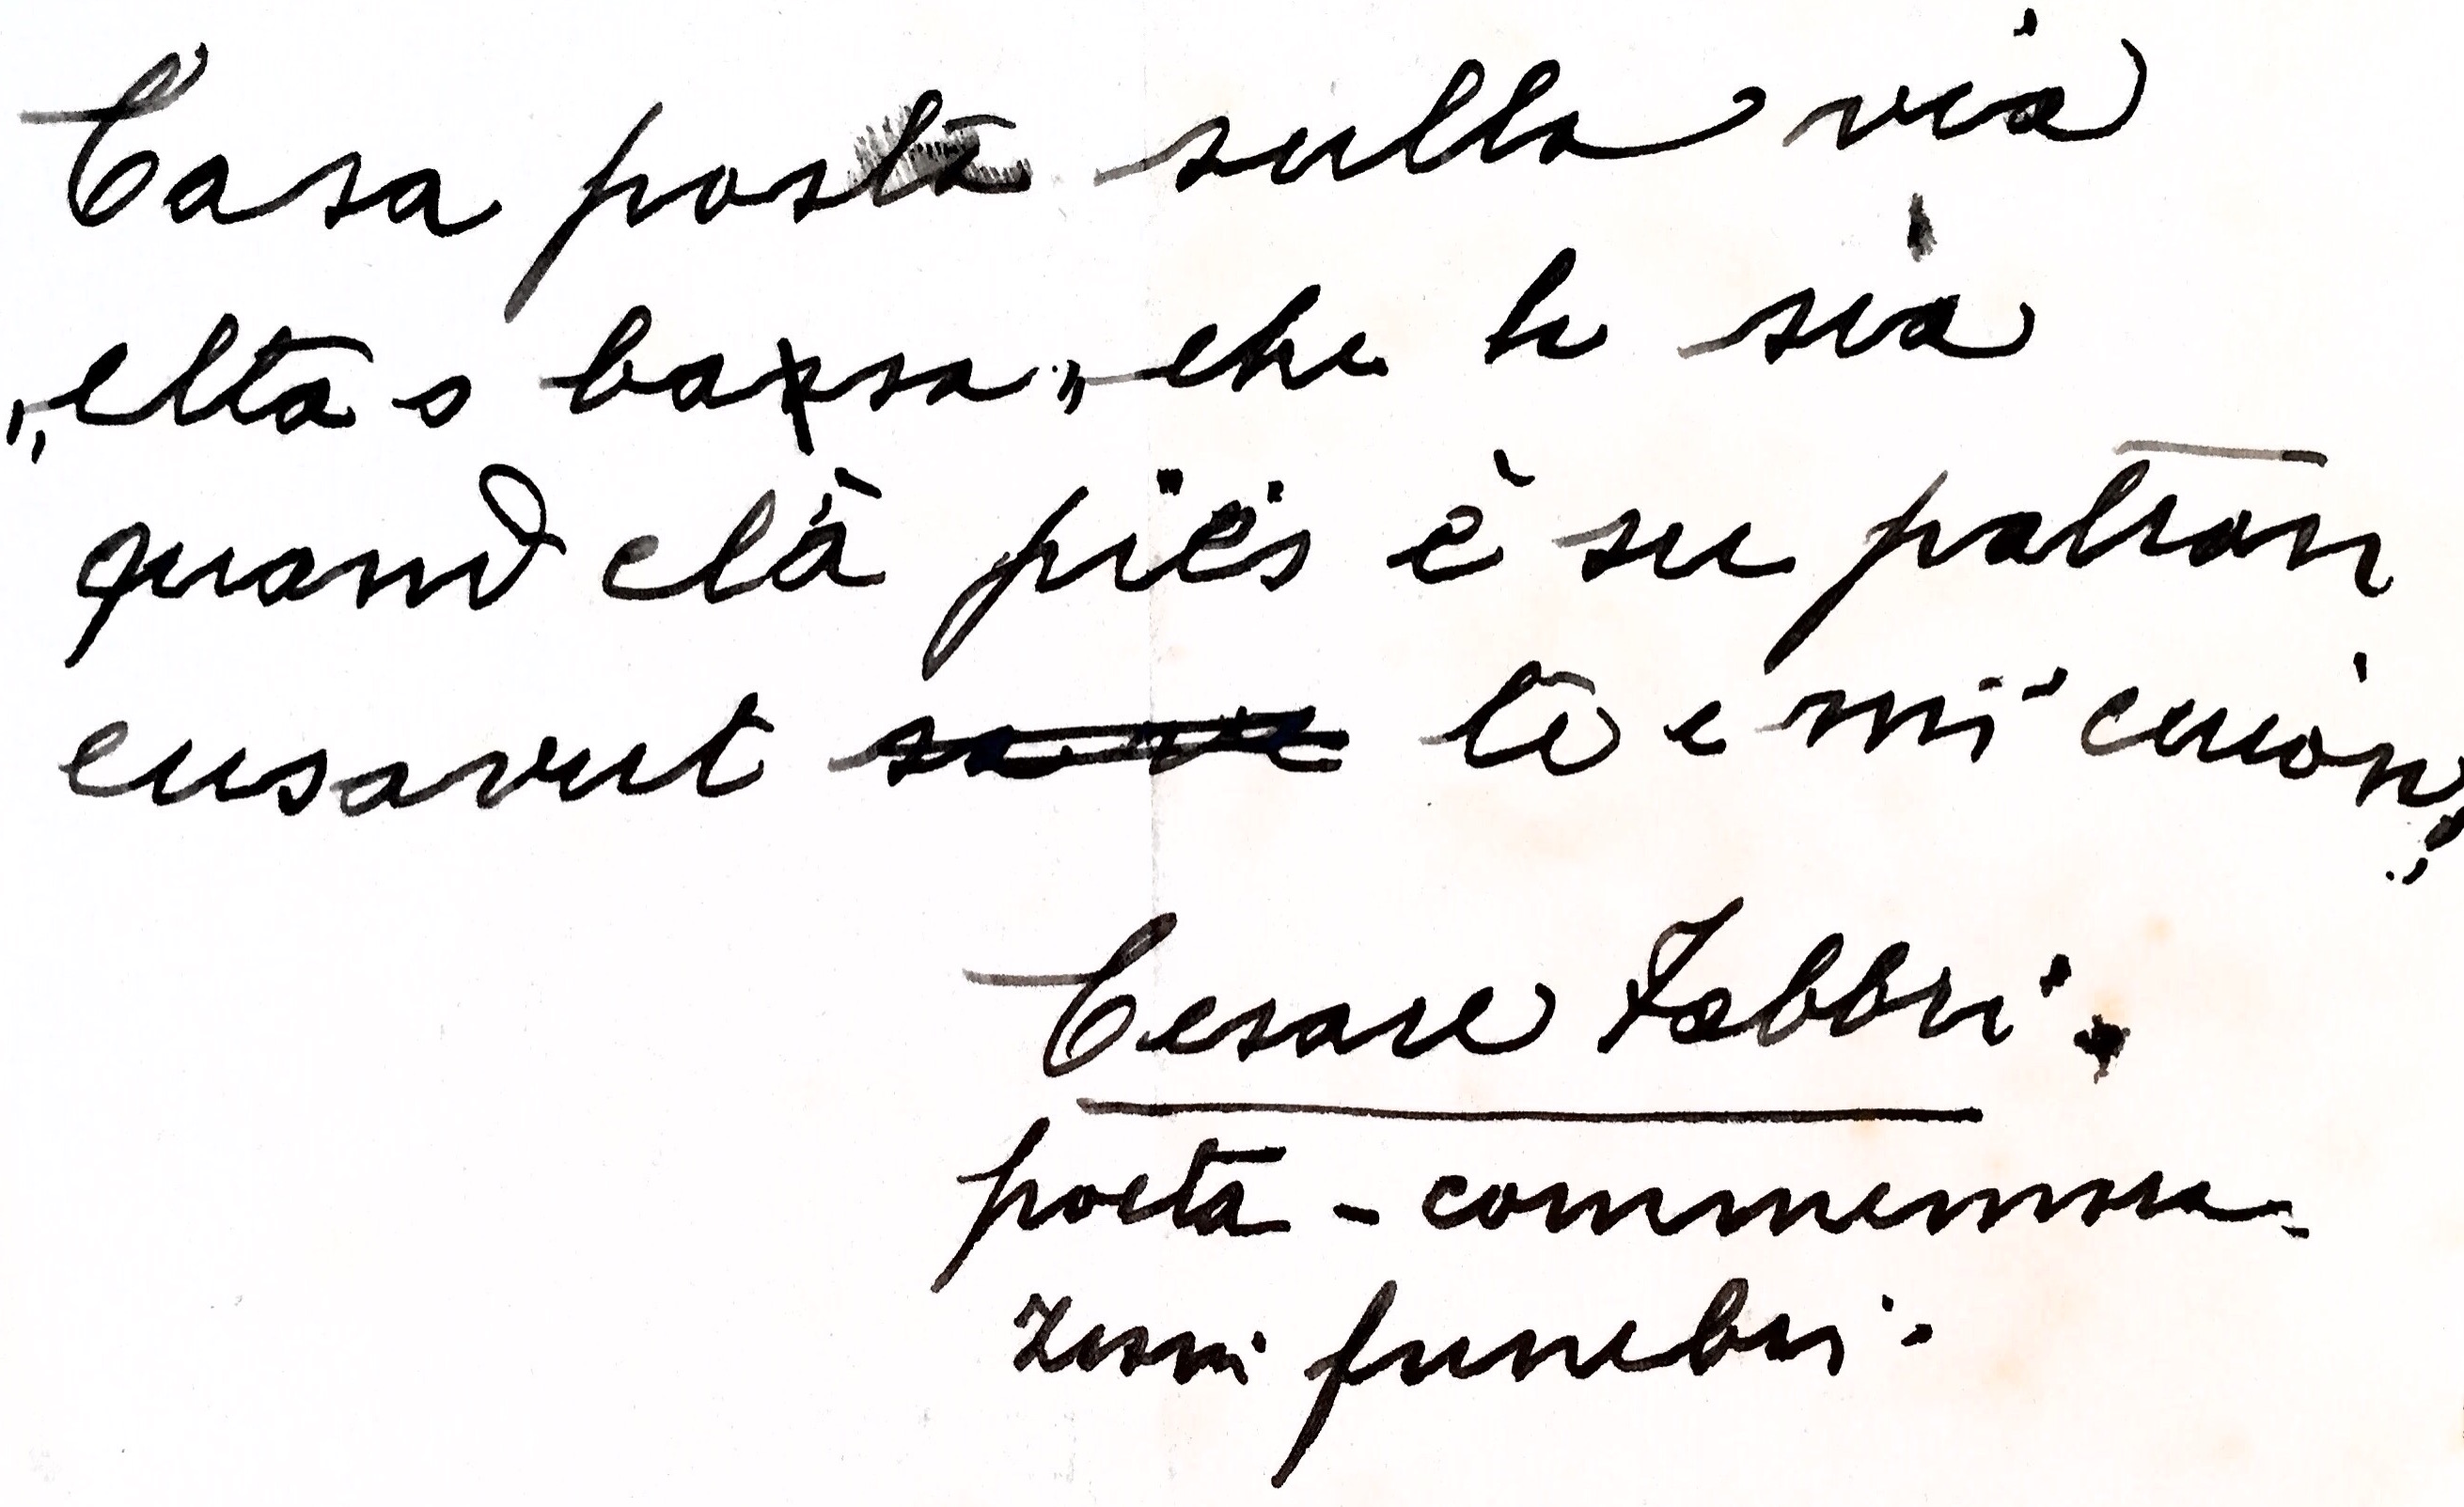
\includegraphics[width=\textwidth]{FabbriCesare}
  \end{center}
\end{figure}

\rule{1.5cm}{0.4pt}\\
\\
\emph{Don \index[Personaggi]{Don Battista}Battista (è proibito friggere nella padella, la signora E. M. rise: "io friggerò in una casseruola")}




%





%=============================================================================

%-----------------------------------------------------------------------------
%	INDEX: PERSONAGGI
%-----------------------------------------------------------------------------
\label{Personaggi}
\indexprologue{L'indice che segue, contiene tutti i nomi delle persone citate nel libro}
\printindex[Personaggi]

%-----------------------------------------------------------------------------
%	INDEX: LUOGHI
%-----------------------------------------------------------------------------
\label{Luoghi}
\indexprologue{Questo indice contiene tutti i luoghi, le vie, le chiese ed i palazzi contenuti nelle storielle.}
\printindex[Luoghi]

\newpage
%il codice seguente elimina gli spazi nella lista delle figure tra
% tra un capitolo e l'altro.

%-----------------------------------------------------------------------------
%	INDEX: Immagini
%-----------------------------------------------------------------------------
\label{Immagini}
\listoffigures


%=============================================================================

\end{document}